\documentclass[11pt,a4paper]{article}
\usepackage[utf8]{inputenc}
\usepackage[italian]{babel}
\usepackage{amsmath}
\usepackage{amsfonts}
\usepackage{amssymb}
\usepackage{array}
\usepackage{graphicx}
\usepackage{float}
\usepackage{multirow}
\usepackage{color,colortbl}
\usepackage{hyperref}
\hypersetup{colorlinks,urlcolor=blue,linkcolor=black}
\usepackage{fancyhdr}
\usepackage{tabularx}
\usepackage{csquotes}
\usepackage{enumitem}
\usepackage[left=2cm,right=2cm,top=2cm,bottom=3cm]{geometry}
\usepackage{longtable}
\usepackage{ltablex}
\usepackage{titlesec}
\usepackage{lastpage}
\setcounter{secnumdepth}{4}
\setcounter{tocdepth}{4}
\pagestyle{fancy}
\fancyhf{}
\lhead{
\includegraphics[scale=0.07]{images/logo.png}}

\definecolor{LightBlue}{rgb}{0,0,0.5}
\definecolor{Gray}{gray}{0.8}
\definecolor{LightGray}{gray}{0.9}

\renewcommand {\footrulewidth}{0.2mm}
\lfoot {Piano di Qualifica}
\rfoot{Pagina \thepage\ di \pageref{LastPage}}

\usepackage{lipsum}
\begin{document}
	\begin{titlepage}
  \centering
	\scshape
	
	\vspace*{2cm}
	
\includegraphics[scale=0.7]{images/logo.png}
	\rule{\linewidth}{0.2mm}\\[0.37cm]
	{\Huge Piano di progetto}\\
	\rule{\linewidth}{0.2mm}\\[1cm]
	{\LARGE\bfseries Progetto Colletta - Gruppo OttoBit}\\[1cm]
	
	
	
	\begin{tabular}{>{\columncolor{Gray}}r | >{\normalfont}l}
		\rowcolor{LightBlue}		
		\multicolumn{2}{c}{\color{white}{Informazioni sul documento}}\\
		Versione & 1.0.0 \\
		Redazione & Benedetto Cosentino\\
							& Enrico Marcato\\
 		Verifica & Giovanni Peron\\
 		Responsabile & Benedetto Cosentino\\
 		Uso & Esterno\\
 																 		& Prof. Tullio Vardanega\\
 																		& Prof. Riccardo Cardin\\
 		\multirow[t]{-3}{*}{Destinatari}	& MIVOQ s.r.l\\
 		\hline
	\end{tabular}
\end{titlepage}
	\newpage
	{\def\arraystretch{2}\tabcolsep=10pt
	
	\section*{\centering Registro delle modifiche}
	\begin{tabularx}{\textwidth}{ c | c | p{3.5cm} | c | X }
		\rowcolor{LightBlue}
		\color{white}\bfseries Versione & \color{white}\bfseries Data & \color{white}\bfseries Autore & \color{white}\bfseries Ruolo & \multicolumn{1}{c}{\color{white}\bfseries Descrizione}\\[0.25cm]
		3.0.2 & 2019-05-08 & Enrico Marcato \newline Eleonora Peagno & Verificatore & Modificate tabelle test di sistema \\ \hline
		3.0.1 & 2019-04-28 & Eleonora Peagno & Verificatore & Modificate tabelle dei test secondo indicazioni esito RQ \\ \hline
		3.0.0 & 2019-04-11 & Giovanni Bergo & Responsabile & Approvazione per il rilascio \\ \hline
		2.1.0 & 2019-04-11 & Gianmarco Pettenuzzo & Verificatore & Verifica del documento \\ \hline
		2.0.2 & 2019-04-10 & Eleonora Peagno & Verificatore & Inseriti grafici livelli ISO/IEC 15504 \\ \hline
		2.0.2 & 2019-04-09 & Eleonora Peagno & Verificatore & Inserite tabelle test di unità e loro tracciamento \\ \hline
		2.0.1 & 2019-03-18 & Eleonora Peagno & Verificatore & Correzione secondo indicazioni esito RP \\ \hline
		2.0.0 & 2019-03-06 & Gianmarco Pettenuzzo & Responsabile & Approvazione per il rilascio \\ \hline
		1.1.0 & 2019-03-06 & Benedetto Cosentino & Verificatore & Revisione finale del documento \\ \hline
		1.0.6 & 2019-03-05 & Eleonora Peagno & Verificatore & Aggiunte appendici "esito delle revisioni" e "copertura dei requisiti", aggiunta nota sulle metriche software. Correzioni e modifiche varie \\ \hline
		1.0.5 & 2019-03-04 & Giovanni Bergo \newline Eleonora Peagno & Verificatore & Aggiunti test di validazione \\ \hline
		1.0.4 & 2019-03-04 & Eleonora Peagno & Verificatore & Aggiunti test di integrazione e appendice sulle metriche \\ \hline
		1.0.3 & 2019-02-22 & Eleonora Peagno & Verificatore & Aggiunta tabella degli obiettivi \\ \hline
		1.0.2 & 2019-02-18 & Giovanni Bergo & Amministratore & Classificazione obbiettivi\\ \hline
		1.0.1 & 2019-02-15 & Eleonora Peagno & Verificatore & Eliminazione capitoli 2 e 3 v1.0.0, stesura nuovo capitolo 2, aggiunta sezione sul ciclo di Demming in appendice, revisione generale del documento, struttura e contenuti. \\ \hline
		1.0.0 & 2019-01-11 & Benedetto Cosentino & Responsabile & Approvazione documento\\ \hline
		0.2.0 & 2019-01-11 & Giovanni Bergo & Verificatore & Verifica documento\\ \hline
		0.1.3 & 2019-01-10 & Michele Bortone & Amministratore & Incremento \S\ 2.6\\ \hline
		0.1.2 & 2019-01-08 & Giovanni Peron & Amministratore & Incremento \S\ appendice A, stesura \S\  4.1.2\\ \hline
		0.1.1 & 2019-01-02 & Michele Bortone & Amministratore & Risoluzione errori\\ \hline
		0.1.0 & 2018-12-27 & Giovanni Bergo & Verificatore & Verifica documento\\ \hline
		0.0.8 & 2018-12-26 & Michele Bortone & Amministratore & Avanzamento \S\ 3\\ \hline
		0.0.6 & 2018-12-19 & Michele Bortone & Amministratore & Incremento \S\ 2.6\\ \hline
		0.0.5 & 2018-12-19 & Giovanni Peron & Amministratore & Avanzamento \S\  2.5, 2.6, tabelle \S\ 4.\\ \hline
		0.0.4 & 2018-12-18 & Giovanni Peron & Amministratore & Tabella sezione \S\ 4 e stesura \S\ 2.4, 2.5, 2.6.\\ \hline
		0.0.3 & 2018-12-16 & Michele Bortone & Amministratore & Aggiornamento struttura documento\\ \hline
	0.0.2 & 2018-12-13 & Michele Bortone & Amministratore & Stesura sezione\S\ 2.2  e \S\ appendice B\\ \hline
		0.0.1 & 2018-12-13 & Giovanni Peron & Amministratore & Stesura sezione\S\ 2.1 e \S\ appendice A \\ \hline
		0.0.0 & 2018-12-06 & Giovanni Peron & Amministratore & Creazione documento e \newline sezione introduzione \\ \hline
	\end{tabularx}
	\newpage
	
	\tableofcontents
	\newpage
	\listoffigures
	\listoftables
	
	\newpage
	\section{Introduzione}
\subsection{Scopo del documento}
Lo scopo del seguente documento è quello di garantire la qualità* del prodotto software e di conseguenza dei processi* impiegati per la sua realizzazione. Questo documento sarà composto in maniera incrementale, verrà modificato e migliorato durante l'arco temporale del progetto*, in modo coerente al suo ciclo di vita. Nelle prossime pagine verranno quindi illustrate le strategie di verifica* e di validazione da utilizzare per tutto lo svolgimento del progetto. Queste tecniche serviranno ad assicurare che le attività vengano eseguite correttamente, individuando e correggendo tempestivamente eventuali errori.
\subsection{Scopo del prodotto}
Il prodotto ha lo scopo di realizzare una piattaforma collaborativa di raccolta dati.  La piattaforma consentirà ad degli allievi di svolere esercizi di analisi grammaticale proposti da i loro insegnanti.
Lo scopo finale della piattaforma è raccogliere dati relativi agli esercizi predisposti e al loro svolgimento, con il fine di utilizzare tali informazioni per insegnare l'analisi grammaticale ad un elaboratore; tramite tecniche di apprendimento automatico.\\
Le tipologie di utenti che usufruiranno di questo prodotto saranno:
\begin{itemize}
	\item insegnanti: prepareranno in modo semplice e rapido degli esercizi da somministrare ai propri allievi;
	\item allievi: eseguiranno gli esercizi ottenendo una valutazione immediata;
	\item sviluppatori: potranno accedere ai dati raccolti mediante la piattaforma per automatizzare il servizio.
\end{itemize}
\subsection{Note esplicative}
Tutti i termini marcati con un * ad apice presenti nel seguente documento trovano una definizione all'interno del \textit{Glossario}.\\
I nomi dei documenti interni/esterni prodotti dal gruppo OttoBit saranno scritti in corsivo.
\subsection{Riferimenti}
\subsubsection{Normativi}
\begin{itemize}
\item \textit{Norme di progetto}
\item \textit{Analisi dei requisiti}
\item Capitolato d'appalto Colletta: piattaforma raccolta dati di analisi di testo\footnote{\url{https://www.math.unipd.it/~tullio/IS-1/2018/Progetto/C2.pdf}}
\end{itemize}
\subsubsection{Informativi}
\begin{itemize}
	\item K. EL EMAM, A. BIRK, \textit{Validating the ISO/IEC 15504 measures of software development process capability}, in \enquote{The Journal of Systems and Software}, 51 (2000), pp. 119-149\footnote{\url{https://www.uio.no/studier/emner/matnat/ifi/INF5181/h11/undervisningsmateriale/reading-materials/Lecture-11/SPICE/elemam-jss2000.pdf}}
	\item ISO/IEC 15504:2006\footnote{\url{http://artemisa.unicauca.edu.co/~cardila/CS\_10c\_ISO\_15504-5\_\_2006.PDF}}
	\item ISO/IEC 9126\footnote{\url{https://en.wikipedia.org/wiki/ISO/IEC_9126}}
\end{itemize} 
	
	\newpage
	\section{Visione generale delle strategie di verifica}
\subsection{Obiettivi di qualità}
	Per garantire la qualità del prodotto e dei processi utilizzati per realizzarlo il team Ottobit si è proposto di fissare degli obiettivi da perseguire per tutta la durata del progetto.
	\subsubsection{Qualità dei processi}
	Per il conseguimento degli obiettivi riguardanti la qualità dei processi è stato deciso di adottare lo standard ISO/IEC 15504 anche detta SPICE* acronimo di Software Process Improvement and Capability Determination. Questo standard viene utilizzato per eseguire una valutazione concreta della qualità dei processi, inoltre permette la misurazione della capability dei processi. All'appendice A è presente una descrizione delle caratteristiche dello standard.
	\subsubsection{Qualità del prodotto}
		Per quanto riguarda la qualità del prodotto si è scelto, in comune accordo, di seguire una serie di normative facenti parte dello standard ISO/IEC 9126, che definisce un modello dei requisiti qualitativi del Prodotto. Un completo approfondimento sullo standard ISO/IEC 9126 si trova in appendice B.
\subsection{Organizzazione}
Per fare in modo che la qualità del prodotto finale rimanga entro i livelli prestabiliti, è necessario che ogni processo del progetto sia verificato prima di passare al successivo, al fine di intercettare eventuali errori ed evitarne la loro propagazione. Per essere certi di attuare la verifica nel modo corretto, i membri del gruppo dovranno attenersi ai principi definiti dagli standard scelti. In caso di perplessità potranno essere consultate le appendici di questo documento, dove vengono illustrati gli standard da rispettare per perseguire la qualità dei processi e del prodotto.

\subsection{Pianificazione strategica}
La strategia generale adottata è quella di automatizzare il più possibile le operazioni di verifica grazie all'utilizzo di strumenti volti allo scopo. L'obiettivo è avere un riscontro affidabile e misurabile che permetta di assicurare il grado di qualità stabilito precedentemente.  L'aspettativa è la riduzione del lavoro manuale permettendo così un'attività di verifica più semplice ed efficace.

\subsection{Responsabilità}
Il verificatore ha il compito accertare che ogni modifica al materiale che costituisce il prodotto (codice, documentazione), effettuate dalle altre figure, venga svolta nella maniera corretta e nel rispetto delle regole definite in questo documento. Il Responsabile di progetto ha il compito di coordinare tutte le attività di verifica e di fare da garante della corretta esecuzione di tali, al fine di mantenere la qualità del materiale prodotto durante il suo ciclo di vita. Una descrizione più approfondita dei ruoli di progetto è inclusa nel documento  \textit{PianoDiProgetto\_v1.0.0}.

\subsection{Risorse}
Per svolgere queste operazioni il verificatore usufruirà di alcune risorse. Principalmente queste si dividono in due tipologie, le risorse necessarie sono quelle indispensabili per compiere il lavoro di verifica, quelle disponibili sono risorse alle quali il verificatore può attingere per eseguire il suo compito in modo efficacie ed efficiente.

\subsubsection{Necessarie}
I risultati del lavoro del gruppo devono essere disponibili a chiunque si occupi della verifica. Dunque i documenti o i files prodotti devono essere accessibili dal verificatore. Quest'ultimo dovrà disporre anche di un sistema per comunicare il risultato della verifica e i conseguenti problemi e cambiamenti da apportare, in modo che chi dovere posa porre rimedio alle mancanze nel più breve tempo possibile.

\subsubsection{Disponibili}
Il verificatore avrà a disposizione diversi strumenti per ottimizzare il processo di verifica e di valutazione. I documenti saranno fruibili dalla repository condivisa tra i membri del gruppo attraverso la piattaforma GitLab*. I verificatori utilizzeranno un calcolatore di indice di Gulpease e gli strumenti forniti dall'editor Latex per notare meglio errori ortografici. Per notificare l'esito della verifica il verificatore potrà avvalersi di GitLab, del gruppo su Slack oltre alla tabella di resoconto nella sezione 4 del \textit{PianoDiQualifica\_v1.0.0}.

\subsection{Tecniche di verifica}
Per eseguire la verifica e la validazione potranno essere utilizzate tecniche di analisi statica o dinamica. Le prime sono le tecniche che si concentrano sullo studio della documentazione e del codice per accertarsi della presenza delle proprietà desiderate, l'assenza di difetti, e della conformità alle regole. A differenza di quelle statiche le tecniche di analisi dinamica richiedono l'esecuzione del codice e la verifica viene effettuata tramite prove del prodotto.\\
L'applicazione pratica delle tecniche di seguito presentate viene trattata nelle \textit{NormeDiProgetto\_v1.0.0}, affinché i membri del gruppo possano sempre avere un riferimento comune sulla verifica della qualità.
\subsubsection{Analisi statica}
Per la verifica della documentazione dovranno essere analizzate la correttezza grammaticale e ortografica, la correttezza degli argomenti trattati, la struttura del documento. Verranno utilizzati a questo scopo i correttori ortografici presenti negli editor Latex. Inoltre verrà calcolato l'indice di Gulpease per ogni documento redatto, grazie al quale sarà possibile valutare la complessità sintattica e la leggibilità del documento.\\
Per verificare il codice dell'applicazione che verrà creata sarà necessario analizzare diversi aspetti:
\begin{itemize}
\item Analisi del flusso di controllo: è necessaria per assicurarsi che il codice esegua nella sequenza desiderata e che esso sia ben strutturato. Non devono esistere parti di codice irraggiungibili o interminabili.
\item Analisi del flusso dei dati: controlla che non vengano utilizzate variabili senza che queste non siano state prima inizializzate. Non devono esistere variabili inutilizzate. 
\item Analisi del flusso di informazione: consiste nell'identificare le dipendenze tra informazioni passate in input e quelle prodotte in output dall’esecuzione di una unità di codice. Per assicurarsi che vengano rispettate le dipendenze previste e che non ci siano side effects indesiderati.
\end{itemize}
Questi tre aspetti potranno essere valutati grazie ad opportune misurazioni sulla complessità ciclomatica, numero di classi e coesione tra esse, complessità di flusso di informazioni.
\newpage
\subsubsection{Analisi dinamica}
L’analisi dinamica è il processo di valutazione di un sistema software o di un suo componente basato sull’osservazione del suo comportamento in esecuzione.
I componenti software che insieme formano il prodotto dovranno essere verificati attraverso diversi tipi di test, con lo scopo di garantire il corretto funzionamento dell'intero prodotto software.
I test effettuati devono essere:
\begin{itemize}
\item misurabili e oggettivi;
\item ripetibili nel tempo, anche dopo una modifica al sistema;
\item eseguiti in una quantità sufficiente da provare la qualità del prodotto.
\end{itemize} 
	\newpage
	\appendix
\section{Specifica dei test}
\subsection{Test di validazione}
Questo tipo di test verrà utilizzato durante l'attività di collaudo del prodotto finale così da accertare che esso soddisfi le richieste del committente. Per ogni test viene specificato il proprio codice univoco, il codice identificativo del requisito ad esso associato, la descrizione e lo stato di implementazione attuale. 
{\renewcommand{\arraystretch}{2}%
	\begin{longtable}{|>{\centering\arraybackslash}m{1.6cm}|>{\centering\arraybackslash}m{6.41cm}|>{\centering\arraybackslash}m{3.1cm}|}		
		\rowcolor{LightBlue}
		\textbf{\textcolor{white}{Test}}
		& \multicolumn{1}{|c|}{\textbf{\textcolor{white}{ Descrizione}}}
		& \textbf{\textcolor{white}{Esito}}\\
		
		\caption{Test di validazione}
\end{longtable}}

\subsection{Test di sistema}
Di seguito riportiamo una tabella contenente i test di sistema che intendiamo implementare per la verifica dei requisiti funzionali specificati nell'\emph{Analisi dei requisiti}. Per ogni test viene specificato il proprio codice univoco, il codice identificativo del requisito ad esso associato, la descrizione e lo stato di implementazione attuale.
{\renewcommand{\arraystretch}{2}%
	\begin{longtable}{|>{\centering\arraybackslash}m{1.6cm}|>{\centering\arraybackslash}m{1.7cm}|m{6.41cm}|>{\centering\arraybackslash}m{3.1cm}|}		
		\rowcolor{LightBlue}
		\textbf{\textcolor{white}{Codice\newline test}}
		& \textbf{\textcolor{white}{Codice\newline requisito}}
		& \multicolumn{1}{|c|}{\textbf{\textcolor{white}{ Descrizione}}}
		& \textbf{\textcolor{white}{Stato}}\\
		
		\hline
		\rowcolor{LightGray}
		TS-RO1
		& ROF1 
		& Verifica che l'utente riesca a registrarsi alla piattaforma creando un account personale. 
		& non implementato\\ \hline
		\rowcolor{white}
		TS-RO2
		& ROF2 
		& Verifica che l'utente possa eseguire l'accesso alla piattaforma utilizzando le sue credenziali.
		& non implementato\\ \hline
		\rowcolor{LightGray}
		TS-RD1
		& RDF1 
		& Verifica che l'utente possa modificare i dati del proprio profilo personale.
		& non implementato\\ \hline
		\rowcolor{white}
		TS-RD2
		& RDF2 
		& Verifica che l'amministratore possa verificare le credenziali di un utente che richiede la registrazione come insegnante. 
		& non implementato\\ \hline
		\rowcolor{LightGray}
		TS-RD3
		& RDF3 
		& Verifica che l'utente venga avvisato in caso di errore nell'inserimento dei dati richiesti.
		& non implementato\\ \hline
		\rowcolor{white}
		TS-RO3		
		& ROF3 
		& Verifica che l'insegnante e l'allievo possano ricercare degli esercizi sulla piattaforma.
		& non implementato\\ \hline
		\rowcolor{LightGray}
		TS-RP1		
		& RPF1 
		& Verifica che durante la ricerca, l'utente abbia la possibilità di impostare dei filtri per raffinarla. 		
		& non implementato\\ \hline
		\rowcolor{white}
		TS-RD4		
		& RDF4 
		& Verifica che dopo una ricerca, l'utente venga avvisato con un messaggio nel caso in cui il sistema non abbia trovato nessun risultato corrispondente ai criteri selezionati.
		& non implementato\\ \hline
		\rowcolor{LightGray}
		TS-RP2		
		& RPF2 
		& Verifica che l'amministratore possa eliminare un utente iscritto alla piattaforma.
		& non implementato\\ \hline
		\rowcolor{white}
		TS-RP3		
		& RPF3 
		& Verifica che l'insegnante possa modificare una soluzione di un esercizio da lui fornita
		& non implementato\\ \hline
		\rowcolor{LightGray}
		TS-RD5		
		& RDF5 
		& Verifica che l'insegnante, accedendo alla sua area del profilo, possa visualizzare la lista degli esercizi da lui creati. 
		& non implementato\\ \hline
		\rowcolor{white}
		TS-RP4		
		& RPF4 
		& Verifica che l'insegnante possa eliminare una soluzione di un esercizio da lui fornita. 
		& non implementato\\ \hline
		\rowcolor{LightGray}
		TS-RP5		
		& RPF5 
		& Verifica che l'insegnante possa indicare gli argomenti trattati nell'esercizio in fase di creazione.
		& non implementato\\ \hline
		\rowcolor{white}
		TS-RO4		
		& ROF4 
		& Verifica che l'allievo possa inserire una frase da svolgere o selezionare un esercizio da quelli disponibili sul sistema.
		& non implementato\\ \hline
		\rowcolor{LightGray}
		TS-RO5		
		& ROF5 
		& Verifica che l'allievo possa compilare i campi relativi alle parole della frase al fine di completare l'esercizio selezionato.
		& non implementato\\ \hline
		\rowcolor{white}
		TS-RD6		
		& RDF6 
		& Verifica che lo sviluppatore possa ricercare le annotazioni di una particolare frase.
		& non implementato\\ \hline
		\rowcolor{LightGray}
		TS-RP6		
		& RPF6 
		& Verifica che lo sviluppatore possa ordinare la lista dei risultati ottenuti dalla ricerca tramite determinati parametri. 
		& non implementato\\ \hline
		\rowcolor{white}
		TS-RP7		
		& RPF7 
		& Verifica che l'amministratore possa eliminare uno qualsiasi degli esercizi inseriti nel sistema.
		& non implementato\\ \hline
		\rowcolor{LightGray}
		TS-RO6		
		& ROF6 
		& Verifica che l'insegnante possa inserire un esercizio nel sistema, indicando una soluzione per esso. 
		& non implementato\\ \hline
		\rowcolor{white}
		TS-RO7		
		& ROF7 
		& Verifica che l'insegnante possa inserire la soluzione dell'esercizio che sta creando; può renderla pubblica o privata. 
		& non implementato\\ \hline
		\rowcolor{LightGray}
		TS-RO8		
		& ROF8 
		& Verifica che l'allievo possa svolgere un esercizio da lui indicato e visualizzarne la relativa valutazione. 
		& non implementato\\ \hline
		\rowcolor{white}
		TS-RD7		
		& RDF7 
		& Verifica che l'allievo, accedendo al proprio profilo, possa visualizzare dei dati relativi ai propri progressi. 
		& non implementato\\ \hline
		\rowcolor{LightGray}
		TS-RD8		
		& RDF8 
		& Verifica che lo sviluppatore possa filtrare i dati trovati durante la ricerca ottenendo una lista di esercizi. 
		& non implementato\\ \hline
		\rowcolor{white}
		TS-RD9
		& RDF9 
		& Verifica che lo sviluppatore possa impostare un filtro temporale per la ricerca degli esercizi.
		& non implementato\\ \hline
		\rowcolor{LightGray}
		TS-RD10		
		& RDF10 
		& Verifica che lo sviluppatore possa includere o escludere dalla ricerca uno o più utenti. 
		& non implementato\\ \hline 
		\rowcolor{white}
		TS-RP8		
		& RPF8 
		& Verifica che lo sviluppatore possa visualizzare i dati relativi ad una particolare annotazione. 		
		& non implementato\\ \hline
		\rowcolor{LightGray}
		TS-RP9		
		& RPF9 
		& Verifica che lo sviluppatore possa visualizzare lo storico delle annotazioni. 
		&  non implementato\\ \hline
		\rowcolor{white}
		TS-RO9
		& ROF9 
		& Verifica che lo sviluppatore deve poter scaricare un file contenente i dati relativi agli esercizi ottenuti con la ricerca.
		& non implementato\\ \hline
		\rowcolor{LightGray}
		TS-RP10		
		& RPF10 
		& Verifica che lo sviluppatore può visualizzare le informazioni relative ad uno dei modelli disponibili. 
		& non implementato\\ \hline
		\rowcolor{white}
		TS-RP11		
		& RPF11 
		& Verifica che lo sviluppatore deve poter scaricare le informazioni riguardanti un modello. 
		& non implementato\\ \hline
		\rowcolor{LightGray}
		TS-RP12		
		& RPF12 
		& Verifica che lo sviluppatore deve poter creare un modello tramite la piattaforma. 
		& non implementato\\ \hline	
		
		\rowcolor{white}
		TS-RO10	
		& ROF10 
		& Verifica che l'insegnante possa creare una nuova classe. 
		& non implementato\\ \hline
		\rowcolor{LightGray}
		TS-RO11	
		& ROF11 
		& Verifica che l'insegnante possa eliminare una classe dal sistema. 
		& non implementato\\ \hline
		\rowcolor{white}
		TS-RO12
		& ROF12 
		& Verifica che l'insegnante possa aggiungere degli alunni ad una classe. 
		& non implementato\\ \hline
		\rowcolor{LightGray}
		TS-RO13
		& ROF13 
		& Verifica che l'insegnante possa aggiungere degli esercizi a quelli assegnati ad una classe. 
		& non implementato\\ \hline
		\rowcolor{white}
		TS-RP13
		& RPF13 
		& Verifica che l'insegnante possa visualizzare i progressi degli alunni di una propria classe.
		& non implementato\\ \hline
		\rowcolor{LightGray}
		TS-RO14
		& ROF14 
		& Verifica che l'insegnante possa eliminare un alunno dalla lista di quelli iscritti ad una delle proprie classi. 
		& non implementato\\ \hline
		\rowcolor{white}
		TS-RO15	
		& ROF15 
		& Verifica che l'insegnante possa visualizzare la lista degli alunni iscritti ad una delle sue classi. 
		& non implementato\\ \hline
		\rowcolor{LightGray}
		TS-RO16
		& ROF16 
		& Verifica che l'utente possa visualizzare la lista delle proprie classi. 
		& non implementato\\ \hline
		\rowcolor{white}
		TS-RD11	
		& RDF11 
		& Verifica che l'utente possa confermare le operazioni.
		& non implementato\\ \hline
		
		\caption{Test di sistema}
\end{longtable}}

\subsection{Test di integrazione}
Questa tipologia di test serve per verificare che le varie componenti del sistema interagiscono tra loro nella maniera attesa. La strategia per definire i seguenti test è stata fatta partendo dalle singole componenti per poi realizzare le varie funzionalità in ordine di importanza. Per ogni test viene specificato il suo codice univoco, la descrizione e lo stato di implementazione attuale. APPROFONDIRE

{\renewcommand{\arraystretch}{2}%
	\begin{longtable}{|>{\centering\arraybackslash}m{1.6cm}|>{\centering\arraybackslash}m{6.41cm}|>{\centering\arraybackslash}m{3.1cm}|}		
		\rowcolor{LightBlue}
		\textbf{\textcolor{white}{Test}}
		& \multicolumn{1}{|c|}{\textbf{\textcolor{white}{ Descrizione}}}
		& \textbf{\textcolor{white}{Esito}}\\
		
		\hline
		TI1
		& Test d’integrazione finale tra l’applicazione Front-end e l’applicazione Back-end.
		& Non implementato
		\\ \hline
		
		
		\caption{Test di integrazione}
\end{longtable}}


\section{Resoconto attività di verifica}
\subsection{Prodotto}
\subsubsection{Documentazione}
Nella tabella seguente vengono riportati i risultati delle verifiche eseguite sui documenti. Il resoconto contiene le verifiche sia dei documenti esterni, cioè utili al committente, sia interni, utili invece al team Ottobit.\\
{\renewcommand{\arraystretch}{1.5}%
	\begin{longtable}{>{\centering\arraybackslash}m{3cm} >{\centering\arraybackslash}m{4cm} >{\centering\arraybackslash}m{5cm} >{\centering\arraybackslash}m{2cm}}
		\rowcolor{LightBlue}
		\textbf{\textcolor{white}{Documento}}
		& \textbf{\textcolor{white}{Indice Gulpease}}
		& \textbf{\textcolor{white}{Esito}}\\
		\textit{Studio di fattibilità v1.0.0} & 60 & Accettato\\
		\hline
		\rowcolor{LightGray}
		\textit{Analisi dei requisiti v1.0.0} & 82 & Accettato\\
		\hline
		\textit{Norme di progetto v1.0.0} & 67 & Accettato\\
		\hline
		\rowcolor{LightGray}
		\textit{Piano di qualifica v1.0.0} & 72 & Accettato\\
		\hline
		\textit{Piano di progetto v1.0.0} & 64 & Accettato\\
		\hline
		\caption{Resoconto attività di verifica}
	\end{longtable}
}

\subsubsection{Software}
TODO



\newpage
\subsection{Processi}
\subsubsection{Valori ISO/IEC 15504 - MPC1}

\paragraph{Revisione dei Requisiti}\noindent \\
Di seguito riportiamo le misurazioni dei processi più significativi sviluppati durante il periodo di Revisione dei Requisiti. Tali valori sono stati raccolti secondo la metrica MPC1 che fa riferimento alle linee guida dettate dallo standard ISO/IEC 15504
\subparagraph{Studio di fattibilità}
\noindent
\begin{figure}[H]
	\centering
	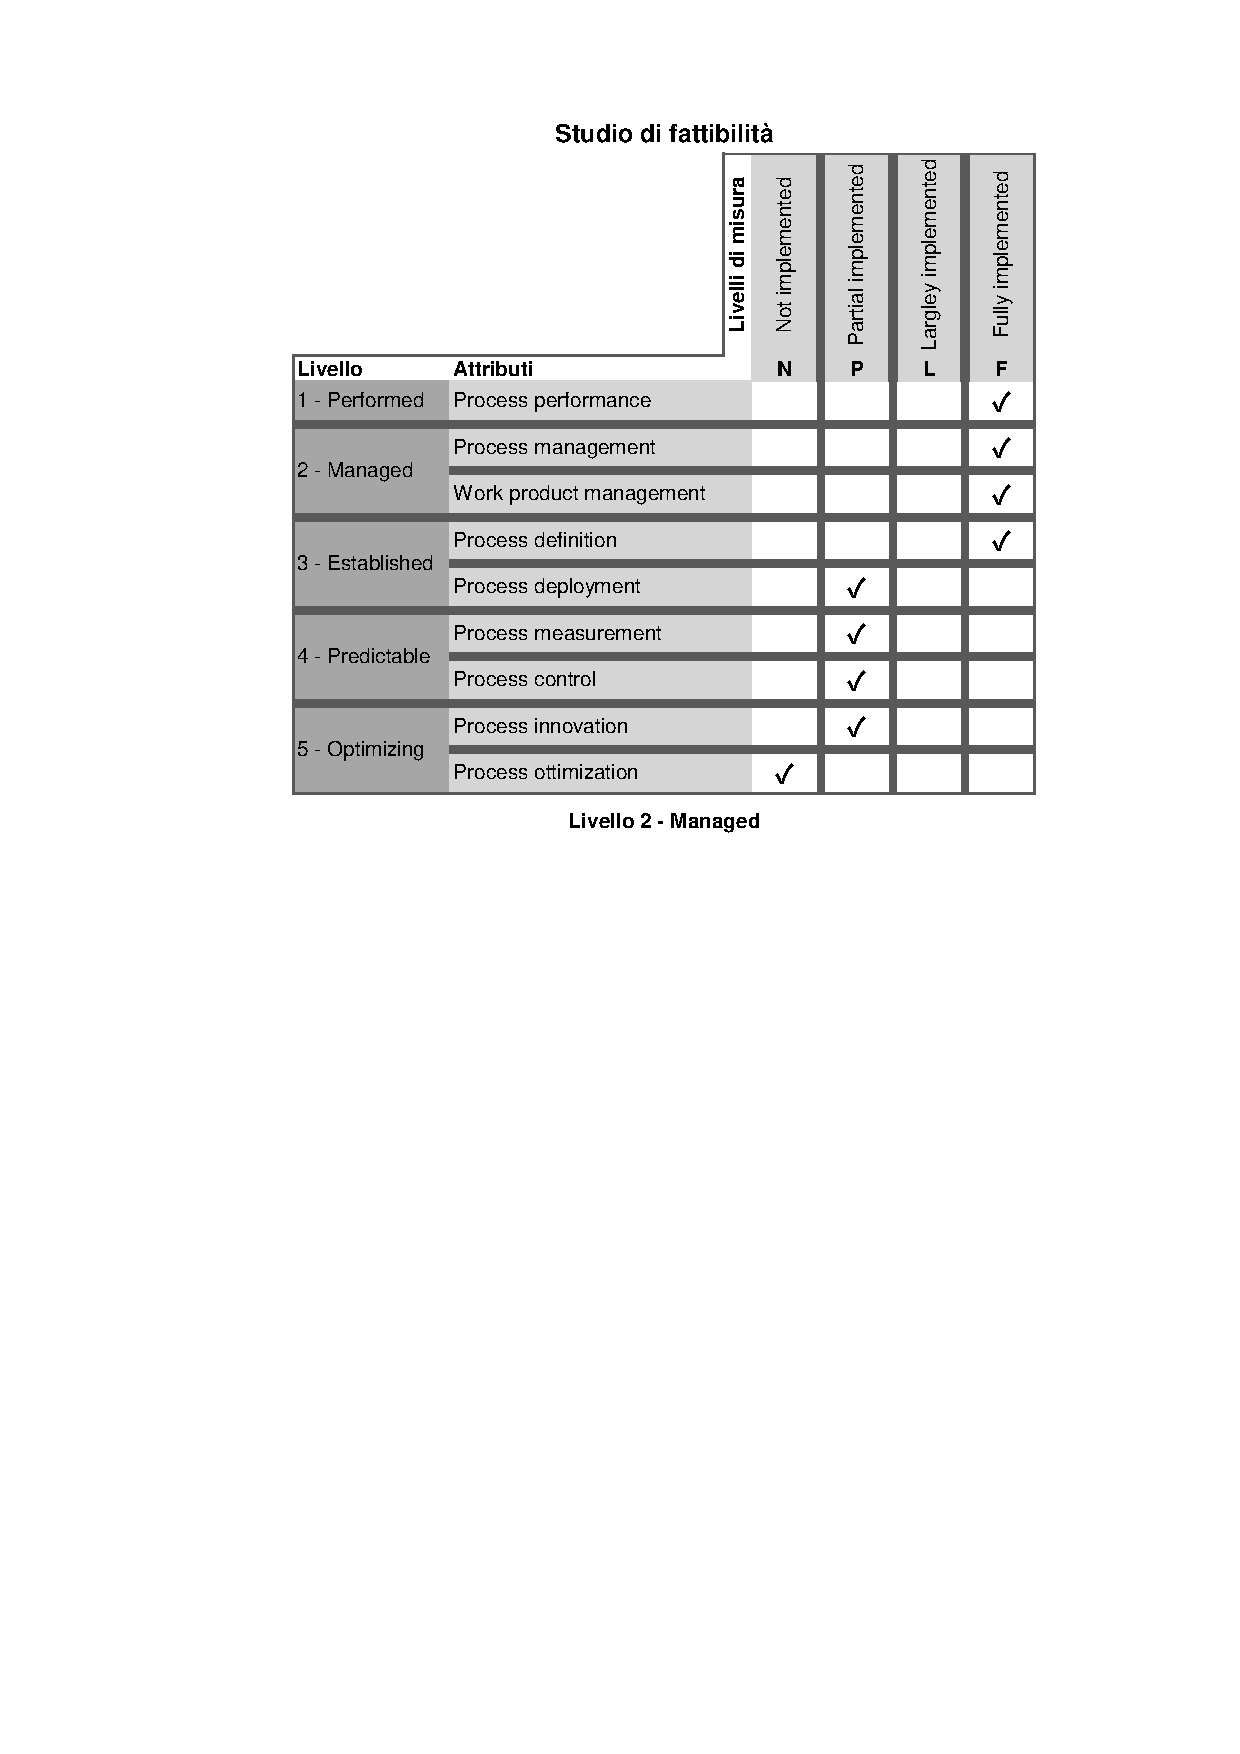
\includegraphics[scale=1]{images/resoconto/RR/studiodifattibilita-RR.pdf}
	\caption{Valori ISO/IEC 15504 Studio di fattibilità}	
\end{figure}
\newpage
\subparagraph{Norme di progetto}
\noindent
\begin{figure}[H]
	\centering
	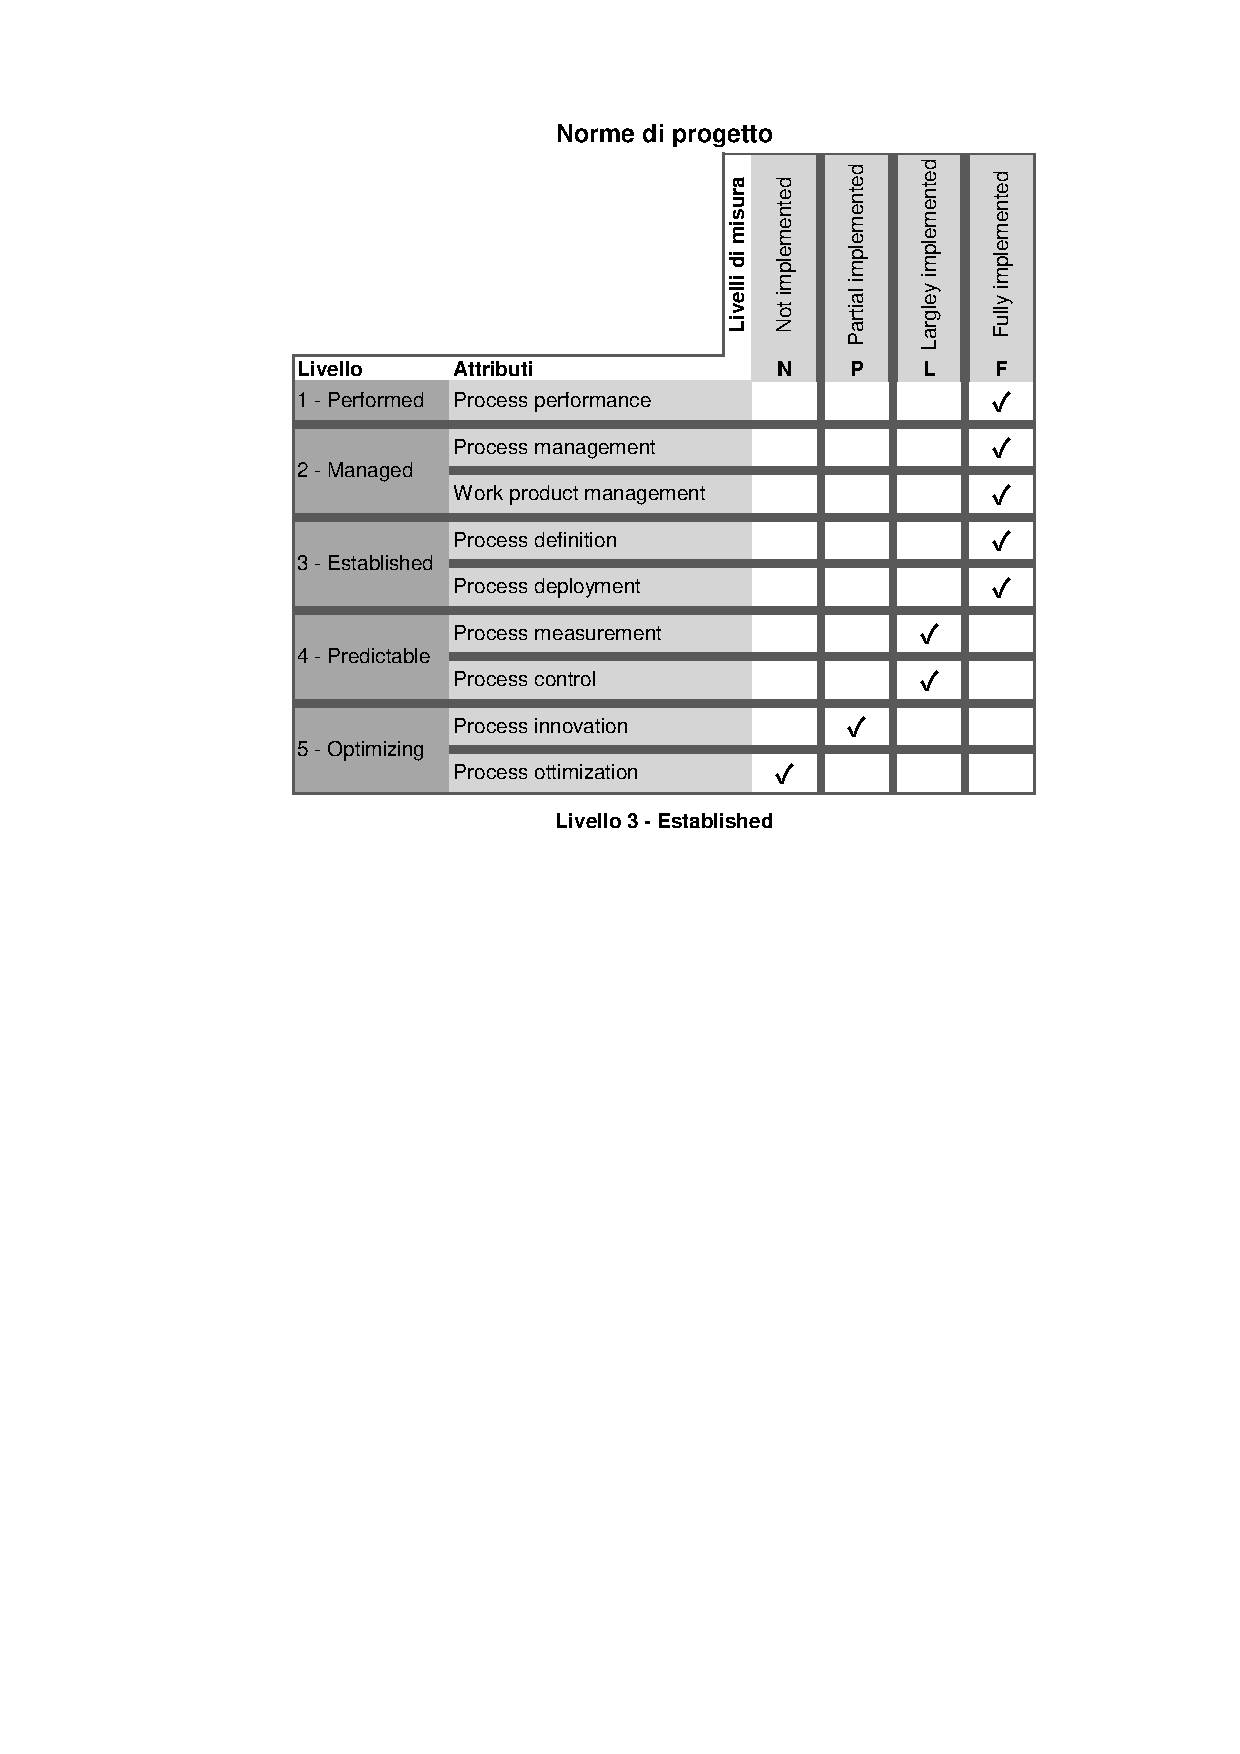
\includegraphics[scale=1]{images/resoconto/RR/normediprogetto-RR.pdf}
	\caption{Valori ISO/IEC 15504 Norme di progetto}	
\end{figure}
\newpage
\subparagraph{Analisi dei requisiti}
\noindent
\begin{figure}[H]
	\centering
	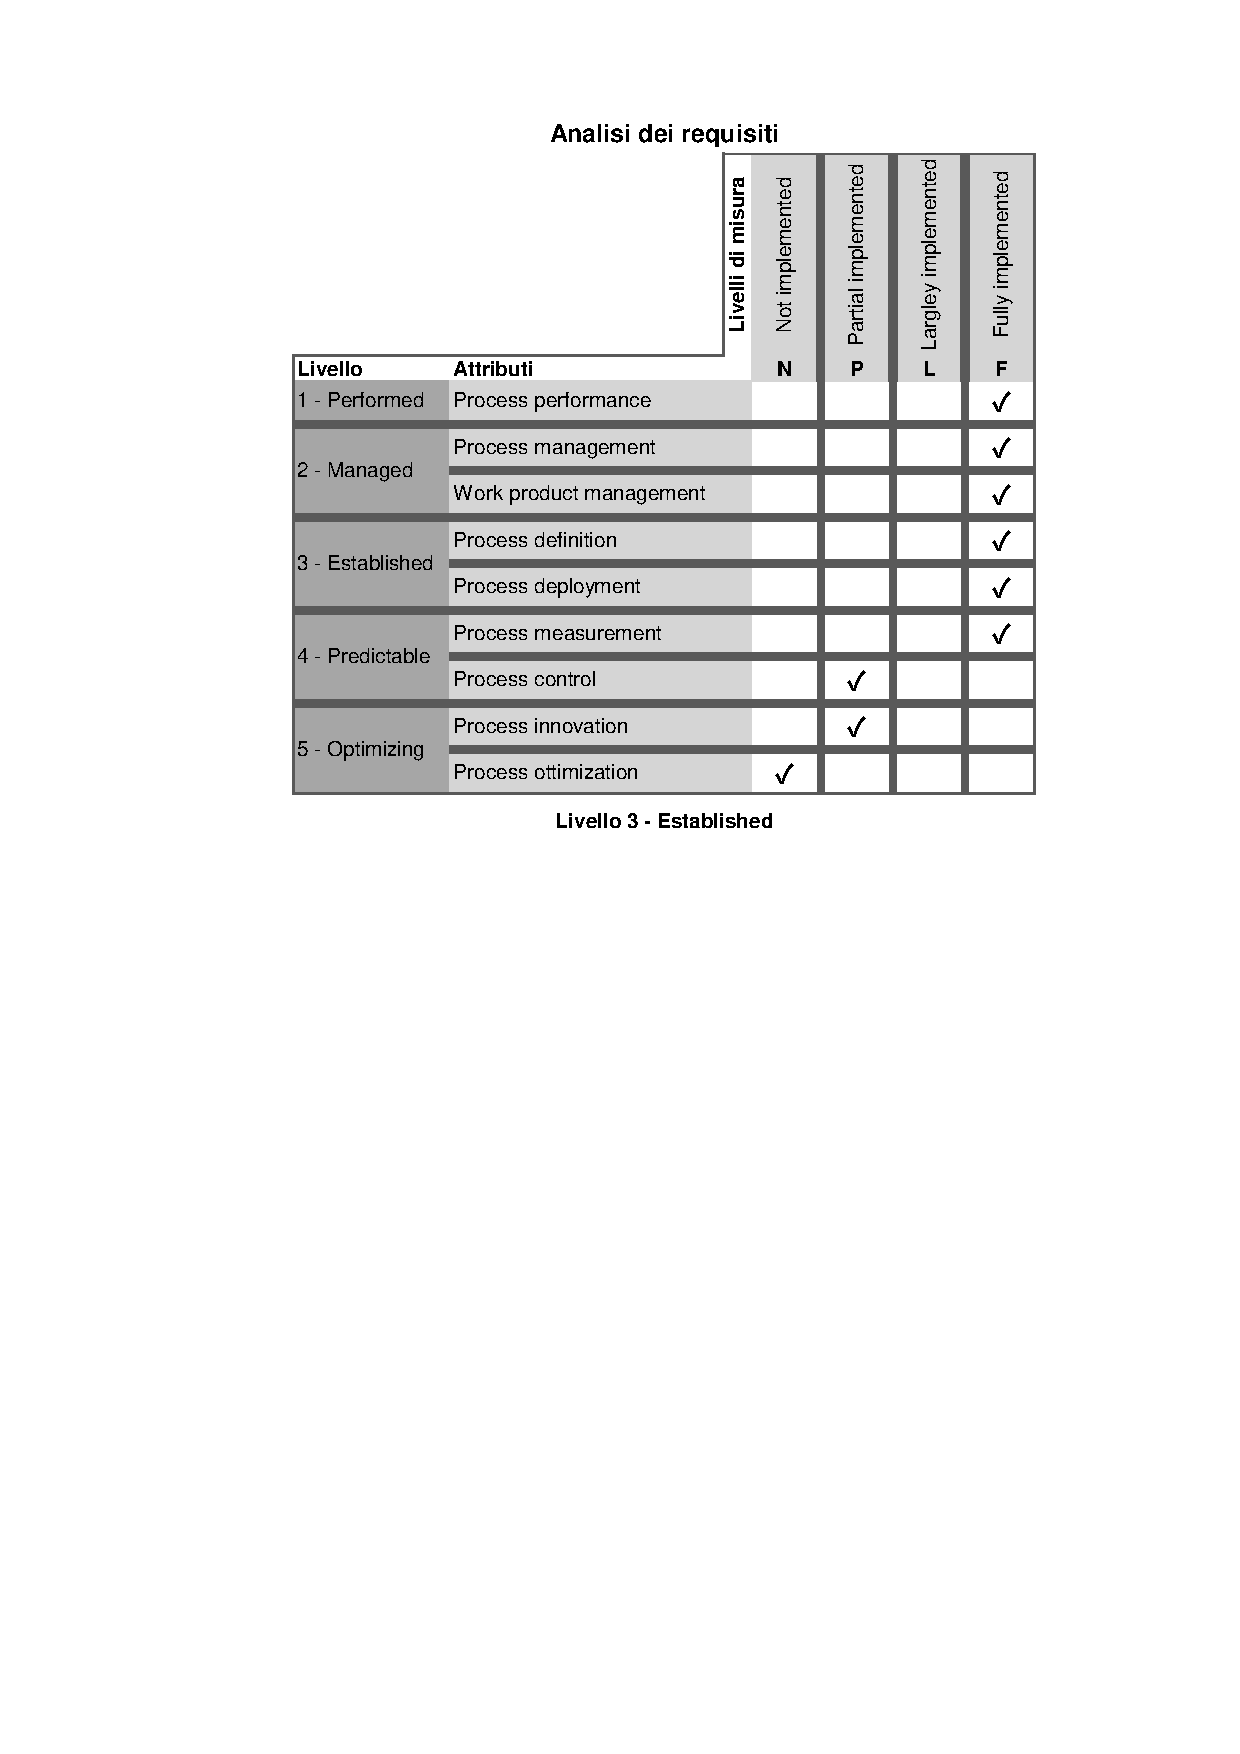
\includegraphics[scale=1]{images/resoconto/RR/analisideirequisiti-RR.pdf}
	\caption{Valori ISO/IEC 15504 Analisi dei requisiti}
\end{figure}
\newpage
\subparagraph{Pianificazione di progetto}
\noindent
\begin{figure}[H]
	\centering
	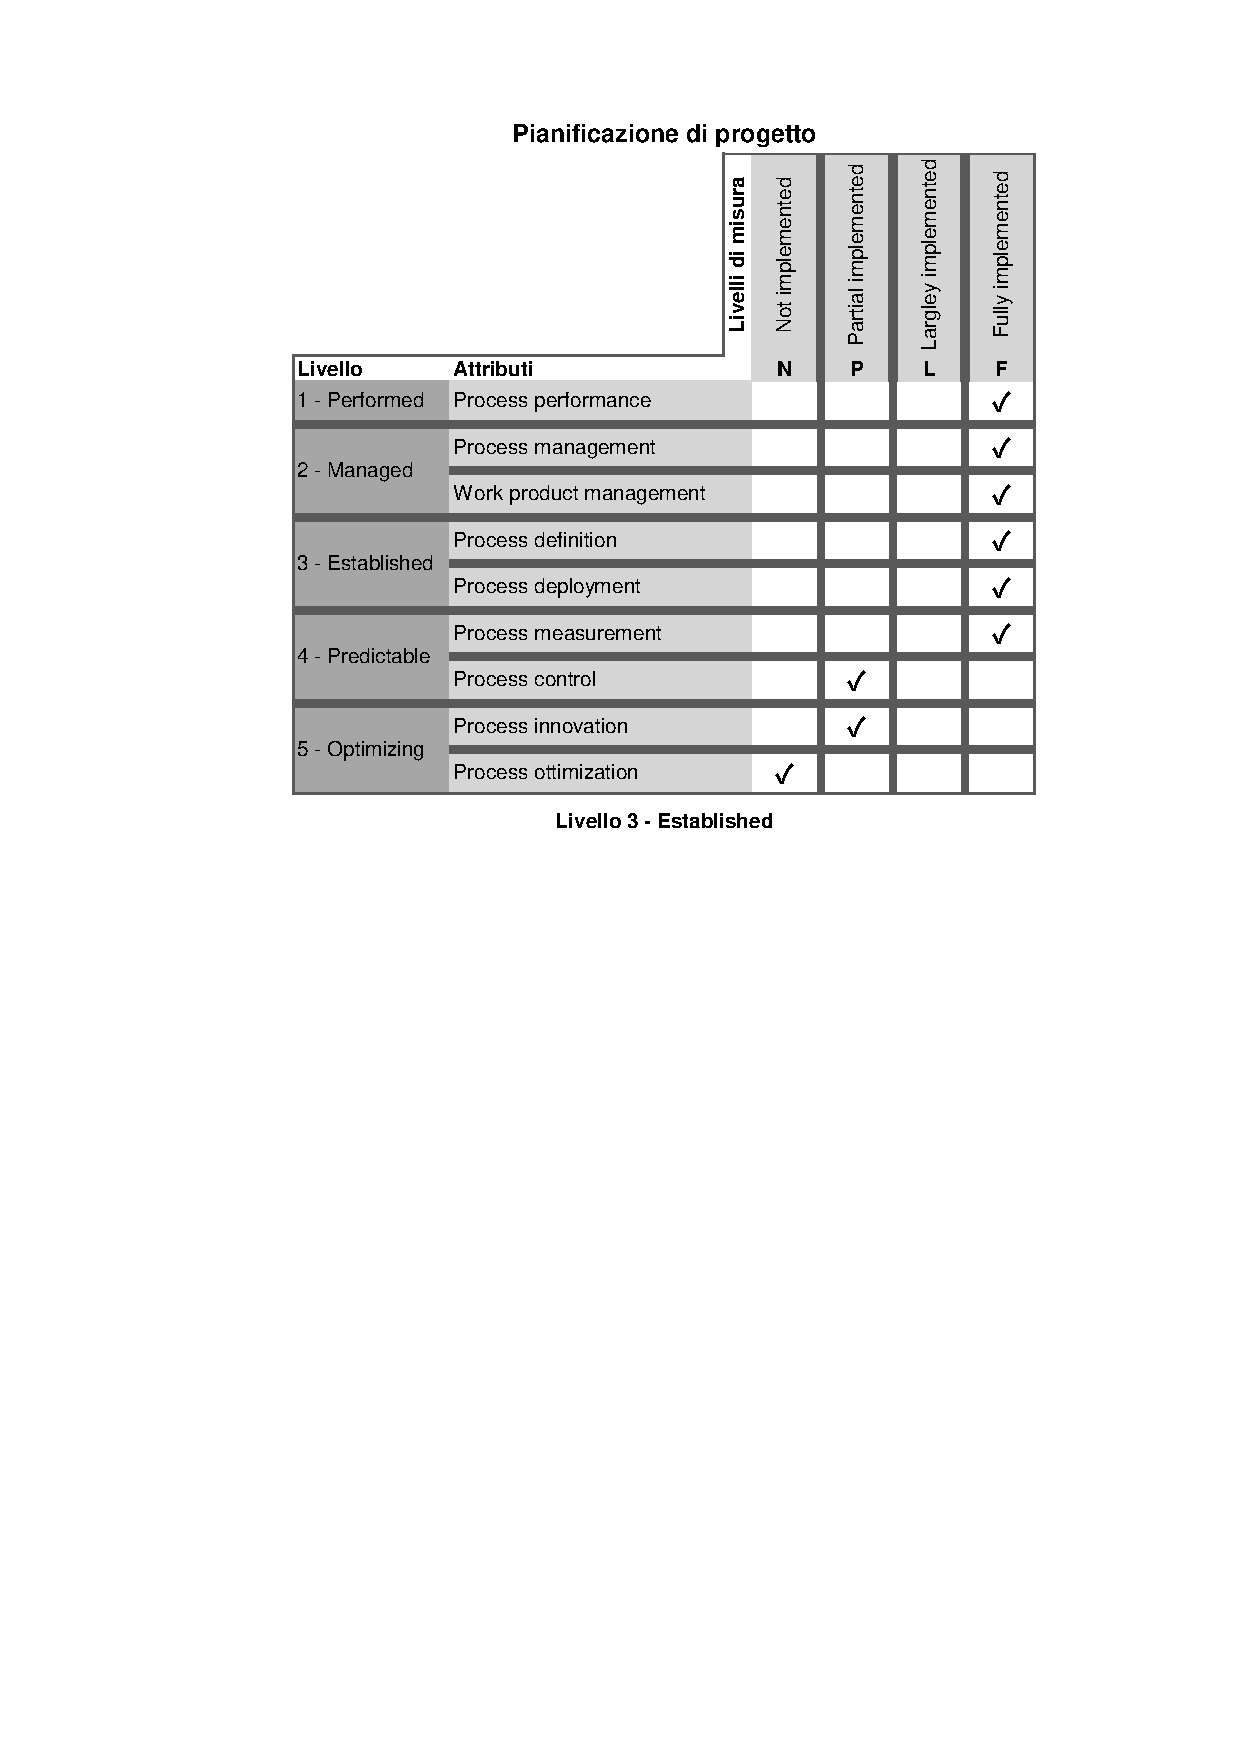
\includegraphics[scale=1]{images/resoconto/RR/pianificazioneprogetto-RR.pdf}
	\caption{Valori ISO/IEC 15504 Pianificazione di progetto}	
\end{figure}
\newpage
\subparagraph{Pianificazione di qualifica}
\noindent
\begin{figure}[H]
	\centering
	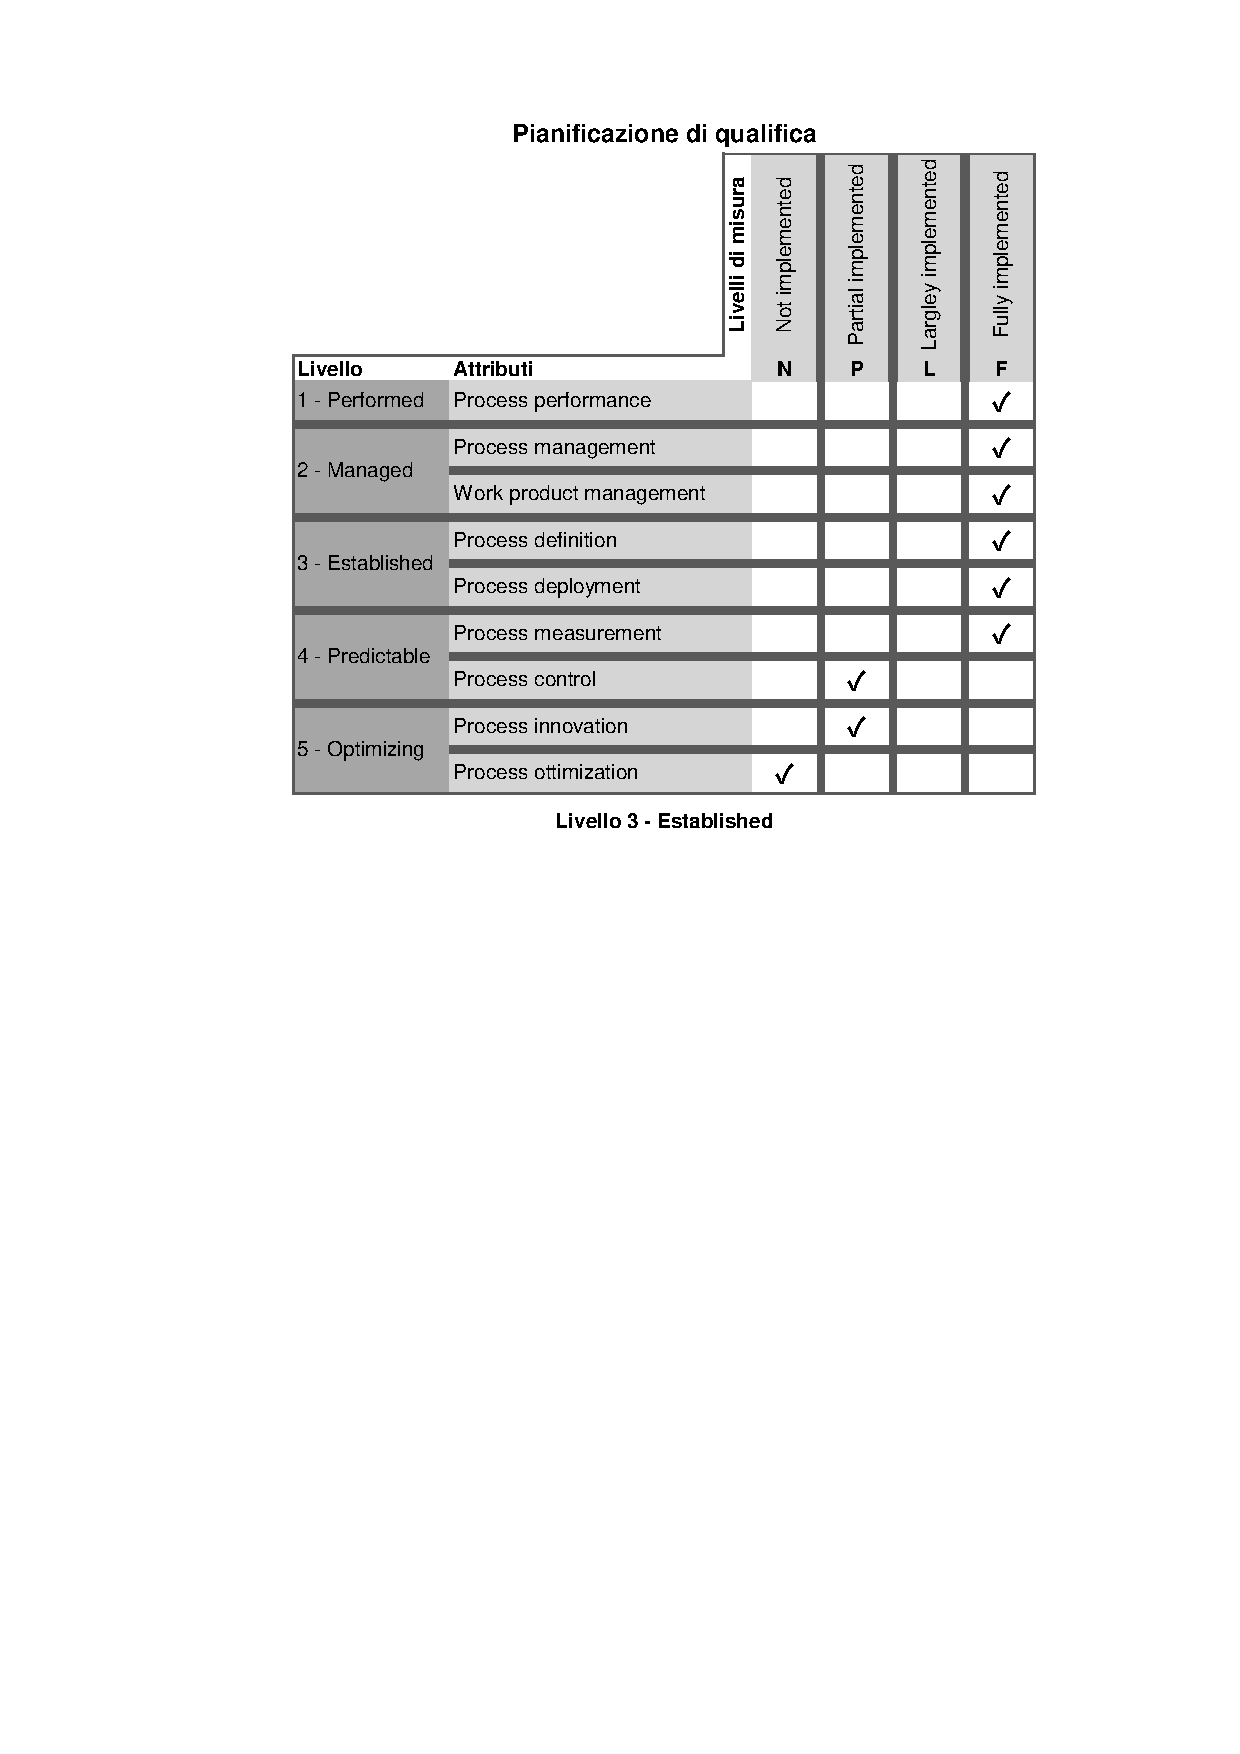
\includegraphics[scale=1]{images/resoconto/RR/pianificazionequalifica-RR.pdf}
	\caption{Valori ISO/IEC 15504 Pianificazione di qualifica}	
\end{figure}
\newpage

\subparagraph{Grafico riassuntivo}
Nel seguente grafico possiamo visualizzare una rappresentazione dei livelli raggiunti da ciascun processo implementato e quindi valutato durante il periodo della revisione dei requisiti. 

\begin{figure}[H]
	\centering
	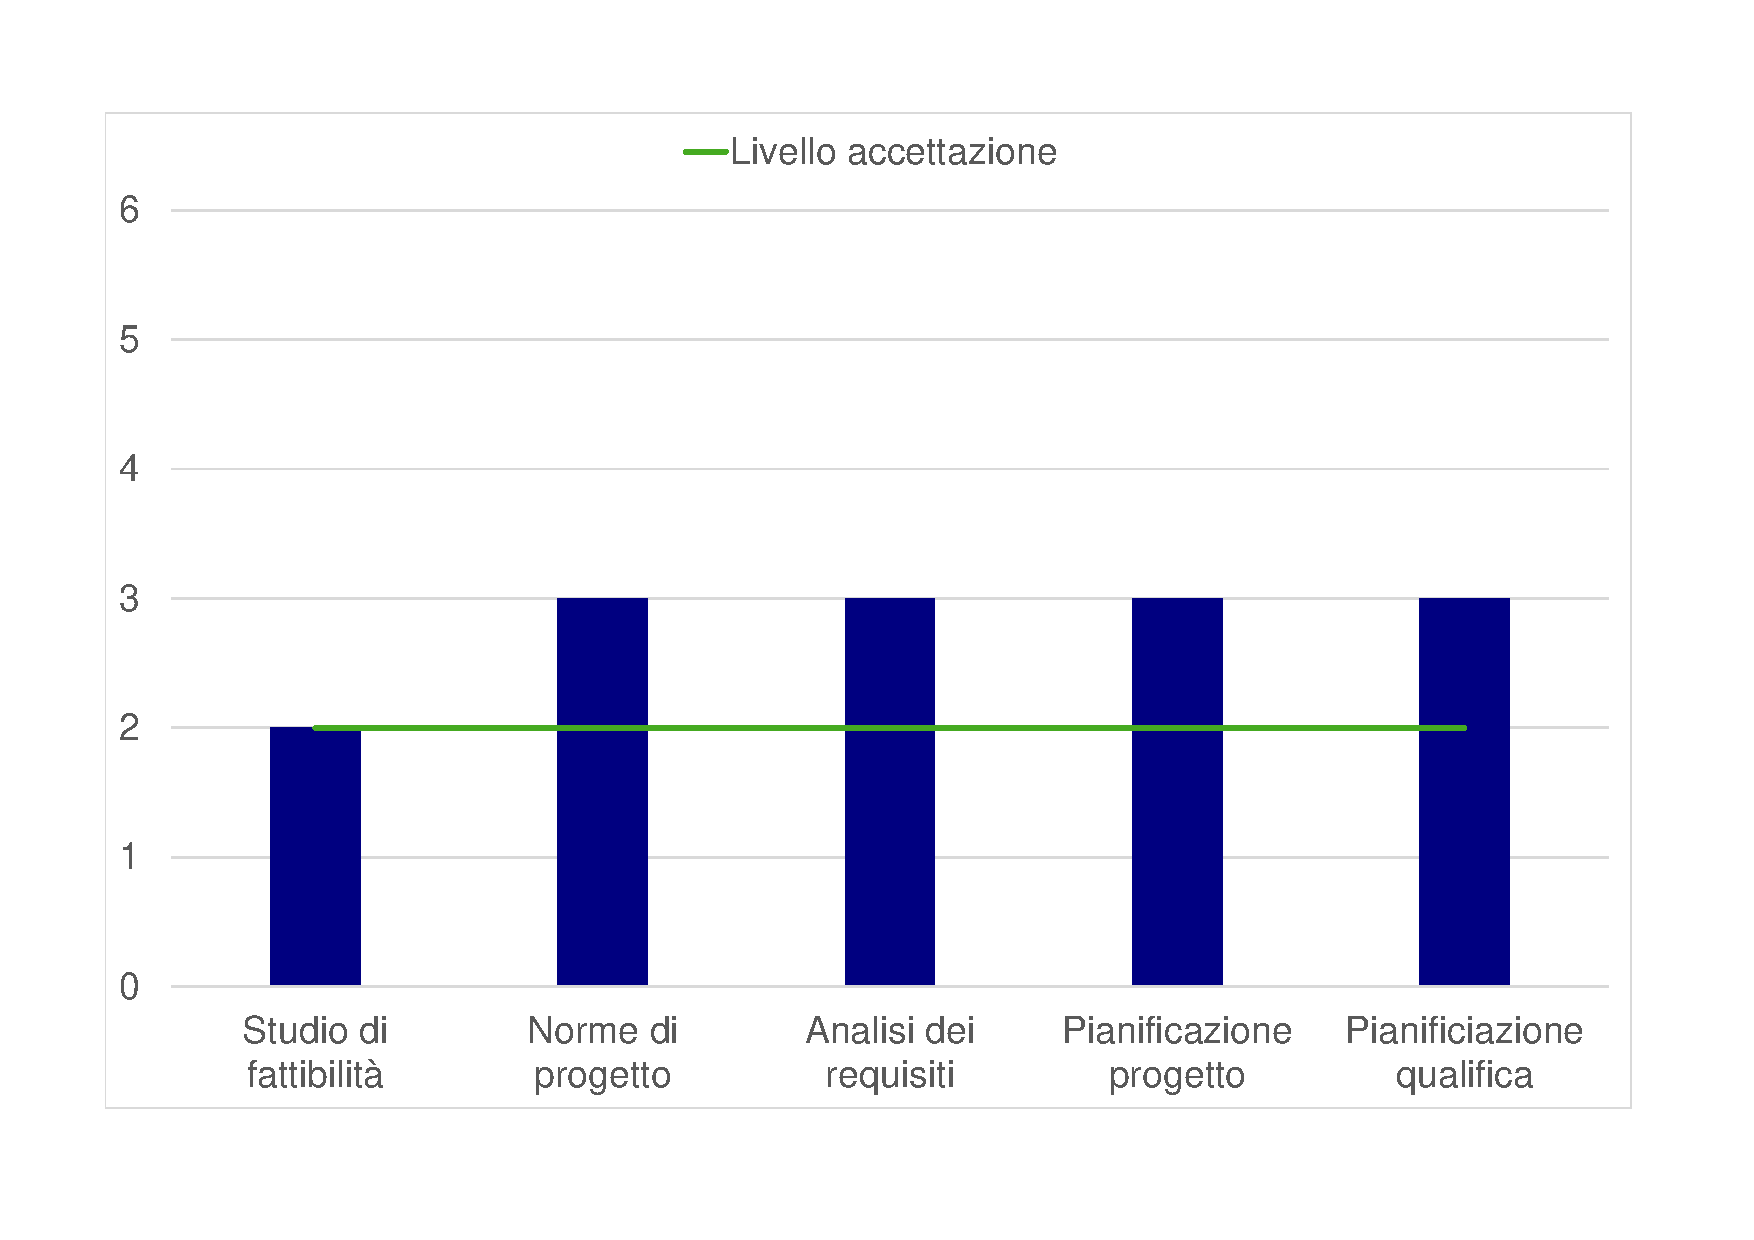
\includegraphics[scale=0.5]{images/resoconto/RR/chart-RR.pdf}
	\caption{Riassunto valori processi RR}
\end{figure}

\newpage
\paragraph{Revisione di Progettazione}
\noindent \\ 
Di seguito riportiamo le misurazioni dei processi più significativi sviluppati durante il periodo di Revisione di Progettazione. Tali valori sono stati raccolti secondo la metrica MPC1 che fa riferimento alle linee guida dettate dallo standard ISO/IEC 15504.
\subparagraph{Normazione}
\noindent
\begin{figure}[H]
	\centering
	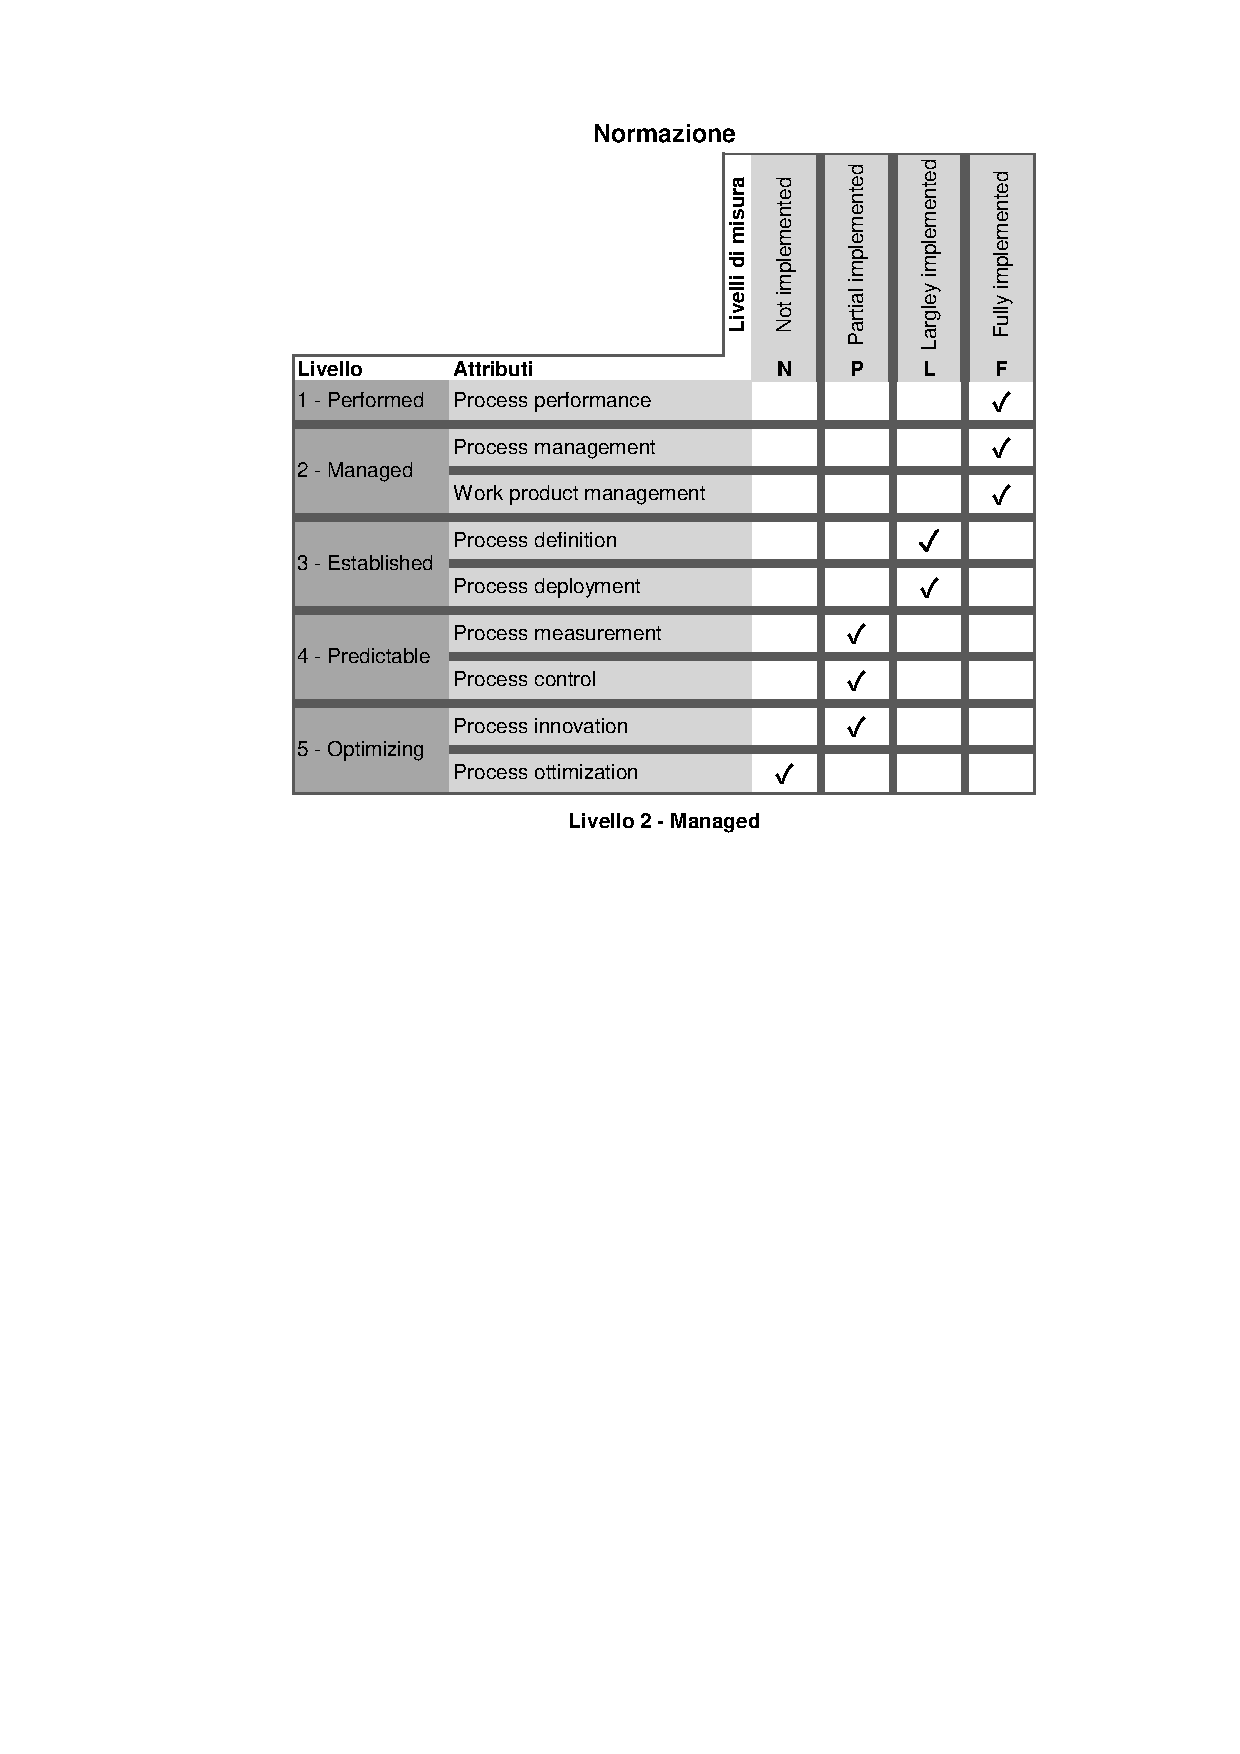
\includegraphics[scale=1]{images/resoconto/RP/normazione-RP.pdf}
	\caption{Valori ISO/IEC 15504 Pianificazione progetto}	
\end{figure}
\newpage
\subparagraph{Analisi dei requisiti}
\noindent
\begin{figure}[H]
	\centering
	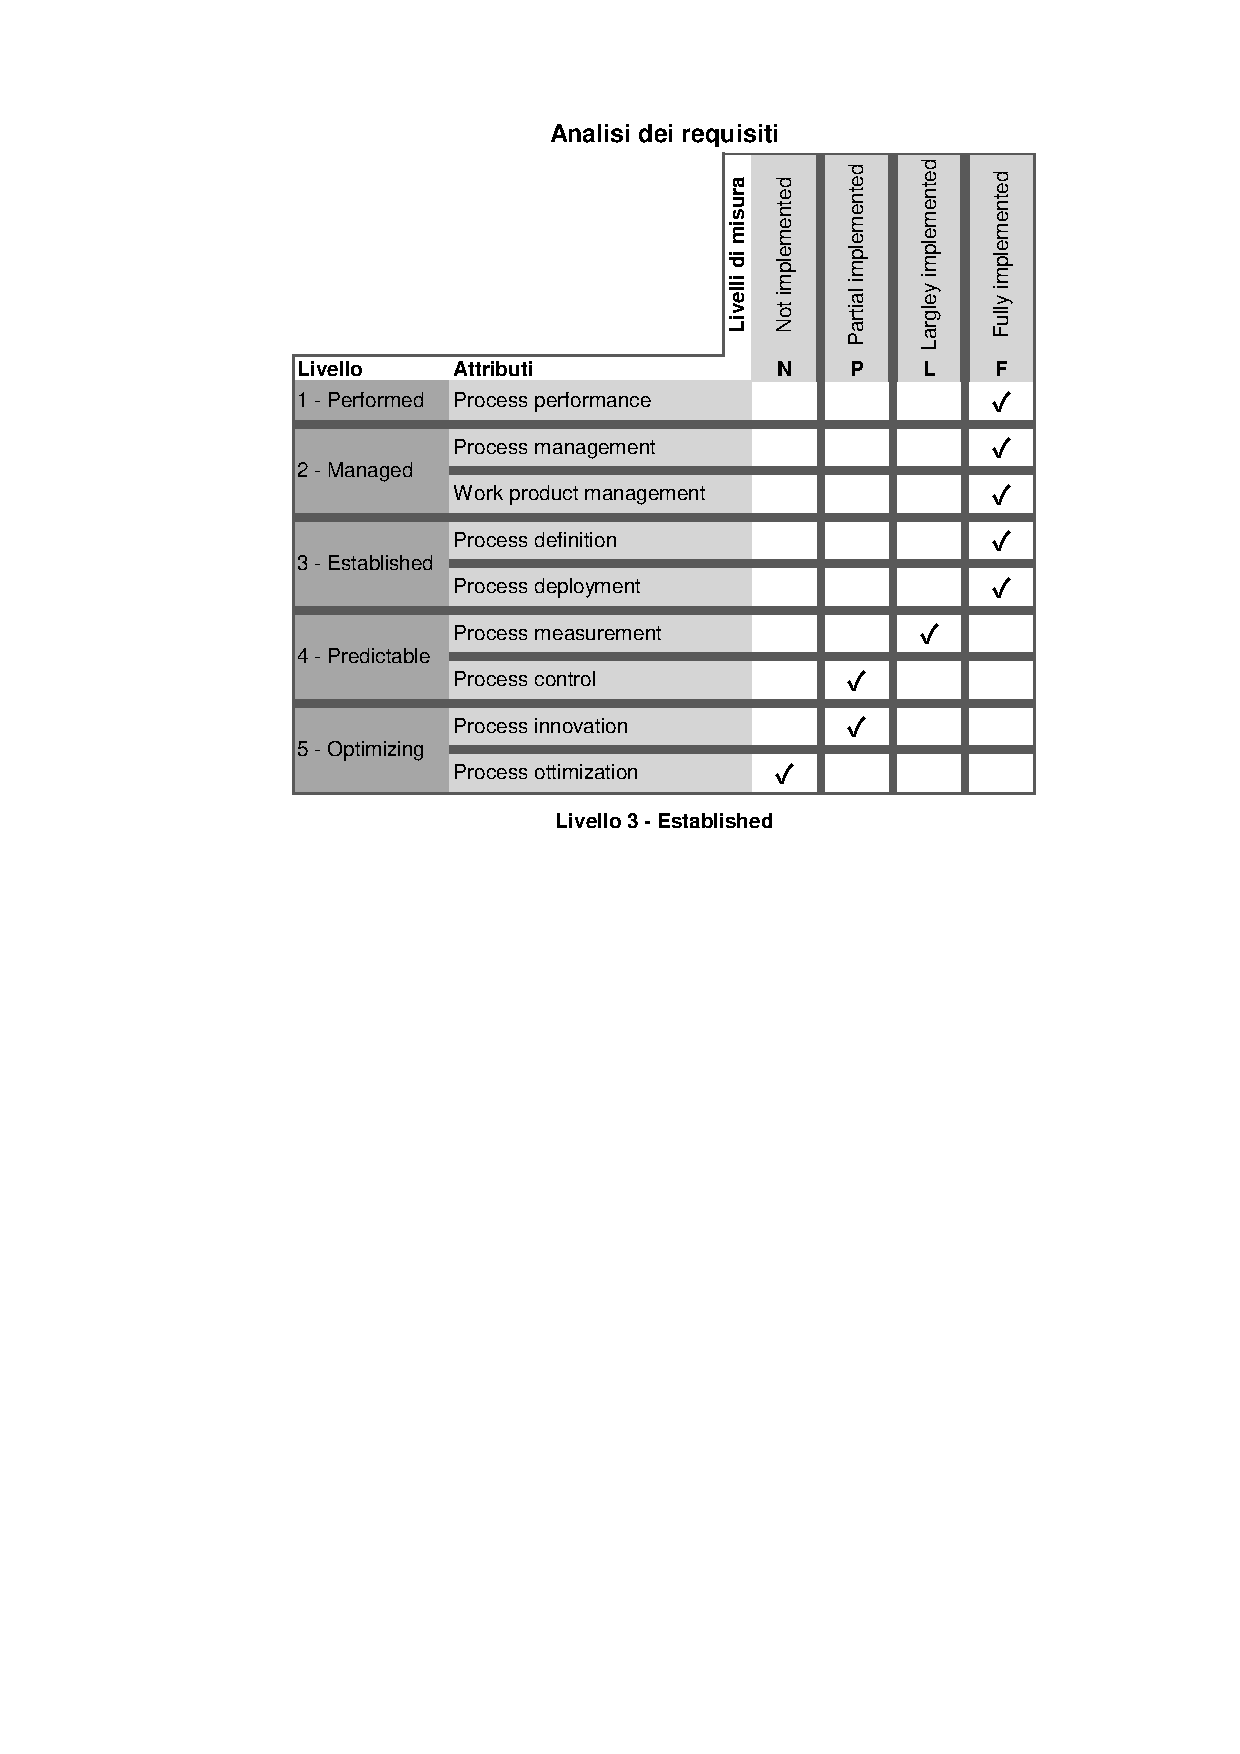
\includegraphics[scale=1]{images/resoconto/RP/analisideirequisiti-RP.pdf}
	\caption{Valori ISO/IEC 15504 Analisi dei requisiti}	
\end{figure}
\newpage
\subparagraph{Progettazione}
\noindent
\begin{figure}[H]
	\centering
	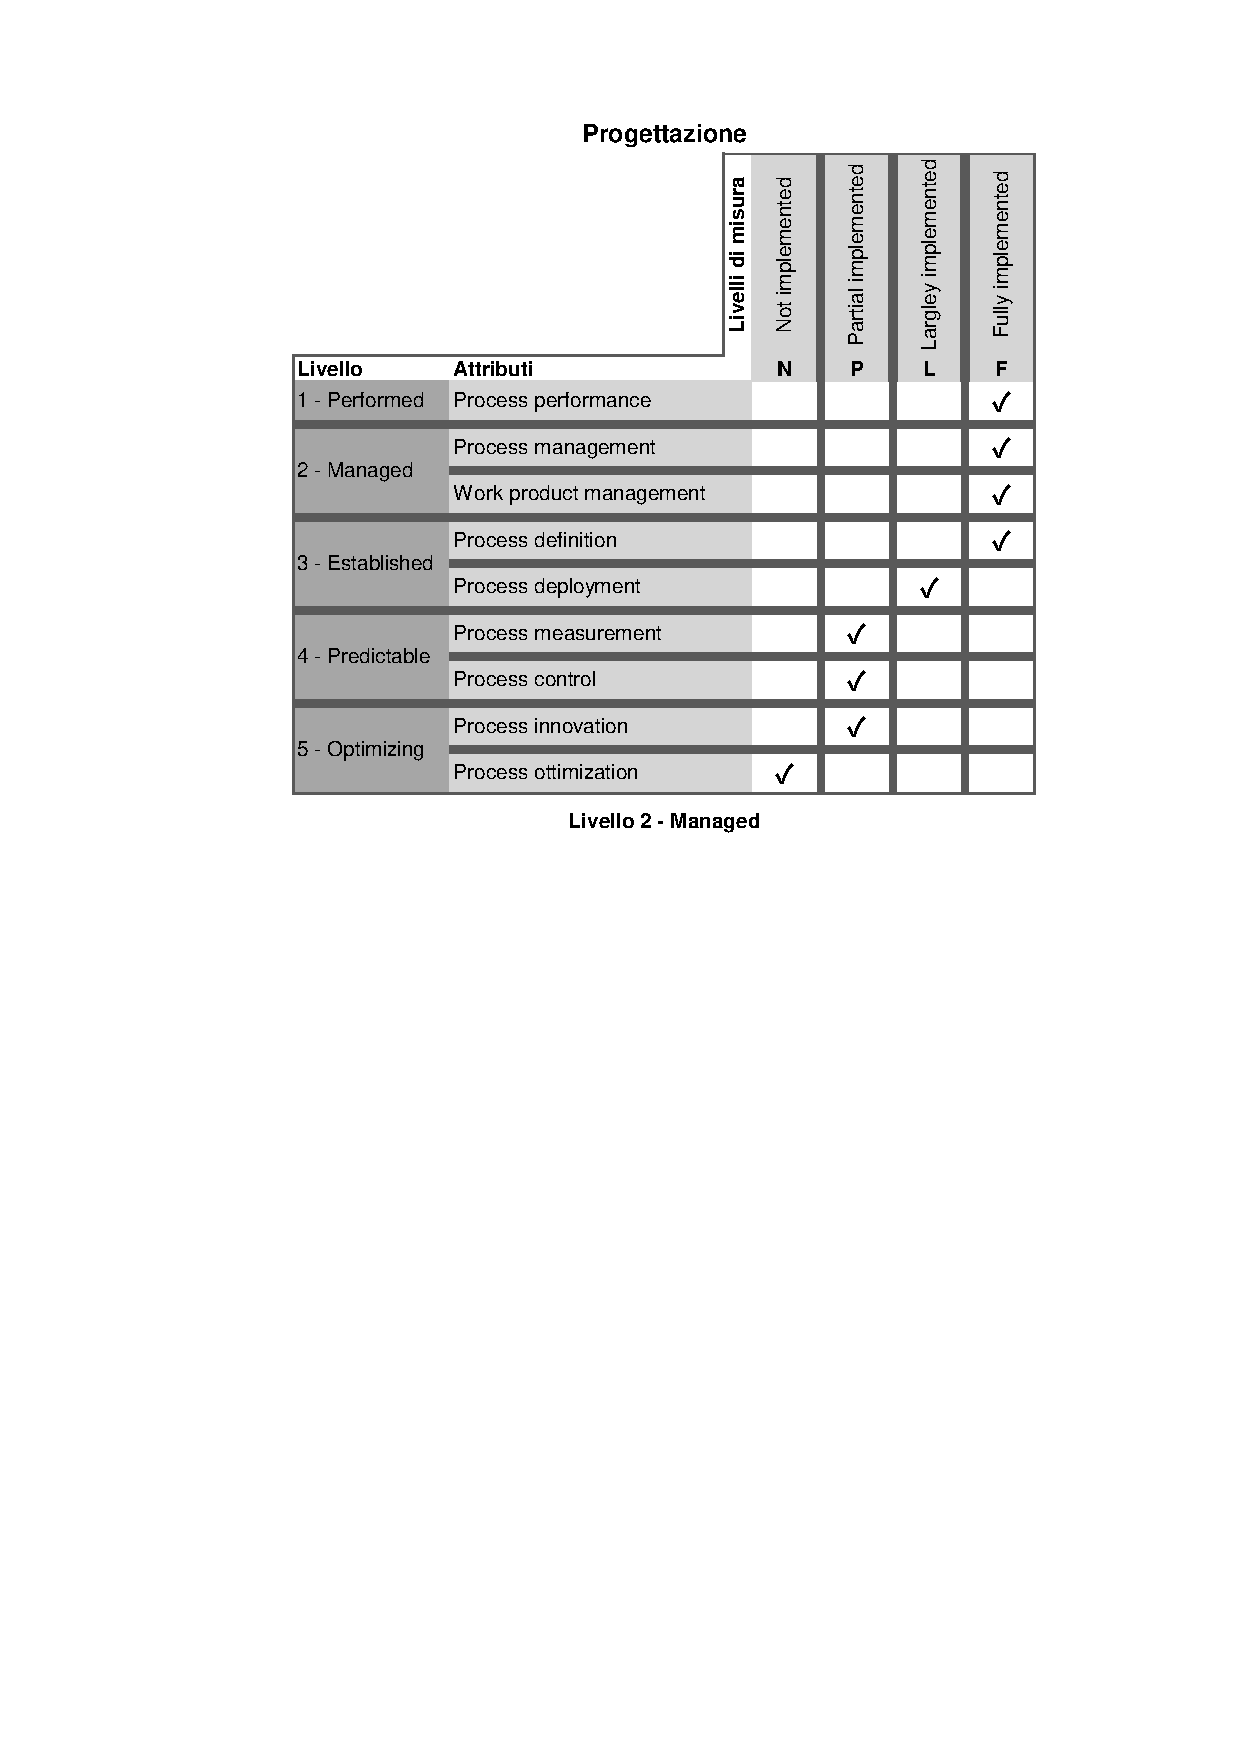
\includegraphics[scale=1]{images/resoconto/RP/progettazione-RP.pdf}
	\caption{Valori ISO/IEC 15504 Progettazione}	
\end{figure}
\newpage
\subparagraph{Documentazione}
\noindent
\begin{figure}[H]
	\centering
	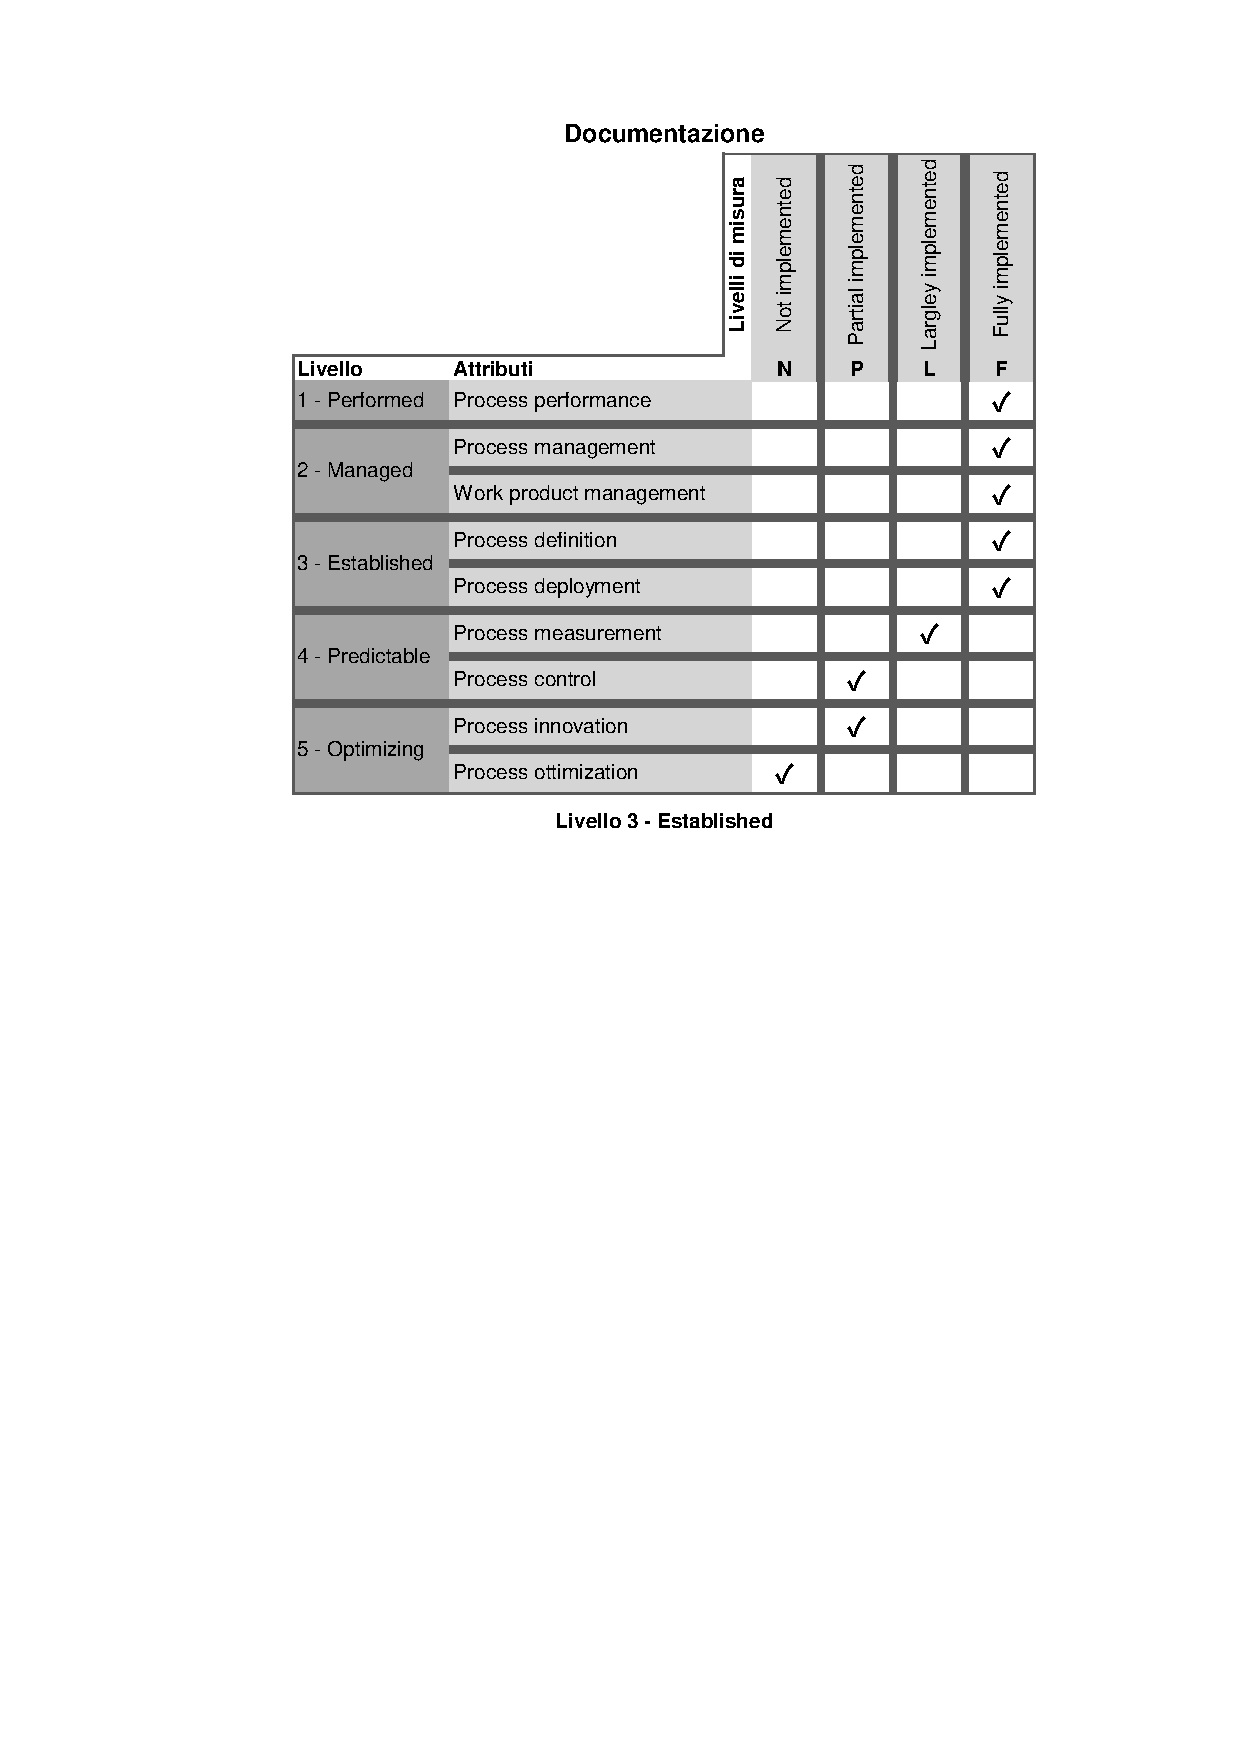
\includegraphics[scale=1]{images/resoconto/RP/documentazione-RP.pdf}
	\caption{Valori ISO/IEC 15504 Documentazione}	
\end{figure}
\newpage
\subparagraph{Pianificazione progetto}
\noindent
\begin{figure}[H]
	\centering
	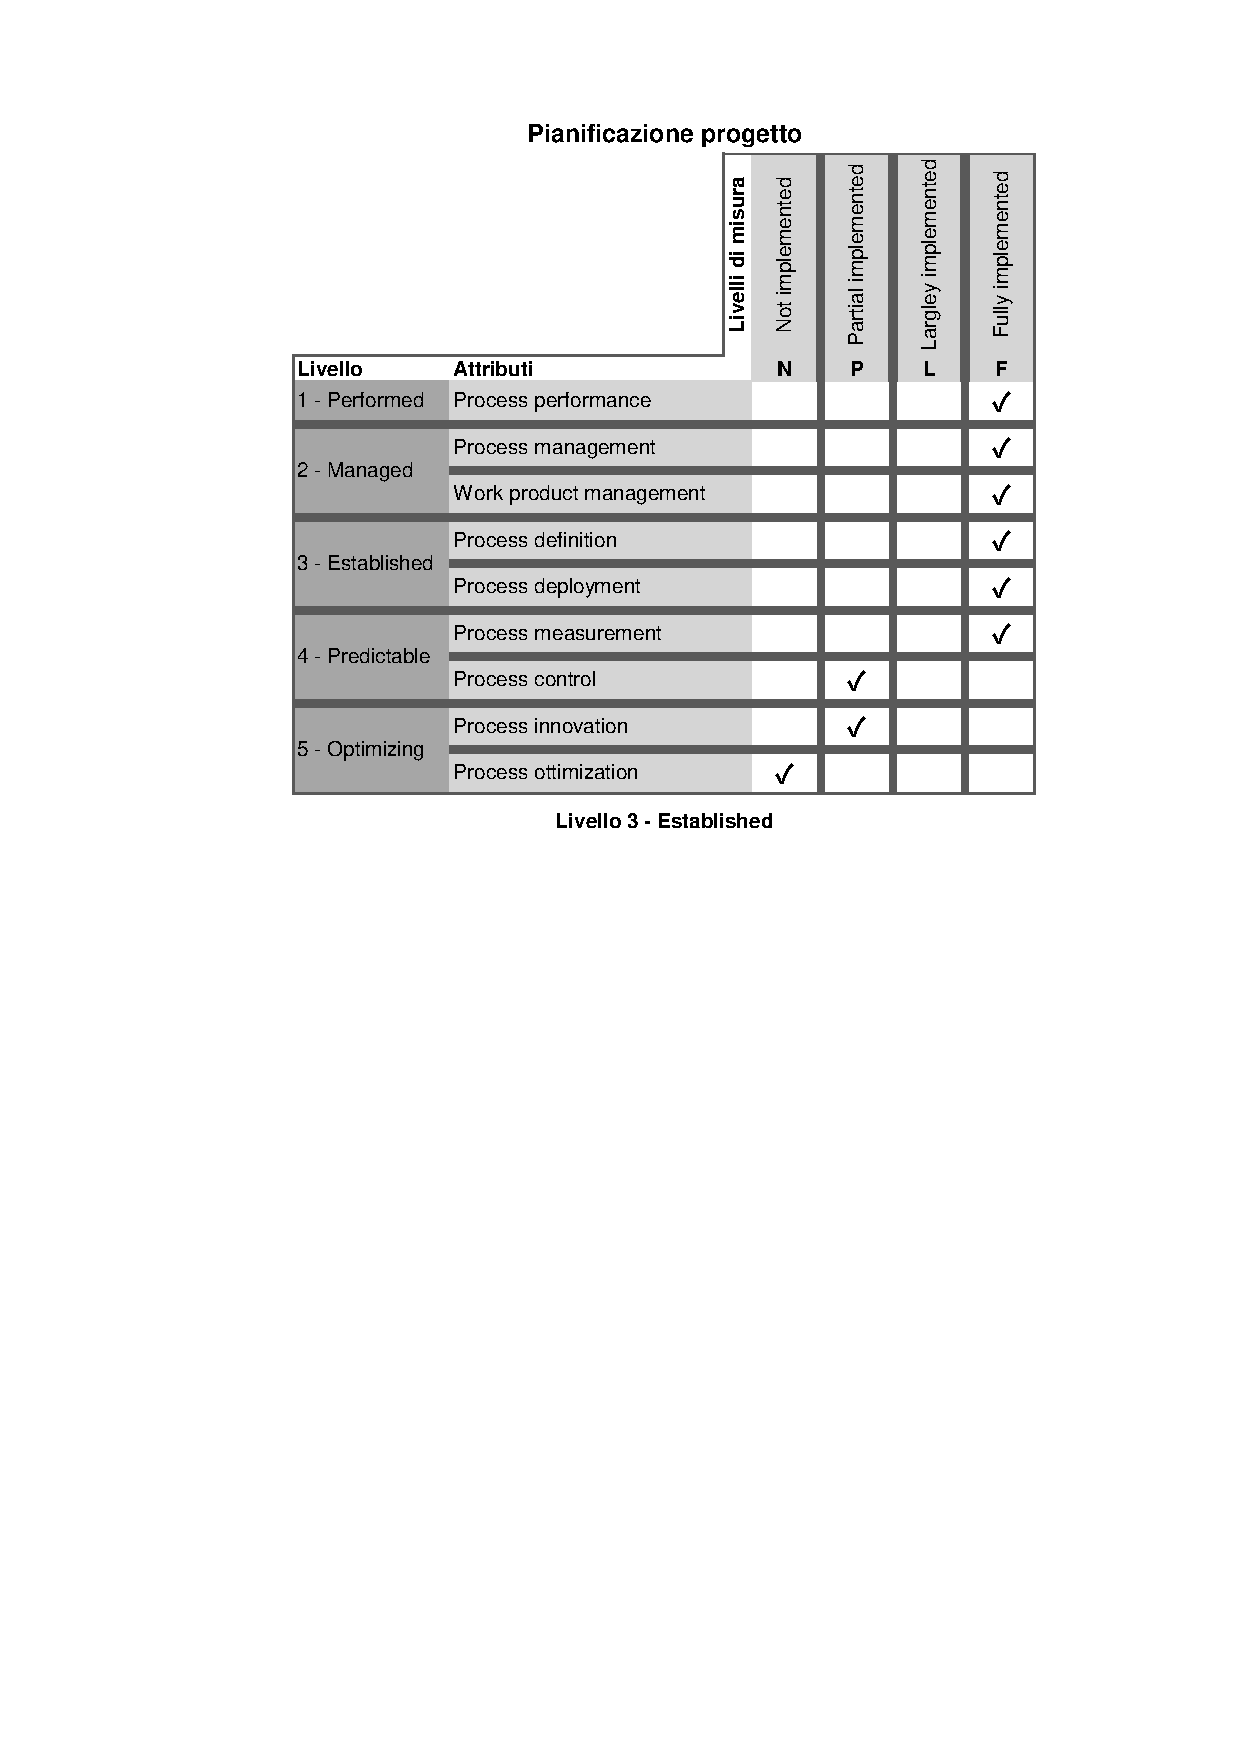
\includegraphics[scale=1]{images/resoconto/RP/pianificazioneprogetto-RP.pdf}
	\caption{Valori ISO/IEC 15504 Pianificazione progetto}	
\end{figure}
\newpage
\subparagraph{Ricerca delle tecnologie}
\noindent
\begin{figure}[H]
	\centering
	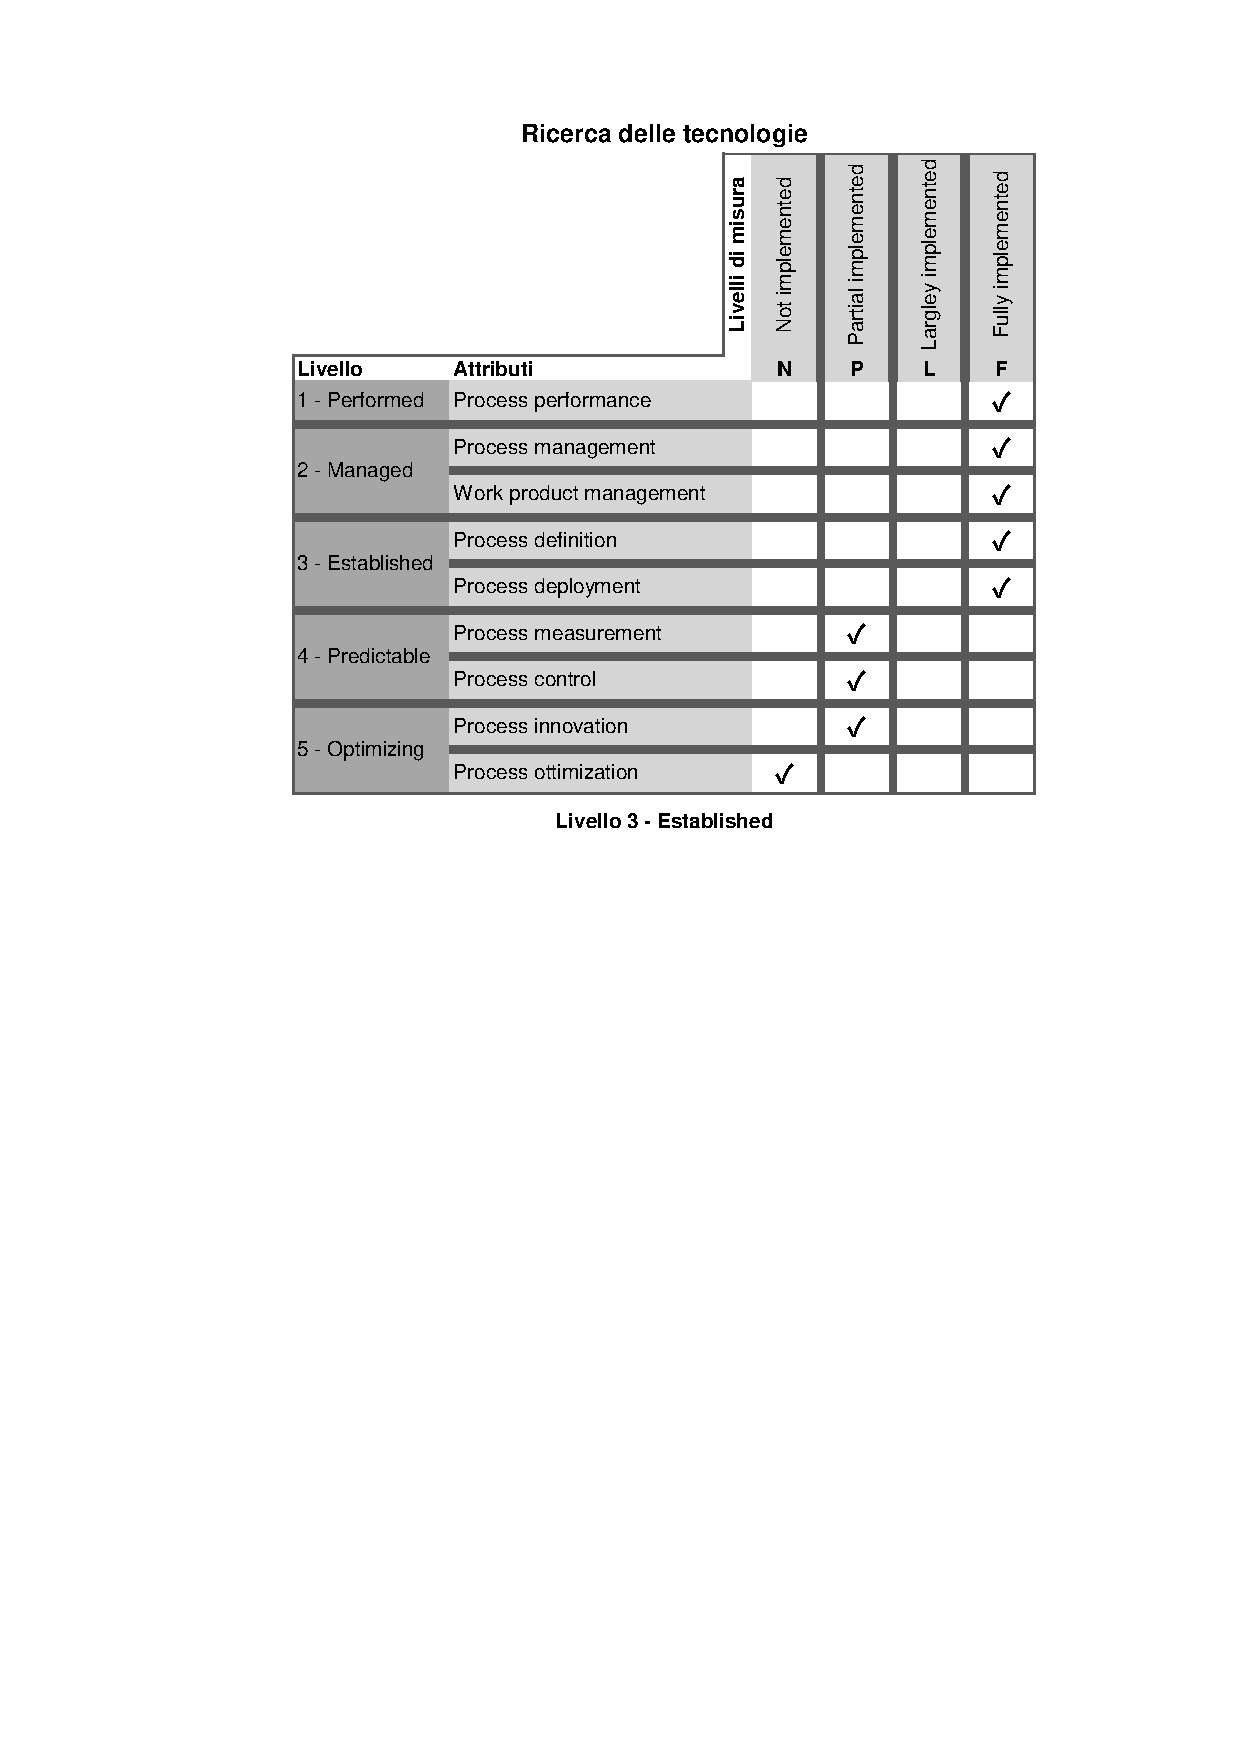
\includegraphics[scale=1]{images/resoconto/RP/ricercadelletecnologie-RP.pdf}
	\caption{Valori ISO/IEC 15504 Ricerca delle tecnologie}	
\end{figure}
\newpage

\subparagraph{Grafico riassuntivo}
Nel seguente grafico possiamo visualizzare una rappresentazione dei livelli raggiunti da ciascun processo implementato e quindi valutato durante il periodo della revisione di progetto. 

\begin{figure}[H]
	\centering
	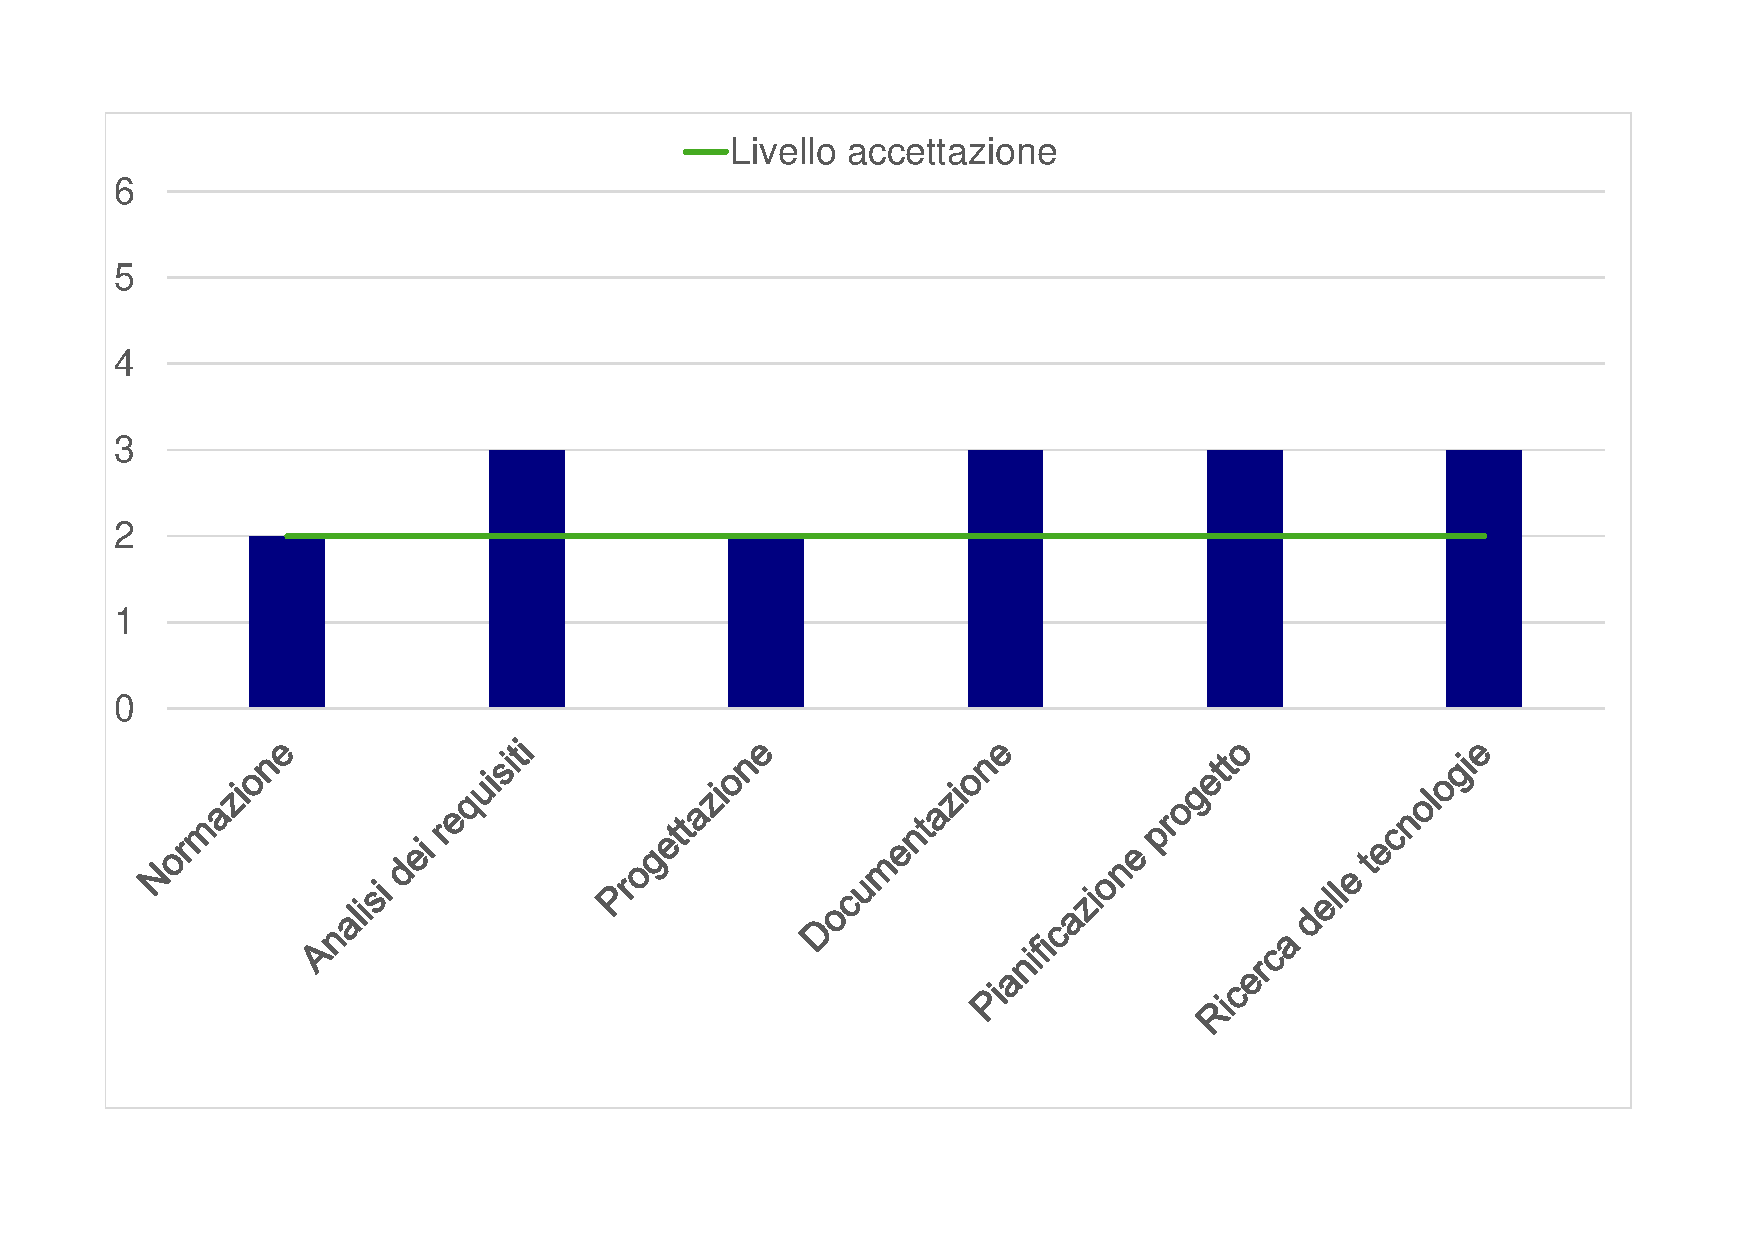
\includegraphics[scale=0.5]{images/resoconto/RP/chart-RP.pdf}
	\caption{Riassunto valori processi RP}	
\end{figure}

\newpage
\section{ISO/IEC 15504}
Lo standard ISO/IEC 15504, comunemente chiamato SPICE (acronimo di Software Process Improvement and Capability Determination), viene utilizzato per eseguire una valutazione concreta della qualità dei processi, inoltre permette la misurazione della capability dei processi, ovvero l'abilità con cui esso raggiunge l'obiettivo prefissato. Per eseguire queste misurazioni lo standard offre nove attributi da associare ai processi, ognuno dei quali misura un particolare aspetto della maturità del processo:
\begin{itemize}
	\item \textbf{Process performance:} è una misura del grado con cui è stato raggiunto lo scopo del processo. Il completo raggiungimento di quest'attributo è dato dal fatto che il processo raggiunge gli obiettivi prefissati.
	\item \textbf{Perfomance management:} è una misura del grado con il quale viene gestita l'organizzazione per il raggiungimento dello scopo del processo. Il processo è pianificato e monitorato. Le responsabilità per la realizzazione del processo sono assegnate e comunicate. Le risorse necessarie per il processo sono disponibili, allocate e utilizzate. 
	\item \textbf{Work product management:} è una misura del grado con il quale i risultati prodotti dal processo vengono appropriatamente gestiti. I requisiti dei risultati della documentazione e del controllo del processo sono definiti e i risultati devono essere appropriatamente documentati e controllati. I risultati del processo sono sottoposti a verifica e a correzione se necessario.
	\item \textbf{Process definition:} è una misura del grado con cui uno standard di processo è mantenuto (utilizzato) a supporto dell'implementazione del processo. Gli elementi fondamentali dello standard da utilizzare sono descritti e la sequenza di operazioni richieste dallo standard è definita. Le competenze, i ruoli, le infrastrutture e l'ambiente di lavoro per realizzare il processo fanno parte dello standard. I metodi di monitoraggio del processo sono definiti.
	\item \textbf{Process deployment:} è una misura del grado con il quale lo standard di processo viene effettivamente distribuito come un processo definito in grado di raggiungere i propri obiettivi. Le responsabilità e i ruoli per utilizzare lo standard sono assegnati e comunicati, le risorse, le infrastrutture e l'ambiente di lavoro, necessarie per l'applicazione dello standard, sono disponibili allocate e utilizzate. Vengono raccolti e analizzati dati per dimostrare l'adeguatezza e l'efficacia del processo.
	\item \textbf{Process measurement:} è una misura del grado con il quale i risultati delle misurazioni sono utilizzati per garantire il raggiungimento degli obiettivi del processo. Vengono definiti degli obiettivi di qualità basati sulle misurazioni. I risultati delle misurazioni sono raccolti analizzati e documentati per verificare che gli obiettivi di qualità siano rispettati.
	\item \textbf{Process control:} è una misura del grado con il quale il processo è quantitativamente gestito per produrre un processo che sia stabile, abile e previdibile entro limiti definiti. Analisi e tecniche di controllo vengono applicate. Sono stabiliti dei limiti di variazione per i risultati delle misurazioni. Vengono intraprese delle azioni correttive se necessario. 
	\item \textbf{Process innovation:} è una misura del grado con il quale vengono identificate delle modifiche al processo attraverso l'analisi di cause comuni di variazione delle performance, e dalla ricerca di approcci innovativi alla definizione e all'implementazione del processo. Vengono definiti degli obiettivi di miglioramento. Vengono analizzati dei dati per identificare le cause comuni di variazione delle performance del processo e sucessivamente per identificare delle best-practice*.
	\item \textbf{Process optimization:} è una misura del grado con il quale delle modifiche alla definizione, gestione e alle prestazioni del processo si traducono in un impatto che porta a raggiungere rilevanti miglioramenti al processo. L'impatto dei cambiamenti proposti viene valutato rispetto agli obiettivi definiti dal processo e dallo standard di processo.
\end{itemize}
A questi attributi viene assegnato uno dei seguenti quattro livelli di misura:
\begin{itemize}
	\item \textbf{N not implemented:} non ci sono segni di raggiungimento dell'attributo.
	\item \textbf{P partial implemented:} esistono alcuni risultati dell'attributo in questione.
	\item \textbf{L largely implemented:} ci sono significanti segni di raggiungimento dell'attributo in questione.
	\item \textbf{F fully implemented:} viene identificato un pieno raggiungimento degli obiettvi dell'attributo
\end{itemize}
Infine sulla base delle valutazioni assegnate ad ogni attributo del processo, potrà essere valutato il grado complessivo di maturazione, il quale varierà sui seguenti sei valori:
\begin{itemize}
	\item \textbf{0 - Incomplete:} viene rilevato un fallimento generale nel conseguimento dell'obiettivo del processo. Non si identifica alcun prodotto o risultato. Un processo appartenente a questo livello non può essere associato ad alcun attributo.
	\item \textbf{1 - Performed:} lo scopo del processo è generalmente raggiunto, a prova di ciò sono identificabili dei prodotti risultanti dal processo. A questo livello il processo viene associato all' attributo Process performance.
	\item \textbf{2 - Managed:} il processo raggiunge dei risultati di qualità accettabile rispettando i tempi prestabiliti. Il risultato soddisfa tutti i requisiti e gli standard predefiniti. Un processo a questo livello è quindi gestito tramite pianificazione e controllo e correzione dei suoi risultati, i quali possono essere ritenuti sicuri. Gli attributi associati a questo livello sono process management e work product management.
	\item \textbf{3 - Established:} il processo è implementato, gestito mediante procedure ben definite basate sui buoni principi dell'ingegneria del software. Un processo appartenente a questo livello sarà in grado di raggiungere sempre gli stessi risultati. Process definition e process deployment sono gli attributi associabili a questo livello.
	\item \textbf{4 - Predictable:} il processo raggiunge i propri obiettivi all'interno di limiti di controllo definiti. La sostanziale differenza con il livello estabilished è che ora il processo è quantitativamente compreso e controllato. A questo livello vengono associati gli attributi process measurement e process control.
	\item \textbf{5 - Optimizing:} le attività del processo sono ottimizzate per affrontare bisogni progettuali presenti e futuri, il processo viene sottoposto a miglioramento continuo. Gli attributi associati a questo livello sono process innovation e process optimization.
\end{itemize}
\begin{figure}[htbp]
	\centering
	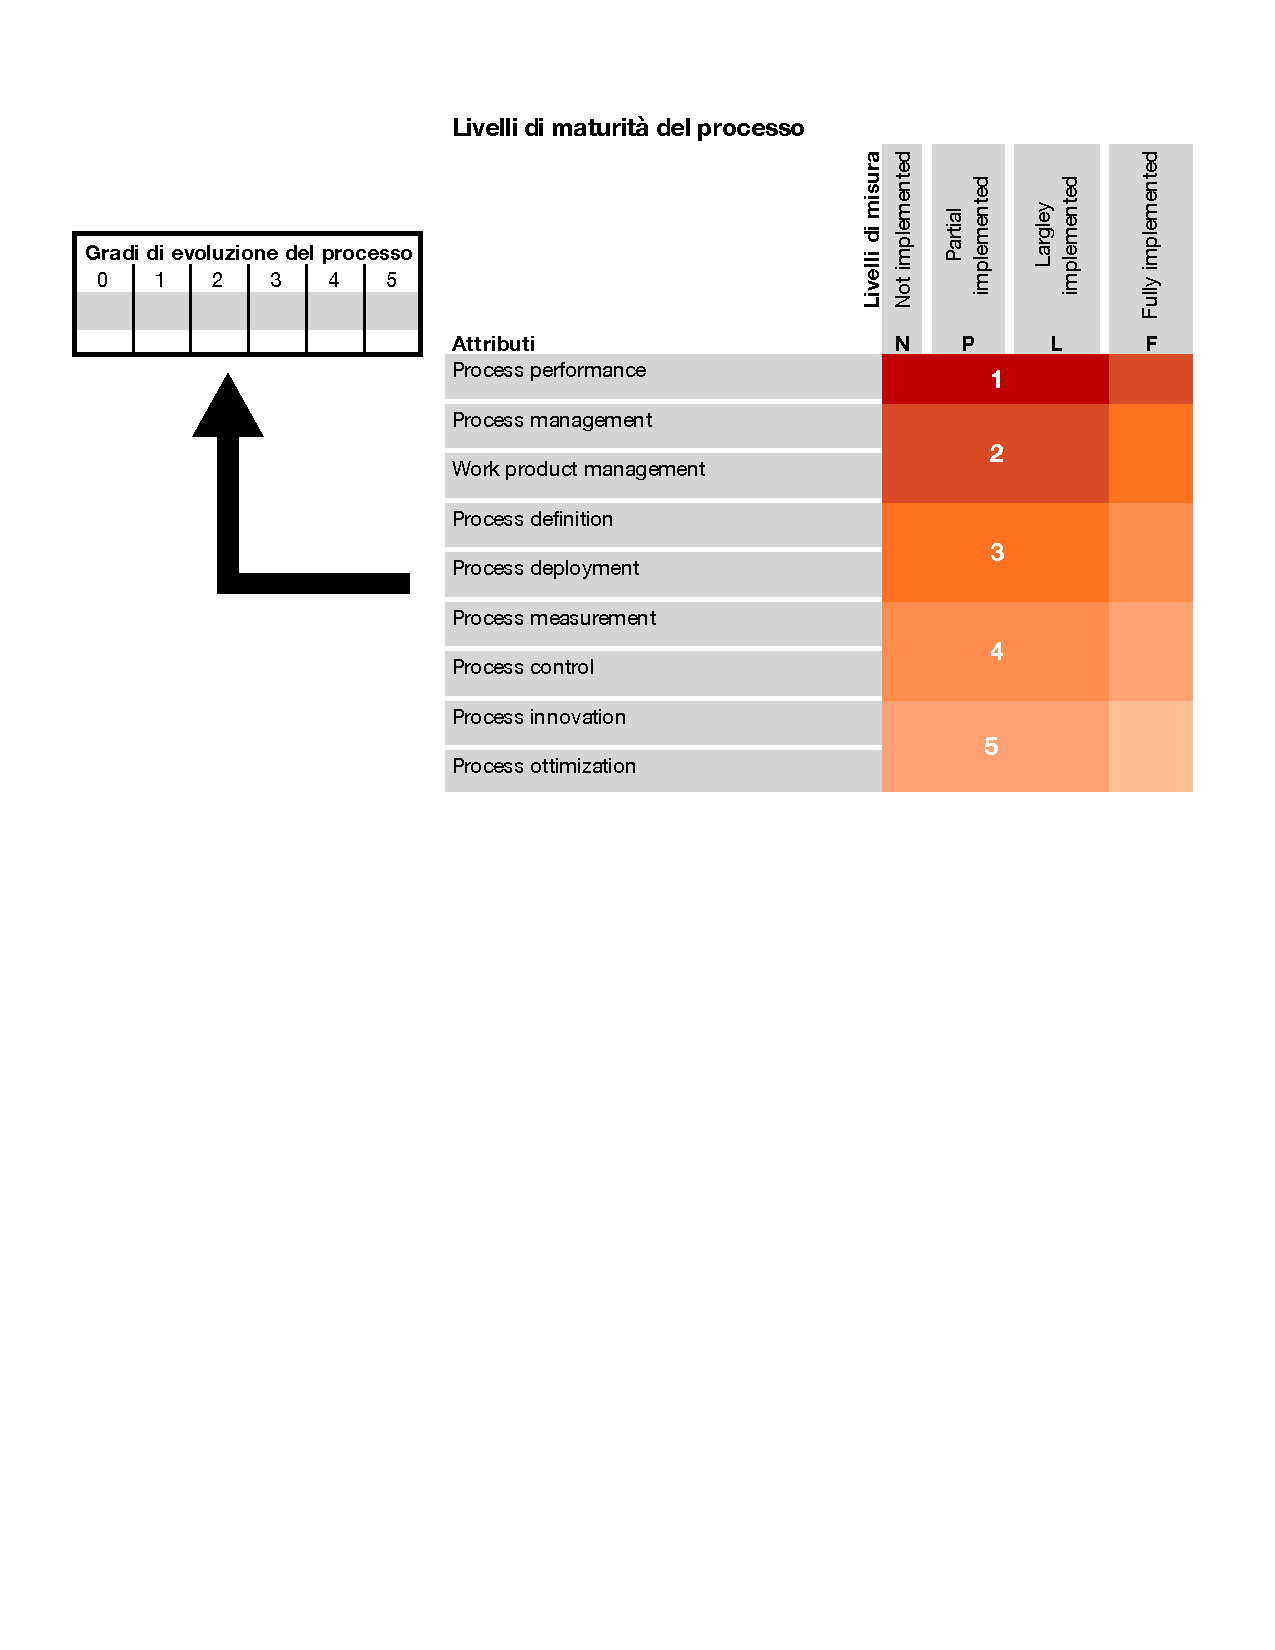
\includegraphics[scale=0.7]{images/ISOIEC15504.pdf}
	\caption{Riepilogo modello ISO/IEC 15504}
\end{figure}
\newpage

\subsection{Ciclo di Deming}
Il ciclo di Deming, noto anche come PDCA (dall'inglese \textbf{P}lan-\textbf{D}o-\textbf{C}heck-\textbf{A}ct), è un metodo di gestione iterativo suddiviso in quattro stadi ed utilizzato per il controllo del miglioramento continuo dei processi e dei prodotti. Esso permette, nello specifico, di migliorare gradualmente la qualità dei processi in termini di efficienza ed efficacia, ottimizzando l'uso delle risorse e misurando la loro conformità rispetto le aspettative. \\
La seguente immagine riporta le attività previste a tale scopo e ne segue una breve descrizione. 
\begin{figure}[htbp]
	\centering
	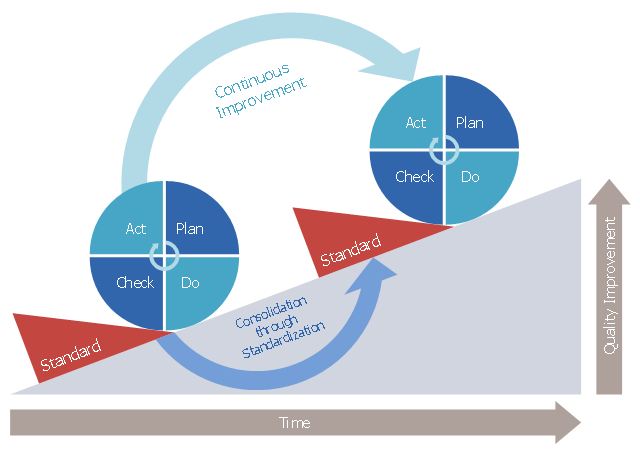
\includegraphics[scale=0.5]{images/pdca.png}
	\caption{Principio del miglioramento continuo secondo PDCA}
	
\end{figure}

\begin{itemize}
	\item \textbf{Plan}: prevede la definizione delle attività, scadenze, responsabilità e risorse atti a raggiungere e soddisfare degli obiettivi di miglioramento;
	\item \textbf{Do}: prevede l'esecuzione delle attività pianificate durante il periodo di pianificazione;
	\item \textbf{Check}: prevede la verifica dell'esito del processo in seguito all'attuazione delle strategie di miglioramento ed il confronto tra i risultati raccolti durante la fase Do e quelli attesi (specificati nella fase Plan) per stimare l'impatto effettivo del o dei miglioramenti apportati;
	\item \textbf{Act}: prevede l'attuazione delle strategie che hanno portato a dei miglioramenti. Nel caso i risultati attuali si distacchino da quelli previsti, si possono compiere delle azioni di correzione in seguito ad un'approfondita analisi delle cause di tale errore. 
\end{itemize}

\newpage
\section{ISO/IEC 9126}
Lo standard ISO/IEC 9126 definisce un modello dei requisiti qualitativi del Prodotto.
Il modello descritto si concentra in primo luogo sui tre punti di vista della qualità che esistono sul prodotto:
\begin{itemize}
	\item \textbf{Qualità esterna:} esprime il comportamento dinamico del software, in un determinato ambiente d'uso. In sostanza consiste nelle prestazioni e nelle funzionalità che il prodotto offre quando è in esecuzione;
	\item \textbf{Qualità interna:} esprime le proprietà statiche, cioè
	indipendenti dal contesto di esecuzione e uso. Sono direttamente misurabili ad esempio sul
	codice sorgente, pertanto senza la necessità di eseguire il software;
	\item \textbf{Qualità in uso:} esprime il livello con cui il prodotto si dimostra utile all'utente nel suo contesto d'uso. In altre parole rappresenta la capacità del prodotto di dare efficacia ed efficienza al lavoro dell'utente, a fronte di una sicurezza di utilizzo e di una soddisfazione nel far uso del prodotto.
\end{itemize}
\subsection{Modello per la qualità esterna ed interna}
Per la qualità esterna ed interna è definito un modello gerarchico formato da 6 caratteristiche principali e numerose sottocaratteristiche, tutte misurabili direttamente o indirettamente grazie all'utilizzo di metriche.
Le sei caratteristiche principali sono elencate di seguito:
\begin{itemize}
	\item \textbf{Funzionalità:} rappresenta la capacità del prodotto software di fornire funzioni che soddisfano le esigenze stabilite, sia esplicite che implicite, quando il software opera in un determinato contesto di utilizzo. Sottocaratteristiche notevoli sono l'interoperabilità e la Sicurezza, intesa come la capacità di proteggere le informazioni e i dati da accessi non autorizzati;
	\item \textbf{Affidabilità:} capacità di mantenere uno specificato livello di prestazione quando si opera in specificate condizioni. Sottocaratteristiche importanti sono la maturità e la tolleranza all'errore;
	\item \textbf{Efficienza:} capacità di fornire le funzioni richieste nel minor tempo possibile, sfruttando al meglio le risorse messe a disposizione;
	\item \textbf{Usabilità:} capacità del prodotto software di essere capito, appreso, usato e gradito all'utente, quando usato in contesti specificati. Una sottocaratteristica di rilievo è l'attrattiva;
	\item \textbf{Manutenibilità:} capacità del software di essere modificato e manutenuto. Per modifiche si intendono correzioni o adattamenti del software, negli ambienti, nei requisiti e nelle specifiche funzionali. Una sottocaratteristica importante è la testabilità, cioè la capacità di un software di consentire la verifica e di essere oggetto di test;
	\item \textbf{Portabilità:} capacità di poter essere trasferito da un ambiente di esecuzione all'altro.
\end{itemize}
\subsection{Modello per la qualità in uso}
Per la qualità in uso lo standard definisce una gerarchia separata, per enfatizzare il fatto che qui si considera non solo il prodotto software in sè, ma la relazione stretta tra esso e l'utente, nell'ambiente di utilizzo. Il modello è formato dalle seguenti quattro caratteristiche:
\begin{itemize}
	\item \textbf{Efficacia:} rappresenta la capacità di supportare un utente nel raggiungere i suoi obiettivi con accuratezza e completezza in un dato contesto;
	\item \textbf{Produttività:} la capacità di supportare un utente nello spendere l’appropriata quantità di risorse in relazione all’efficacia dei risultati da raggiungere; 
	\item \textbf{Soddisfazione:} la capacità di soddisfare un utente in un dato contesto d’uso;
	\item \textbf{Safety:} la capacità di raggiungere accettabili livelli di rischio di
	danni a persone, al software, ad apparecchiature, o all’ambiente operativo in un dato contesto d’uso.
\end{itemize}
\begin{figure}[htbp]
	\centering
	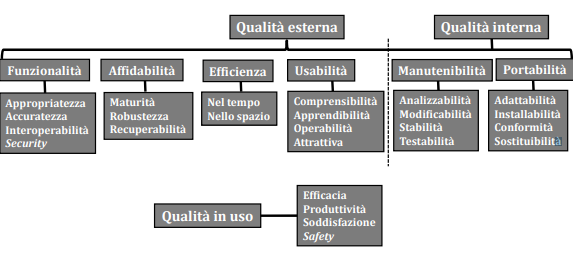
\includegraphics{images/gerarchiaQualitaProdotto.png}
	\caption{Riepilogo modello ISO 9126}
\end{figure}	
	\subsection{Test di integrazione}
Questa tipologia di test serve per verificare che le varie componenti del sistema interagiscono tra loro nella maniera attesa. La strategia per definire -e poi eseguire- i seguenti test, è quella di partire dalle singole componenti per poi realizzare le varie funzionalità incrementalmente durante lo sviluppo del prodotto finale. Questo potrà essere di aiuto in caso di errori, in quanto essi si presenteranno in un ambiente già testato e funzionante. \\
Per ogni test viene specificato il suo codice univoco, la descrizione e lo stato di implementazione attuale.

	\begin{longtable}{|>{\centering\arraybackslash}m{1.6cm}|>{\centering\arraybackslash}m{6.41cm}|>{\centering\arraybackslash}m{3.1cm}|}		
		\rowcolor{LightBlue}
		\textbf{\textcolor{white}{Test}}
		& \multicolumn{1}{|c|}{\textbf{\textcolor{white}{ Descrizione}}}\\
		\hline
		TI1
		& Test d’integrazione front-end e back-end per la corretta visualizzazione del front-end.
		\\ \hline
		\rowcolor{LightGray}
		TI2
		& Test d’integrazione front-end e back-end per l'invio dei dati al front-end.
		\\ \hline
		TI3
		& Test d’integrazione front-end e back-end per la ricezione di dati dal front-end tramite POST.
		\\ \hline
		\rowcolor{LightGray}
		TI4
		& Test d’integrazione front-end e back-end per la ricezione di dati dal front-end tramite GET.
		\\ \hline
		TI5
		& Test d’integrazione tra back-end e Hunpos per il POS-Tagging$^*$.
		\\ \hline
		\rowcolor{LightGray}
		TI6
		& Test d’integrazione tra back-end e Hunpos per il training.
		\\ \hline	
		TI7
		& Test d’integrazione tra back-end e Google Firebase Realtime Database per la lettura dalla base di dati.
		\\ \hline	
		\rowcolor{LightGray}
		TI8
		& Test d’integrazione tra back-end e Google Firebase Realtime Database per la scrittura sulla base di dati.
		\\ \hline	
		TI9
		& Test d’integrazione tra back-end e Google Firebase Realtime Database per la modifica della base di dati.
		\\ \hline	
		\rowcolor{LightGray}
		TI10
		& Test d’integrazione tra back-end e Google Firebase Realtime Database per l'eliminazione dalla base di dati.
		\\ \hline	
		\caption{Test di integrazione - descrizione}
\end{longtable}


\subsection{Test di unità}
\begin{longtable}{|>{\centering\arraybackslash}m{1.6cm}|>{\centering\arraybackslash}m{6.41cm}|>{\centering\arraybackslash}m{3.1cm}| c |}		
		\rowcolor{LightBlue}
		\textbf{\textcolor{white}{Test}}
		& \multicolumn{1}{|c|}{\textbf{\textcolor{white}{ Descrizione}}}\\
		\hline
		TU1 & Verifica che il metodo ritorni l'id corretto della classe su cui è richiamato. \\ \hline
		TU2 & Verifica che il metodo ritorni il nome corretto della classe su cui è richiamato. \\ \hline
		TU3 & Verifica che il metodo ritorni la descrizione corretta della classe su cui è richiamato.\\ \hline
		TU4 & Verifica che venga ritornato l'id corretto dell'insegnante creatore della classe su cui il metodo è richiamato. \\ \hline
		TU5 & Verifica che venga ritornata la corretta lista di studenti appartenenti alla classe su cui il metodo è richiamato.  \\ \hline
		TU6 & Verifica che venga ritornata la corretta lista di esercizi assegnati alla classe su cui il metodo è richiamato.\\ \hline
		TU7 & Verifica che ritorni il giusto numero di studenti studenti appartenenti alla classe su cui il metodo è richiamato.  \\ \hline
		TU8 & Verifica che il metodo elimini correttamente uno studente dalla lista di quelli appartenenti alla classe su cui è  richiamato.  \\ \hline
		TU9 & Verifica che il metodo elimini correttamente un esercizio dalla lista di quelli assegnati alla classe su cui è  richiamato.\\ \hline
		TU10 & Verifica che il metodo aggiunga correttamente uno studente dalla lista di quelli appartenenti alla classe su cui è  richiamato.\\ \hline
		TU11 & Verifica che il metodo aggiunga correttamente un esercizio dalla lista di quelli assegnati alla classe su cui è  richiamato. \\ \hline
		TU12 & Verifica che venga ritornato "true" se uno studente appartiene alla classe su cui il metodo viene richiamato; "false" altrimenti.  \\ \hline	
		TU13 & Verifica che il metodo riporti correttamente le informazioni relative ad una classe in formato JSON. \\ \hline	
		
		TU14 & Verifica che il metodo ritorni il valore della chiave dell'esercizio su cui è richiamato. \\ \hline
		TU15 & Verifica che venga ritornata la corretta frase dell'esercizio su cui il metodo è richiamato. \\ \hline
		TU16 & Verifica che il metodo ritorni un nuovo riferimento a POSManager.\\ \hline
		TU17 & Verifica che venga ritornato il corretto id dell'autore dell'esercizio su cui il metodo è richiamato.\\ \hline
		TU18 & Verifica che venga modificata correttamente la chiave dell'esercizio su cui il metodo è stato richiamato.\\ \hline
		TU19 & Verifica che venga modificata correttamente la frase dell'esercizio su cui il metodo è stato richiamato.\\ \hline
		TU20 & Verifica che venga modificata correttamente la soluzione dell'esercizio su cui il metodo è stato richiamato.\\ \hline
		TU21 & Verifica che venga aggiunta correttamente la soluzione alla lista delle soluzioni dell'esercizio su cui il metodo è stato richiamato.\\ \hline
		TU22 & Verifica che venga ritornata la corretta lista di soluzioni dell'esercizio su cui il metodo è richiamato.\\ \hline
		TU23 & Verifica che venga aggiunta correttamente una valutazione all'esercizio su cui il metodo è stato richiamato.\\ \hline
		TU24 & Verifica che venga ritornata la soluzione corrente dell'esercizio su cui il metodo è richiamato.\\ \hline
		TU25 & Verifica che venga ritornata la corretta soluzione automatica dell'esercizio su cui il metodo è richiamato. \\ \hline
		TU26 & Verifica che venga ritornata la frase splittata dell'esercizio su cui il metodo viene richiamato.\\ \hline
		TU27 & Verifica che venga inserita correttamente una valutazione alla soluzione corrente dell'esercizio su cui il metodo è richiamato.\\ \hline		
		TU28 & Verifica che il metodo riporti correttamente le informazioni relative ad un esercizio in formato JSON. \\ \hline
			
		TU29 & Verifica che il metodo ritorni lo username corretto dello studente su cui è richiamato.\\ \hline
		TU30 & Verifica che il metodo ritorni il nome corretto dello studente su cui è richiamato.  \\ \hline
		TU31 & Verifica che il metodo ritorni il cognome corretto dello studente su cui è richiamato. \\ \hline
		TU32 & Verifica che il metodo ritorni la città corretta dello studente su cui è richiamato.\\ \hline
		TU33 & Verifica che il metodo ritorni la scuola corretta dello studente su cui è richiamato. \\ \hline
		TU34 & Verifica che il metodo ritorni la password corretta dello studente su cui è richiamato. \\ \hline
		TU35 & Verifica che il metodo ritorni "true" se vi è corrispondenza tra la prima e seconda password inserita dallo studente in fase di registrazione; "false" altrimenti.  \\ \hline
		TU36 & Verifica che il metodo ritorni l'id corretto dello studente su cui è richiamato.\\ \hline
		TU37 & Verifica che il metodo modifichi correttamente l'id dello studente su cui è richiamato. \\ \hline
		TU38 & Verifica che il metodo ritorni "false" se l'utente su cui è richiamato è uno studente, "true" se è un insegnante. \\ \hline
		TU39 & Verifica che il metodo ritorni "true" se l'utente su cui è richiamato è uno studente, "false" se è un insegnante. \\ \hline
		TU40 & Verifica che venga ritornata la corretta lista delle classi a cui appartiene lo studente su cui il metodo è richiamato.  \\ \hline
		TU41 & Verifica che il metodo ritorni la corretta media dello studente su cui è richiamato. \\ \hline
		
		TU42 & Verifica che il metodo ritorni lo username corretto dell'insegnante su cui è richiamato.\\ \hline
		TU43 & Verifica che il metodo ritorni il nome corretto dell'insegnante su cui è richiamato.  \\ \hline
		TU44 & Verifica che il metodo ritorni il cognome corretto dell'insegnante su cui è richiamato. \\ \hline
		TU45 & Verifica che il metodo ritorni la città corretta dell'insegnante su cui è richiamato.\\ \hline
		TU46 & Verifica che il metodo ritorni la scuola corretta dell'insegnante su cui è richiamato. \\ \hline
		TU47 & Verifica che il metodo ritorni la password corretta dell'insegnante su cui è richiamato. \\ \hline
		TU48 & Verifica che il metodo ritorni l'email corretta dell'insegnante su cui è richiamato. \\ \hline
		TU49 & Verifica che il metodo ritorni il codice INPS corretto dell'insegnante su cui è richiamato. \\ \hline
		TU50 & Verifica che il metodo ritorni "false" se l'utente su cui è richiamato è uno studente, "true" se è un insegnante. \\ \hline
		TU51 & Verifica che venga ritornata la corretta lista delle classi create dall'insegnante su cui il metodo è richiamato.  \\ \hline
		TU52 & Verifica che il metodo riporti correttamente le informazioni relative ad un insegnante in formato JSON. \\ \hline	
		
		TU53 & Verifica che il metodo ritorni il valore della chiave della soluzione su cui è richiamato.  \\ \hline
		TU54 & Verifica che il metodo ritorni l'id dell'autore della soluzione su cui è richiamato. \\ \hline
		TU55 & Verifica che il metodo ritorni gli argomenti della soluzione su cui è richiamato. \\ \hline
		TU56 & Verifica che il metodo ritorni la difficoltà della soluzione su cui è richiamato. \\ \hline
		TU57 & Verifica che il metodo ritorni "true" se la soluzione su cui è richiamato è pubblica; "false" altrimenti. \\ \hline
		TU58 & Verifica che il metodo modifichi lo stato di una soluzione da pubblico a privato o viceversa. \\ \hline
		TU59 & Verifica che il metodo ritorni i tag della soluzione su cui è richiamato. \\ \hline
		TU60 & Verifica che il metodo ritorni le valutazioni della soluzione su cui è richiamato. \\ \hline
		TU61 & Verifica che il metodo ritorni le valutazioni della soluzione su cui è richiamato in formato JSON.\\ \hline
		TU62 & Verifica che il metodo ritorni la data della soluzione su cui è richiamato \\ \hline
		TU63 & Verifica che il metodo aggiunga correttamente una valutazione alla soluzione su cui è richiamato\\ \hline
		TU64 & Verifica che il metodo ritorni una valutazione tra 0 e 10 della soluzione su cui è richiamato \\ \hline
		
		TU65 & Verifica che il metodo ritorni un'instanza di DbClassManager.  \\ \hline
		TU66 & Verifica che il metodo elimini correttamente una classe dal database.  \\ \hline
		TU67 & Verifica che il metodo elimini correttamente uno studente di una classe.  \\ \hline
		TU68 & Verifica che il metodo elimini correttamente un esercizio di una classe.  \\ \hline
		TU69 & Verifica che il metodo aggiunga correttamente uno studente di una classe.  \\ \hline
		TU70 & Verifica che il metodo aggiunga correttamente una classe al database. \\ \hline
		TU71 & Verifica che il metodo aggiunga correttamente un esercizio di una classe.  \\ \hline
		TU72 & Verifica che il metodo ritorni la corretta lista di studenti iscritti ad una classe.  \\ \hline
		TU73 & Verifica che il metodo ritorni la corretta lista di esercizi assegnati ad una classe.  \\ \hline
		TU74 & Verifica che il metodo ritorni la corretta lista di classi create da uno specifico insegnante.  \\ \hline
		TU75 & Verifica che il metodo ritorni correttamente le informazioni di una classe.  \\ \hline
		
		TU76 & Verifica che il metodo crei correttamente un'istanza di ClassClient.  \\ \hline
		TU77 & Verifica che il metodo crei correttamente un'istanza di UserClient.  \\ \hline
		TU78 & Verifica che il metodo crei correttamente un'istanza di ExerciseClient.  \\ \hline
		TU79 & Verifica che il metodo ritorni correttamente un'istanza di UserClient.  \\ \hline
		TU80 & Verifica che il metodo ritorni correttamente un'istanza di ClassClient  \\ \hline
		TU81 & Verifica che il metodo ritorni correttamente un'istanza di ExerciseClient.  \\ \hline
		
		TU82 & Verifica che ritorni la frase dell'esercizio su cui il metodo è richiamato correttamente splittata.  \\ \hline
		TU83 & Verifica che il metodo inserisca correttamente un esercizio nel database.  \\ \hline
		TU84 & Verfica che il metodo ricerchi correttamente un esercizio nel database.  \\ \hline
		TU85 & Verfica che il metodo ricerchi correttamente una soluzione nel database.  \\ \hline
		TU86 & Verifica che vengano ritornate la frase dell'esercizio su cui il metodo è richiamato.  \\ \hline
		TU87 & Verifica che vengano ritornate le informazioni dell'esercizio su cui il metodo è richiamato.  \\ \hline
		TU88 & Verifica che venga ritornata la media delle valutazioni delle soluzioni che gli studenti hanno fornito all'esercizio su cui il metodo è richiamato  \\ \hline
		TU89 & Verfica che il metodo inserisca correttamente uno studente nel database.  \\ \hline
		TU90 & Verfica che il metodo inserisca correttamente un insegnante nel database.  \\ \hline
		TU91 & Verifica che il metodo controlli correttamente i dati inseriti dagli utenti.  \\ \hline
		TU92 & Verifica che il metodo controlli la corrispondenza della password inserita dall'utente.  \\ \hline
		TU93 & Verifica che il metodo ritorni "false" se l'utente su cui è richiamato è uno studente, "true" se è un insegnante.  \\ \hline
		TU94 & Verifica che il metodo ritorni la corretta lista di insegnanti salvati nel database.  \\ \hline
		TU95 & Verfica che il metodo ricerchi correttamente un utente nel database.  \\ \hline
		TU96 & Verifica che vengano ritornate le informazioni dell'utente su cui il metodo è richiamato.   \\ \hline
		TU97 & Verifica che il metodo modifichi correttamente le informazioni di un utente.  \\ \hline
		TU98 & Verifica che il metodo ricerchi correttamente tutti gli utenti aventi data sottostringa nello username, nel database.  \\ \hline
		TU99 & Verifica che il metodo cripti correttamente le password inserite dagli utenti.  \\ \hline
		TU100 & Verifica che il metodo aggiunga correttamente una classe al database. \\ \hline
		TU101 & Verifica che il metodo elimini correttamente una classe dal database. \\ \hline
		TU102 & Verifica che il metodo legga correttamente i dati di una classe dal database. \\ \hline
		TU103 & Verifica che il metodo ricerchi correttamente una classe nel database. \\ \hline
		TU104 & Verifica che il metodo modifichi correttamente una classe nel database. \\ \hline
		TU105 & Verifica che il metodo ritorni correttamente la lista di tutte le classi presenti nel database.  \\ \hline	
		TU106 & Verifica che il metodo aggiunga correttamente un esercizio al database. \\ \hline
		TU107 & Verifica che il metodo elimini correttamente un esercizio dal database. \\ \hline
		TU108 & Verifica che il metodo legga correttamente i dati di un esercizio dal database. \\ \hline
		TU109 & Verifica che il metodo ricerchi correttamente un esercizio nel database. \\ \hline
		TU110 & Verifica che il metodo modifichi correttamente un esercizio nel database. \\ \hline
		TU111 & Verifica che il metodo ritorni correttamente la lista di tutti gli esercizi presenti nel database.  \\ \hline	
		TU112 & Verifica che il metodo aggiunga correttamente un utente al database. \\ \hline
		TU113 & Verifica che il metodo elimini correttamente un utente dal database. \\ \hline
		TU114 & Verifica che il metodo legga correttamente i dati di un utente dal database. \\ \hline
		TU115 & Verifica che il metodo ricerchi correttamente un utente nel database. \\ \hline
		TU116 & Verifica che il metodo modifichi correttamente un utente nel database. \\ \hline
		TU117 & Verifica che il metodo ritorni correttamente la lista di tutti gli utente presenti nel database.  \\ \hline
		TU118 & Verifica che il metodo selezioni correttamente il modello da usare.  \\ \hline
		TU119 & Verifica che il metodo crei correttamente un modello sulla base dei dati attuali.  \\ \hline
		TU120 & Verifica che il metodo assegni correttamente i tag alle parole della frase attualmente in analisi.  \\ \hline
		
		%view%
		TU121 & Verifica che il metodo ritorni la corretta pagina HTML per visualizzare la lista delle classi o degli esercizi. \\ \hline
		TU122 & Verifica che il metodo ritorni la corretta pagina HTML per visualizzare i dettagli della classe. \\ \hline
		TU123 & Verifica che il metodo ritorni la corretta pagina HTML per visualizzare l'area di gestione developer. \\ \hline
		TU124 & Verifica che il metodo ritorni la corretta pagina HTML per visualizzare lo svolgimento e la valutazione di un esercizio. \\ \hline
		TU125 & Verifica che il metodo ritorni la corretta pagina HTML per visualizzare la pagina di inserimento di un esercizio. \\ \hline
		TU126 & Verifica che il metodo ritorni la corretta pagina HTML per visualizzare l'header delle pagine. \\ \hline
		TU127 & Verifica che il metodo ritorni la corretta pagina HTML per visualizzare il menù delle pagine. \\ \hline
		TU128 & Verifica che il metodo ritorni la corretta pagina HTML per visualizzare il footer delle pagine. \\ \hline
		TU129 & Verifica che il metodo ritorni il corretto tipo di utente. \\ \hline
		TU130 & Verifica che il metodo ritorni la corretta pagina HTML per visualizzare le informazioni del proprio profilo. \\ \hline
		TU131 & Verifica che il metodo ritorni la corretta pagina HTML per visualizzare il form di registrazione alla piattaform. \\ \hline
		TU132 & Verifica che il metodo ritorni la corretta pagina HTML per visualizzare la pagina di ricerca esercizi, classi o studenti. \\ \hline
		%presenter% 
		TU133 & Verifica che il metodo dichiari correttamente se un utente è autenticato o meno.  \\ \hline
		TU134 & Verifica che il metodo cambi correttamente i dati della sessione attiva.  \\ \hline
		%TODO: aggiungere test per presenter%
		
		\caption{Test di unità - descrizione}
\end{longtable}

\subsubsection{Tracciamento test di unità}
\begin{longtable}{|>{\centering\arraybackslash}m{1.6cm}|c|}		
 	\rowcolor{LightBlue}
		\textbf{\textcolor{white}{Test}}
		& \textbf{\textcolor{white}{Metodo}}\\		\hline
		TU1 & ClassTest.getId()\\ \hline
		TU2 & ClassTest.getName()\\ \hline
		TU3 & ClassTest.getDescription()\\ \hline
		TU4 & ClassTest.getTeacherID()\\ \hline
		TU5 & ClassTest.getStudents()\\ \hline
		TU6 & ClassTest.getExercises()\\ \hline
		TU7 & ClassTest.getNumberOfStudents()\\ \hline
		TU8 & ClassTest.deleteStudent()\\ \hline
		TU9 & ClassTest.deleteExercise()\\ \hline
		TU10 & ClassTest.addStudent()\\ \hline
		TU11 & ClassTest.addExercise()\\ \hline
		TU12 & ClassTest.findStudent()\\ \hline
		TU13 & ClassTest.toJSON()\\ \hline
		
		TU14 & ExerciseTest.getKey()\\ \hline
		TU15 & ExerciseTest.getSentence()\\ \hline
		TU16 & ExerciseTest.getPOSManager()\\ \hline
		TU17 & ExerciseTest.getAuthorId()\\ \hline
		TU18 & ExerciseTest.setKey()\\ \hline
		TU19 & ExerciseTest.setSentence()\\ \hline
		TU20 & ExerciseTest.setSolution()\\ \hline
		TU21 & ExerciseTest.addSolution()\\ \hline
		TU22 & ExerciseTest.getSolution()\\ \hline
		TU23 & ExerciseTest.addValutation()\\ \hline
		TU24 & ExerciseTest.getNewSolution()\\ \hline
		TU25 & ExerciseTest.autosolve()\\ \hline
		TU26 & ExerciseTest.getSplitSentence()\\ \hline
		TU27 & ExerciseTest.evaluate()\\ \hline
		TU28 & ExerciseTest.toJSON()\\ \hline
		
		TU29 & StudentTest.getUsername() \\ \hline
		TU30 & StudentTest.getName()\\ \hline
		TU31 & StudentTest.getLastName() \\ \hline
		TU32 & StudentTest.getCity() \\ \hline
		TU33 & StudentTest.getSchool() \\ \hline
		TU34 & StudentTest.getPassword() \\ \hline
		TU35 & StudentTest.samePassword()\\ \hline
		TU36 & StudentTest.getID()\\ \hline
		TU37 & StudentTest.setID()\\ \hline
		TU38 & StudentTest.isTeacher() \\ \hline
		TU39 & StudentTest.isStudent() \\ \hline
		TU40 & StudentTest.getClasses() \\ \hline
		TU41 & StudentTest.getAverage()\\ \hline
		
		TU42 & TeacherTest.getUsername()\\ \hline
		TU43 & TeacherTest.getName() \\ \hline
		TU44 & TeacherTest.getLastName() \\ \hline
		TU45 & TeacherTest.getCity() \\ \hline
		TU46 & TeacherTest.getSchool() \\ \hline
		TU47 & TeacherTest.getPassword() \\ \hline
		TU48 & TeacherTest.getEmail() \\ \hline
		TU49 & TeacherTest.getINPS()\\ \hline
		TU50 & TeacherTest.isTeacher() \\ \hline
		TU51 & TeacherTest.getClasses() \\ \hline
		TU52 & TeacherTest.toJSON()\\ \hline
		
		TU53 & SolutionTest.getKey()\\ \hline
		TU54 & SolutionTest.getSolverId()\\ \hline
		TU55 & SolutionTest.getTopics()\\ \hline
		TU56 & SolutionTest.getDifficulty()\\ \hline
		TU57 & SolutionTest.getPublic()\\ \hline
		TU58 & SolutionTest.setPublic()\\ \hline
		TU59 & SolutionTest.getSolutionTags()\\ \hline
		TU60 & SolutionTest.getValutations()\\ \hline
		TU61 & SolutionTest.JSONValutations()\\ \hline
		TU62 & SolutionTest.getTime()\\ \hline
		TU63 & SolutionTest.addNewMark()\\ \hline
		TU64 & SolutionTest.evaluateSolution()\\ \hline
		
		TU65 & ClassClientTest.getDbClassManager()  \\ \hline
		TU66 & ClassClientTest.deleteClass()  \\ \hline
		TU67 & ClassClientTest.deleteStudent()  \\ \hline
		TU68 & ClassClientTest.deleteExercise()  \\ \hline
		TU69 & ClassClientTest.addStudent()  \\ \hline
		TU70 & ClassClientTest.addClass()  \\ \hline
		TU71 & ClassClientTest.addExercise()  \\ \hline
		TU72 & ClassClientTest.getStudents()  \\ \hline
		TU73 & ClassClientTest.getExercises()  \\ \hline
		TU74 & ClassClientTest.getClassesByTeacher()  \\ \hline
		TU75 & ClassClientTest.getClassData()  \\ \hline
		
		TU76 & Client.ClientBuilder.buildClassClient()  \\ \hline
		TU77 & Client.ClientBuilder.buildUserClient()  \\ \hline
		TU78 & Client.ClientBuilder.buildExerciseClient()  \\ \hline
		TU79 & Client.getUserClient()  \\ \hline
		TU80 & Client.getClassClient()  \\ \hline
		TU81 & Client.getExerciseClient()  \\ \hline
		
		TU82 & ExerciseClient.getSplitSentence()  \\ \hline
		TU83 & ExerciseClient.insertExercise()  \\ \hline
		TU84 & ExerciseClient.searchExercise()  \\ \hline
		TU85 & ExerciseClient.searchSolution()  \\ \hline
		TU86 & ExerciseClient.getSentence()  \\ \hline
		TU87 & ExerciseClient.getExerciseData()  \\ \hline
		TU88 & ExerciseClient.getStudentAverage()  \\ \hline
		TU89 & UserClient.insertStudent()  \\ \hline
		TU90 & UserClient.insertTeacher()  \\ \hline
		TU91 & UserClient.verifyUser()  \\ \hline
		TU92 & UserClient.checkPassword()  \\ \hline
		TU93 & UserClient.isTeacher()  \\ \hline
		TU94 & UserClient.teacherList()  \\ \hline
		TU95 & UserClient.search()  \\ \hline
		TU96 & UserClient.getUserData()  \\ \hline
		TU97 & UserClient.updateUser()  \\ \hline
		TU98 & UserClient.searchUser()  \\ \hline
		TU99 & UserClient.hashPassword()  \\ \hline
		TU100 & DatabaseClassManager.insert()  \\ \hline
		TU101 & DatabaseClassManager.remove()  \\ \hline
		TU102 & DatabaseClassManager.read()  \\ \hline
		TU103 & DatabaseClassManager.search()  \\ \hline
		TU104 & DatabaseClassManager.update()  \\ \hline
		TU105 & DatabaseClassManager.elements()  \\ \hline
		TU106 & DatabaseExerciseManager.insert()  \\ \hline
		TU107 & DatabaseExerciseManager.remove()  \\ \hline
		TU108 & DatabaseExerciseManager.read()  \\ \hline
		TU109 & DatabaseExerciseManager.search()  \\ \hline
		TU110 & DatabaseExerciseManager.update()  \\ \hline
		TU111 & DatabaseExerciseManager.elements()  \\ \hline
		TU112 & DatabaseUserManager.insert()  \\ \hline
		TU113 & DatabaseUserManager.remove()  \\ \hline
		TU114 & DatabaseUserManager.read()  \\ \hline
		TU115 & DatabaseUserManager.search()  \\ \hline
		TU116 & DatabaseUserManager.update()  \\ \hline
		TU117 & DatabaseUserManager.elements()  \\ \hline
		TU118 & HunposManager.setModel()  \\ \hline
		TU119 & HunposManager.train()  \\ \hline
		TU120 & HunposManager.train()  \\ \hline
		
		%vista%
		TU121 & ClassesView.getPage()\\ \hline
		TU122 & ClassView.getPage()\\ \hline
		TU123 & DeveloperView.getPage()\\ \hline
		TU124 & ExerciseView.getPage()\\ \hline
		TU125 & InsertPage.getPage()\\ \hline
		TU126 & PageView.getHead()\\ \hline
		TU127 & PageView.getMenu() \\ \hline
		TU128 & PageView.getFoot()\\ \hline
		TU129 & PageView.getUserKind()\\ \hline
		TU130 & ProfileView.getPage()\\ \hline
		TU131 & RegistrationView.getPage()\\ \hline
		TU132 & SearchView.getPage()\\ \hline
		
		%TODO mettere test presenter%
		TU133 & InsertPresenter.isLoggedIn()  \\ \hline
		TU134 & InsertPresenter.update()  \\ \hline
		
		
		\caption{Tracciamento test di unità}
\end{longtable}

	
\newpage
\section{Resoconto attività di verifica}
\subsection{Prodotto}
\subsubsection{Documentazione}
\paragraph{Controllo ortografico - MPD1\\}
A seguito delle verifiche eseguite, non sono presenti errori ortografici nei documenti. Il numero di errori rilevati dall'editor Texmaker sono pari a 0.\\
L'obbiettivo OPD2 si ritiene superato.

\paragraph{Indice di Gullpease - MPD2\\}
Nella tabella seguente vengono riportati i risultati delle verifiche eseguite sui documenti. Il resoconto contiene le verifiche sia dei documenti esterni, cioè utili al committente, sia interni, utili invece al team Ottobit.\\
	\begin{longtable}{>{\centering\arraybackslash}m{5cm} >{\centering\arraybackslash}m{4cm} >{\centering\arraybackslash}m{5cm} >{\centering\arraybackslash}m{2cm}}
		\rowcolor{LightBlue}
		\textbf{\textcolor{white}{Documento}}
		& \textbf{\textcolor{white}{Indice Gulpease}}
		& \textbf{\textcolor{white}{Esito}}\\
		\textit{StudioDiFattibilità\_v1.0.0} & 60 & Accettato\\
		\hline
		\rowcolor{LightGray}
		\textit{AnalisiDeiRequisiti\_v1.0.0} & 82 & Accettato\\
		\hline
		\textit{NormeDiProgetto\_v1.0.0} & 67 & Accettato\\
		\hline
		\rowcolor{LightGray}
		\textit{PianoDiQualifica\_v1.0.0} & 72 & Accettato\\
		\hline
		\textit{PianoDiProgetto\_v1.0.0} & 64 & Accettato\\
		\hline
		\caption{Resoconto attività di verifica per la revisione dei requisiti}
	\end{longtable}
	
	\begin{longtable}{>{\centering\arraybackslash}m{5cm} >{\centering\arraybackslash}m{4cm} >{\centering\arraybackslash}m{5cm} >{\centering\arraybackslash}m{2cm}}
		\rowcolor{LightBlue}
		\textbf{\textcolor{white}{Documento}}
		& \textbf{\textcolor{white}{Indice Gulpease}}
		& \textbf{\textcolor{white}{Esito}}\\
		\textit{StudioDiFattibilità\_v1.0.0} & 60 & Accettato\\
		\hline
		\rowcolor{LightGray}
		\textit{AnalisiDeiRequisiti\_v2.0.0} & 82 & Accettato\\
		\hline
		\textit{NormeDiProgetto\_v2.0.0} & 69 & Accettato\\
		\hline
		\rowcolor{LightGray}
		\textit{PianoDiQualifica\_v2.0.0} & 72 & Accettato\\
		\hline
		\textit{PianoDiProgetto\_v2.0.0} & 64 & Accettato\\
		\hline
		\caption{Resoconto attività di verifica per la revisione di progettazione}
	\end{longtable}
	
	\begin{longtable}{>{\centering\arraybackslash}m{5cm} >{\centering\arraybackslash}m{4cm} >{\centering\arraybackslash}m{5cm} >{\centering\arraybackslash}m{2cm}}
		\rowcolor{LightBlue}
		\textbf{\textcolor{white}{Documento}}
		& \textbf{\textcolor{white}{Indice Gulpease}}
		& \textbf{\textcolor{white}{Esito}}\\
		\textit{StudioDiFattibilità\_v1.0.0} & 60 & Accettato\\
		\hline
		\rowcolor{LightGray}
		\textit{AnalisiDeiRequisiti\_v3.0.0} & 80 & Accettato\\
		\hline
		\textit{NormeDiProgetto\_v3.0.0} & 68 & Accettato\\
		\hline
		\rowcolor{LightGray}
		\textit{PianoDiQualifica\_v3.0.0} & 74 & Accettato\\
		\hline
		\textit{PianoDiProgetto\_v3.0.0} & 65 & Accettato\\
		\hline
		\caption{Resoconto attività di verifica per la revisione di qualifica}
	\end{longtable}
	
	\begin{longtable}{>{\centering\arraybackslash}m{5cm} >{\centering\arraybackslash}m{4cm} >{\centering\arraybackslash}m{5cm} >{\centering\arraybackslash}m{2cm}}
		\rowcolor{LightBlue}
		\textbf{\textcolor{white}{Documento}}
		& \textbf{\textcolor{white}{Indice Gulpease}}
		& \textbf{\textcolor{white}{Esito}}\\
		\textit{StudioDiFattibilità\_v1.0.0} & 60 & Accettato\\
		\hline
		\rowcolor{LightGray}
		\textit{AnalisiDeiRequisiti\_v4.0.0} & 78 & Accettato\\
		\hline
		\textit{NormeDiProgetto\_v4.0.0} & 72 & Accettato\\
		\hline
		\rowcolor{LightGray}
		\textit{PianoDiQualifica\_v4.0.0} & 78 & Accettato\\
		\hline
		\textit{PianoDiProgetto\_v4	.0.0} & 62 & Accettato\\
		\hline
		\textit{ManualeSviluppatore\_v1.0.0} & 80 & Accettato\\
		\hline
		\textit{ManualeUtente\_v4.0.0} & 69 & Accettato\\
		\hline
		\caption{Resoconto attività di verifica per la revisione di accettazione}
	\end{longtable}


\subsubsection{Software}
\paragraph{Percentuale di superamento test - MPS1}
\subparagraph{Codifica al 2019-04-05}
In questo periodo dell'attività di codifica, sono stati implementati 16 test di unità. Tutti questi test vengono superati, quindi la percentuale di superamento test rispetto a quelli implementati è pari al 100\%.

\subparagraph{Codifica al 2019-04-12}
In questo periodo dell'attività di codifica, sono stati implementati 22 test di unità e 4 test di integrazione. Tutti questi test vengono superati, quindi la percentuale di superamento test rispetto a quelli implementati è pari al 100\%.

\subparagraph{Codifica al 2019-04-19}
In questo periodo dell'attività di codifica, sono stati implementati 30 test di unità e 2 test di integrazione. Tutti questi test vengono superati, quindi la percentuale di superamento test rispetto a quelli implementati è pari al 100\%.

\subparagraph{Codifica al 2019-04-26}
In questo periodo dell'attività di codifica, sono stati implementati 38 test di unità e 2 test di integrazione. Tutti questi test vengono superati, quindi la percentuale di superamento test rispetto a quelli implementati è pari al 100\%.


\subparagraph{Codifica al 2019-05-03}
In questo periodo dell'attività di codifica, sono stati implementati 28 test di unità e 3 test di integrazione. Tutti questi test vengono superati, quindi la percentuale di superamento test rispetto a quelli implementati è pari al 100\%.

\subparagraph{Codifica al 2019-05-10}



\begin{figure}[H]
	\centering
	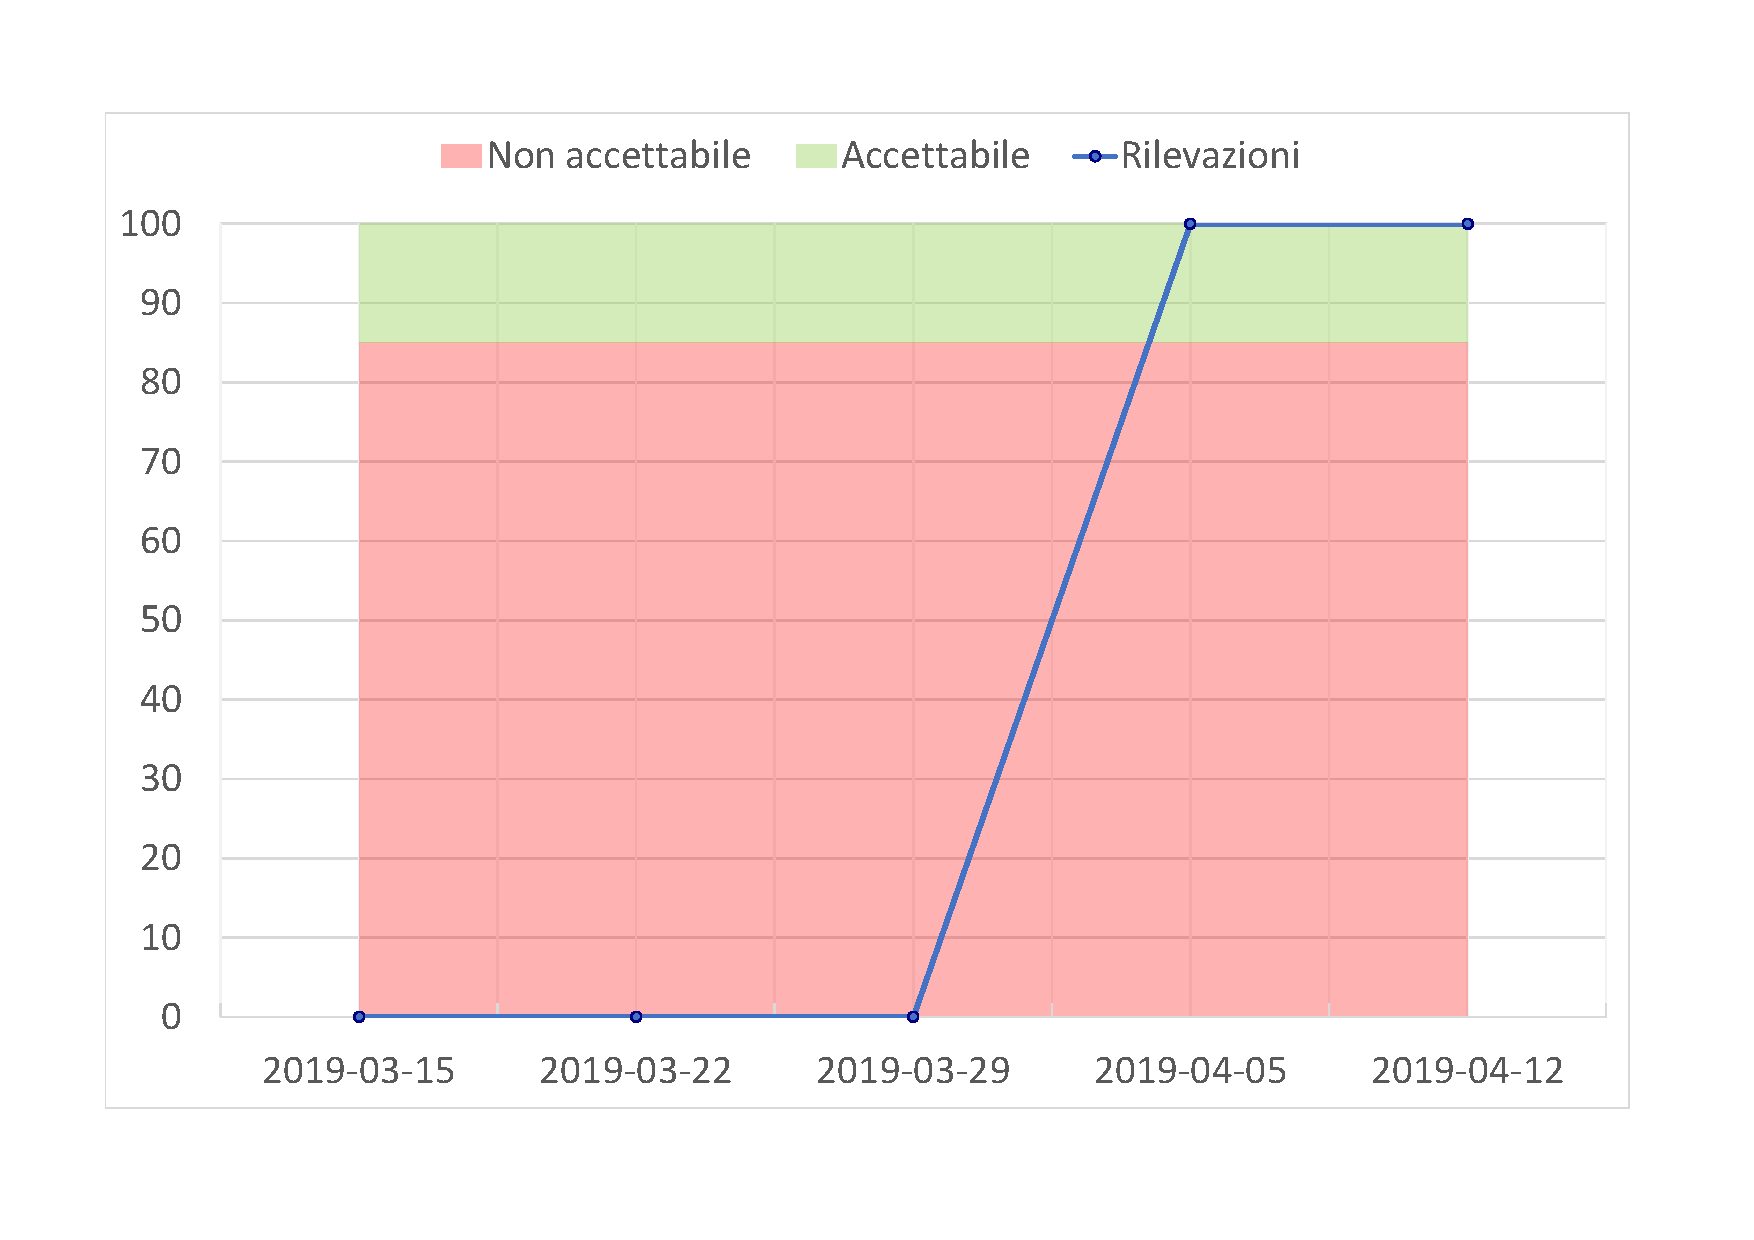
\includegraphics[scale=0.6]{images/resoconto/MPS1Chart.pdf}
	\caption{Serie storica percentuale di superamento test}	
\end{figure}

\paragraph{Numero di parametri per metodo - MPS2}
\subparagraph{Codifica al 2019-04-05}
In questo periodo dell'attività di codifica, la media di parametri per metodo equivale a 1. Infatti sono stati implementati 75 metodi con un totale di 95 parametri.

\subparagraph{Codifica al 2019-04-12}
In questo periodo dell'attività di codifica, la media di parametri per metodo è inferiore a 1. Infatti sono stati implementati 74 metodi con un totale di 44 parametri per un totale di 149 metodi e 139 parametri.

\subparagraph{Codifica al 2019-04-19}
In questo periodo dell'attività di codifica, la media di parametri per metodo è superiore a 1. Infatti sono stati implementati 9 metodi con un totale di 10 parametri per un totale di 158 metodi e 148 parametri.

\subparagraph{Codifica al 2019-04-26}
In questo periodo dell'attività di codifica, la media di parametri per metodo è 1. Infatti sono stati implementati 9 metodi con un totale di 9 parametri per un totale di 167 metodi e 157 parametri.

\subparagraph{Codifica al 2019-05-03}
In questo periodo dell'attività di codifica, la media di parametri per metodo è 0. Infatti sono stati implementati 5 metodi con un totale di 0 parametri per un totale di 172 metodi e 157 parametri. 
A seguito di questa attività di codifica, il prodotto si ritiene concluso all'implementazione.

\subparagraph{Codifica al 2019-05-10}
In questo periodo non si è verificata l'attività di codifica in quanto il prodotto è stato ritenuto concluso precedentemente.
\\
\begin{figure}[H]
	\centering
	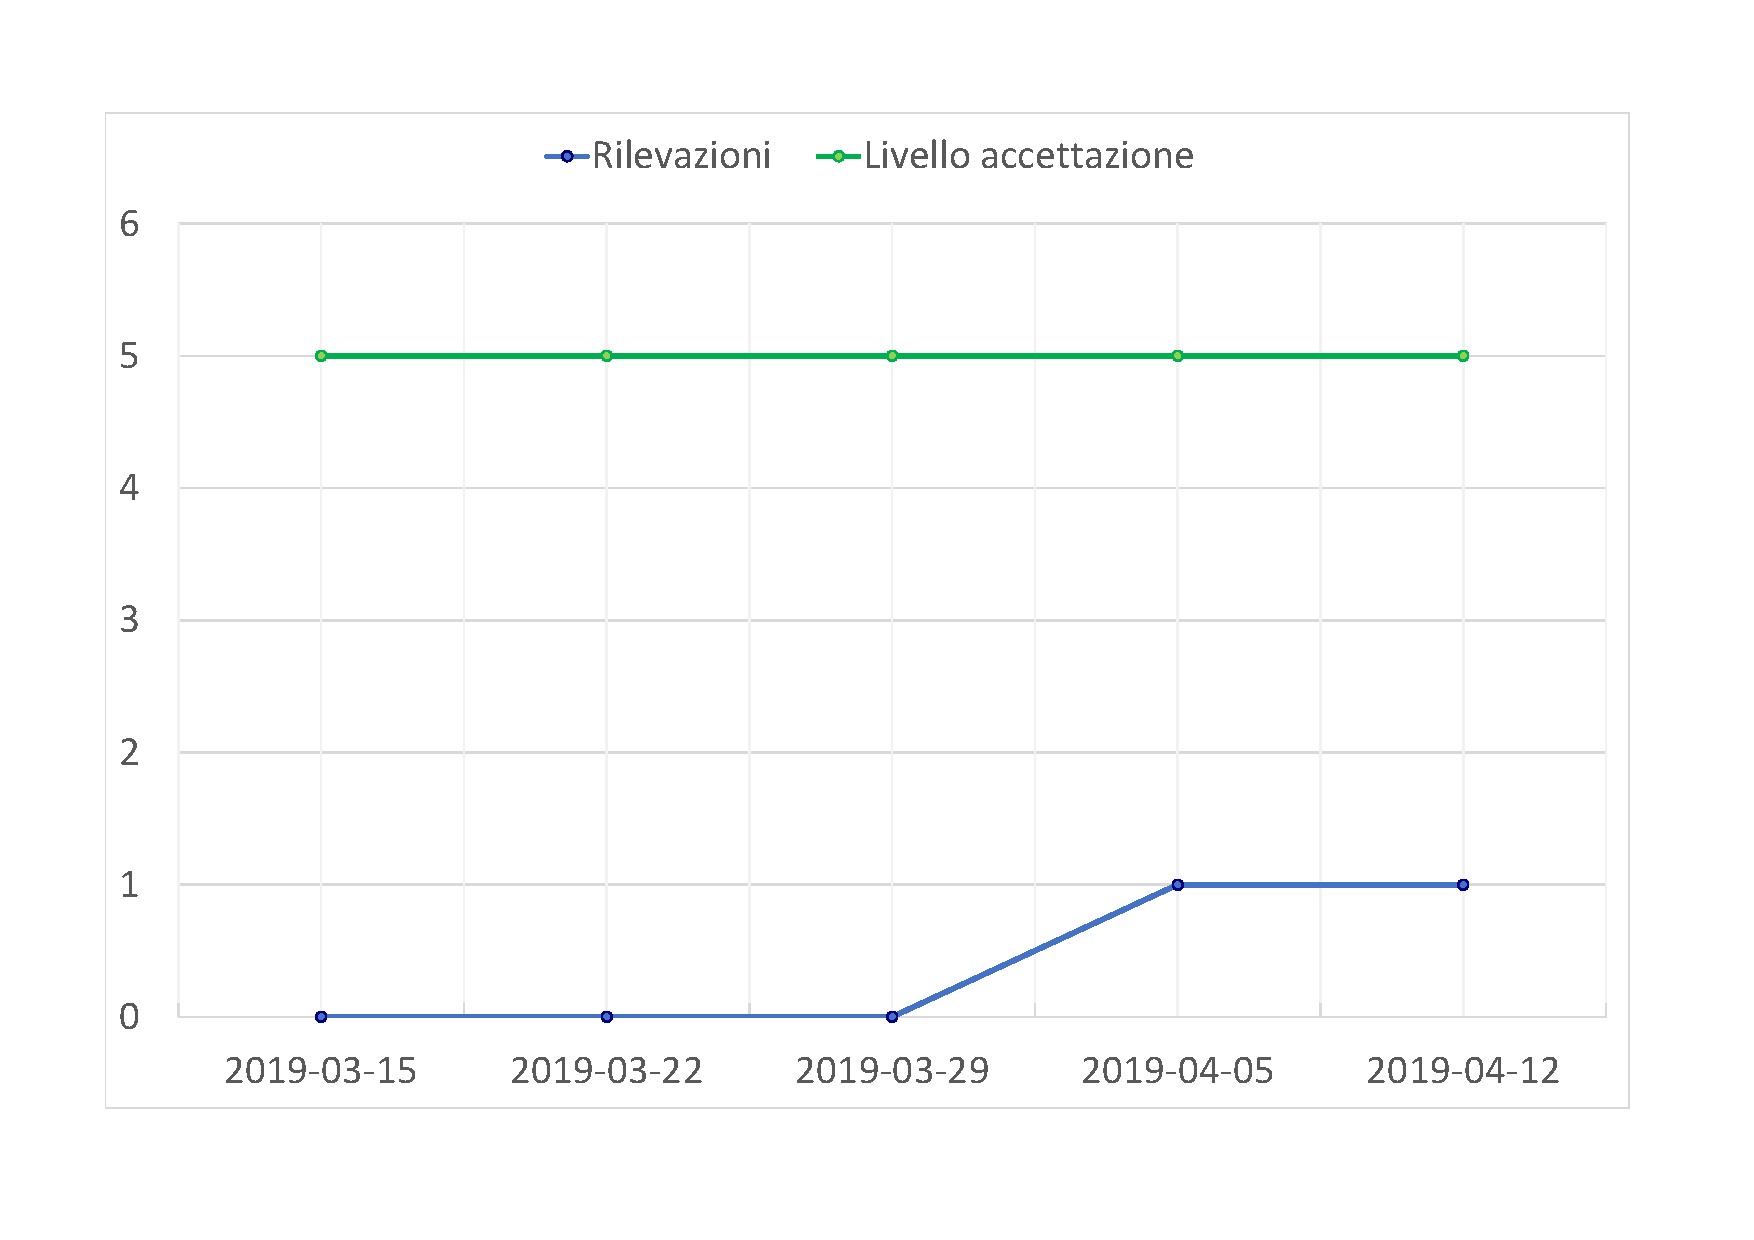
\includegraphics[scale=0.6]{images/resoconto/MPS2Chart.pdf}
	\caption{Serie storica numero di parametri per metodo}	
\end{figure}

\paragraph{Numero di attributi per classe - MPS3}
\subparagraph{Codifica al 2019-04-05}
In questo periodo dell'attività di codifica, la media di attributi per classe equivale a 2. Infatti sono stati implementate 23 classi con un totale di 37 attributi.

\subparagraph{Codifica al 2019-04-12}
In questo periodo dell'attività di codifica, la media di attributi per classe equivale a 1. Infatti sono stati implementate 10 classi con un totale di 7 attributi per un totale di 33 classi e 43 attributi.

\subparagraph{Codifica al 2019-04-19}
In questo periodo dell'attività di codifica, la media di attributi per classe equivale a 0. Infatti non è stata implementata completamente una classe.

\subparagraph{Codifica al 2019-04-26}
In questo periodo dell'attività di codifica, la media di attributi per classe è 3. Infatti è stata implementata 1 classe con 3 attributi per un totale di 34 classi e 46 attributi.

\subparagraph{Codifica al 2019-05-03}
In questo periodo dell'attività di codifica, la media di attributi per classe è 3. Infatti è stata implementata 1 classe con 3 attributi per un totale di 35 classi e 46 attributi.
A seguito di questa attività di codifica, il prodotto si ritiene concluso all'implementazione.

\subparagraph{Codifica al 2019-05-10}
In questo periodo non si è verificata l'attività di codifica in quanto il prodotto è stato ritenuto concluso precedentemente.

\begin{figure}[H]
	\centering
	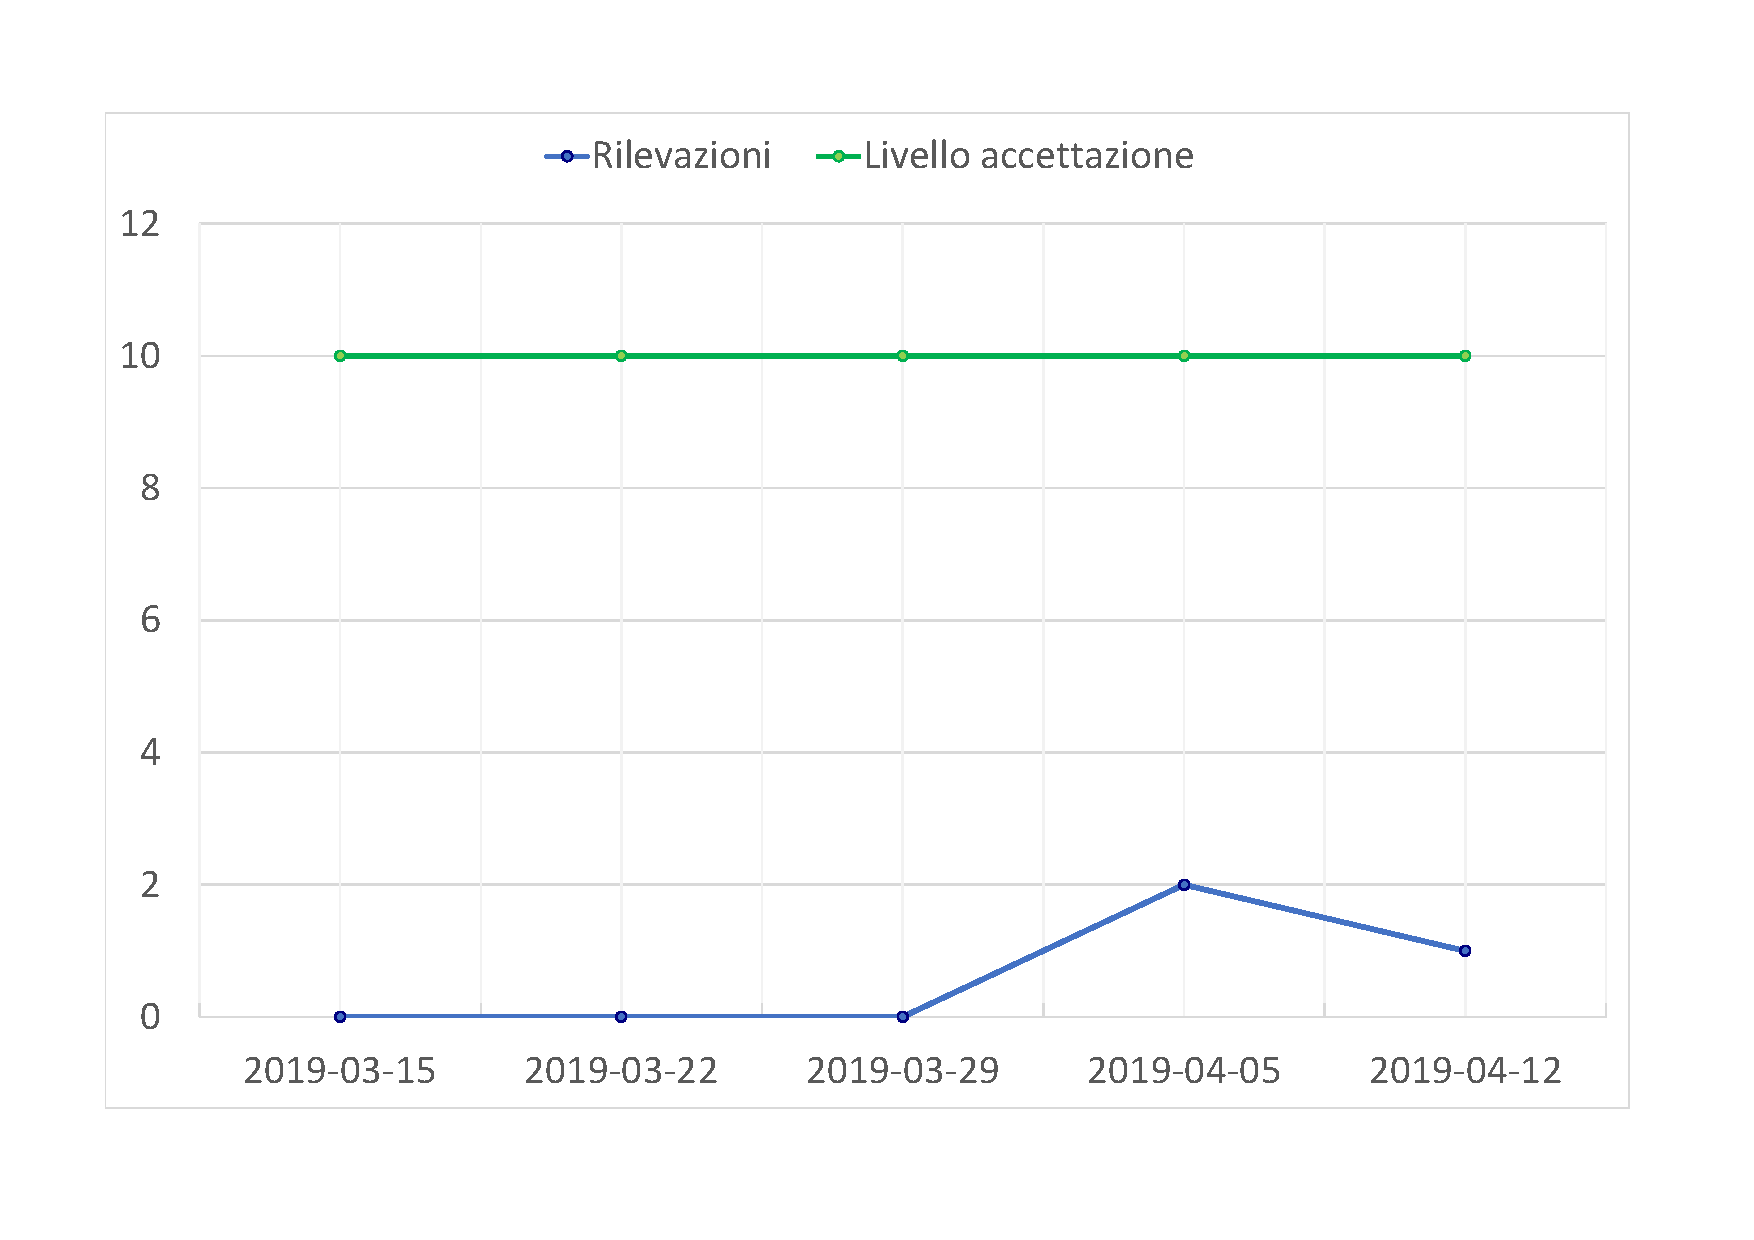
\includegraphics[scale=0.6]{images/resoconto/MPS3Chart.pdf}
	\caption{Serie storica numero di attributi per classe}	
\end{figure}

\paragraph{Numero di metodi per classe - MPS4}
\subparagraph{Codifica al 2019-04-05}
In questo periodo dell'attività di codifica, la media di metodi per classe equivale a 3. Infatti sono stati implementate 23 classi con un totale di 75 metodi.

\subparagraph{Codifica al 2019-04-12}
In questo periodo dell'attività di codifica, la media di metodi per classe equivale a 4.5. Infatti sono state implementate 10 classi con un totale di 74 metodi per un totale di 33 classi e 149 metodi.

\subparagraph{Codifica al 2019-04-19}
In questo periodo dell'attività di codifica, la media di metodi per classe equivale a 0. Infatti non è stata implementata completamente una classe.

\subparagraph{Codifica al 2019-04-26}
In questo periodo dell'attività di codifica, la media di metodi per classe equivale a 18. Infatti è stata implementata 1 classe con un totale di 18 metodi per un totale di 34 classi e 167 metodi.

\subparagraph{Codifica al 2019-05-03}
In questo periodo dell'attività di codifica, la media di metodi per classe equivale a 5. Infatti è stata implementata 1 classe con un totale di 5 metodi per un totale di 35 classi e 172 metodi.

\subparagraph{Codifica al 2019-05-10}
In questo periodo non si è verificata l'attività di codifica in quanto il prodotto è stato ritenuto concluso precedentemente.

\begin{figure}[H]
	\centering
	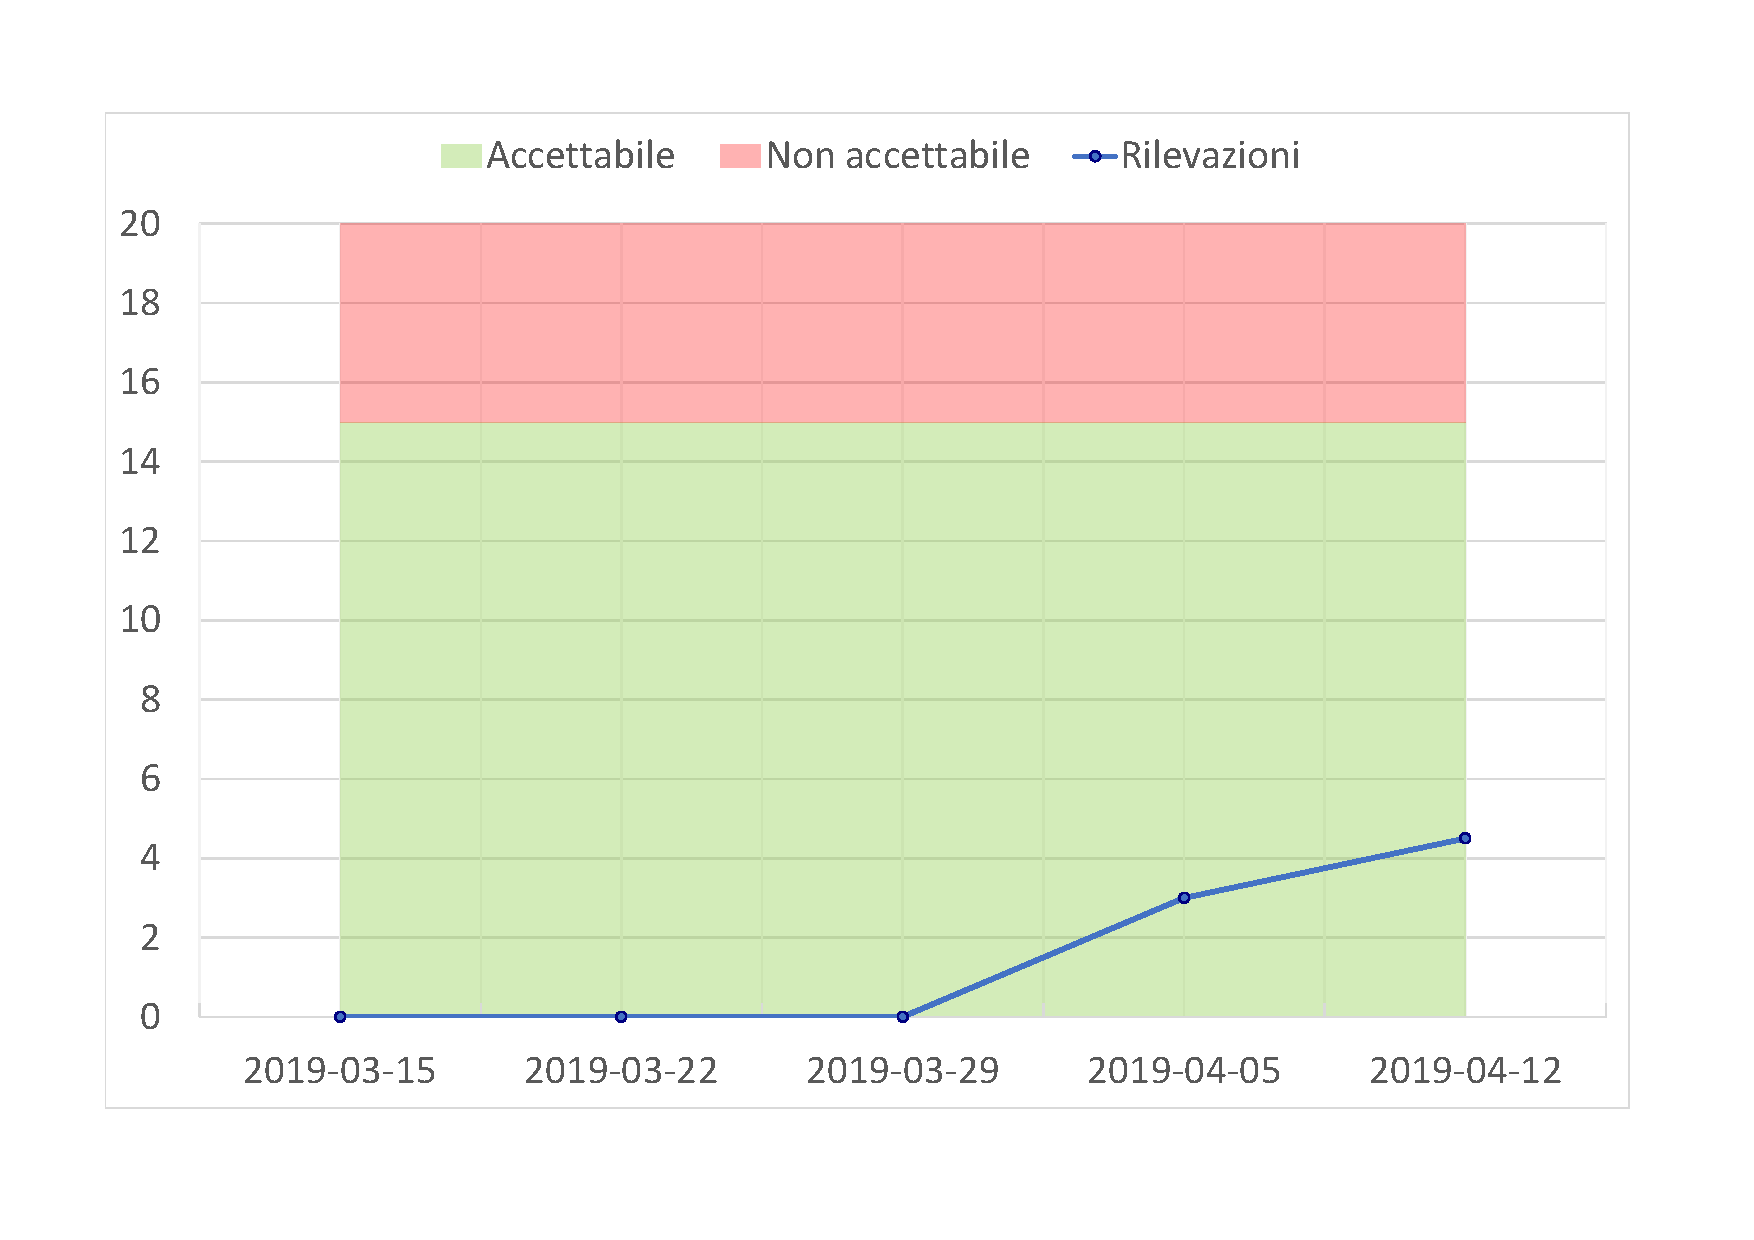
\includegraphics[scale=0.6]{images/resoconto/MPS4Chart.pdf}
	\caption{Serie storica rilevazioni numero di metodi per classe}	
\end{figure}

\paragraph{Complessità ciclomatica media - MPS5}
\subparagraph{Codifica al 2019-04-05}
In questo periodo dell'attività di codifica, la complessità ciclomatica media di 74 metodi sviluppati è di circa 1.61. 

\subparagraph{Codifica al 2019-04-12}
In questo periodo dell'attività di codifica, son stati sviluppati 75 metodi, con un totale di 149 e un indice di complessità ciclomatica media di circa 1.20.

\subparagraph{Codifica al 2019-04-19}
In questo periodo dell'attività di codifica, la complessità ciclomatica media di 149 metodi sviluppati è di circa 1.22. 

\subparagraph{Codifica al 2019-04-26}
In questo periodo dell'attività di codifica, la complessità ciclomatica media di 167 metodi sviluppati è di circa 1.35. 

\subparagraph{Codifica al 2019-05-03}
In questo periodo dell'attività di codifica, la complessità ciclomatica media di 172 metodi sviluppati è di circa 1.28. 

\subparagraph{Codifica al 2019-05-10}
In questo periodo non si è verificata l'attività di codifica in quanto il prodotto è stato ritenuto concluso precedentemente.

\begin{figure}[H]
	\centering
	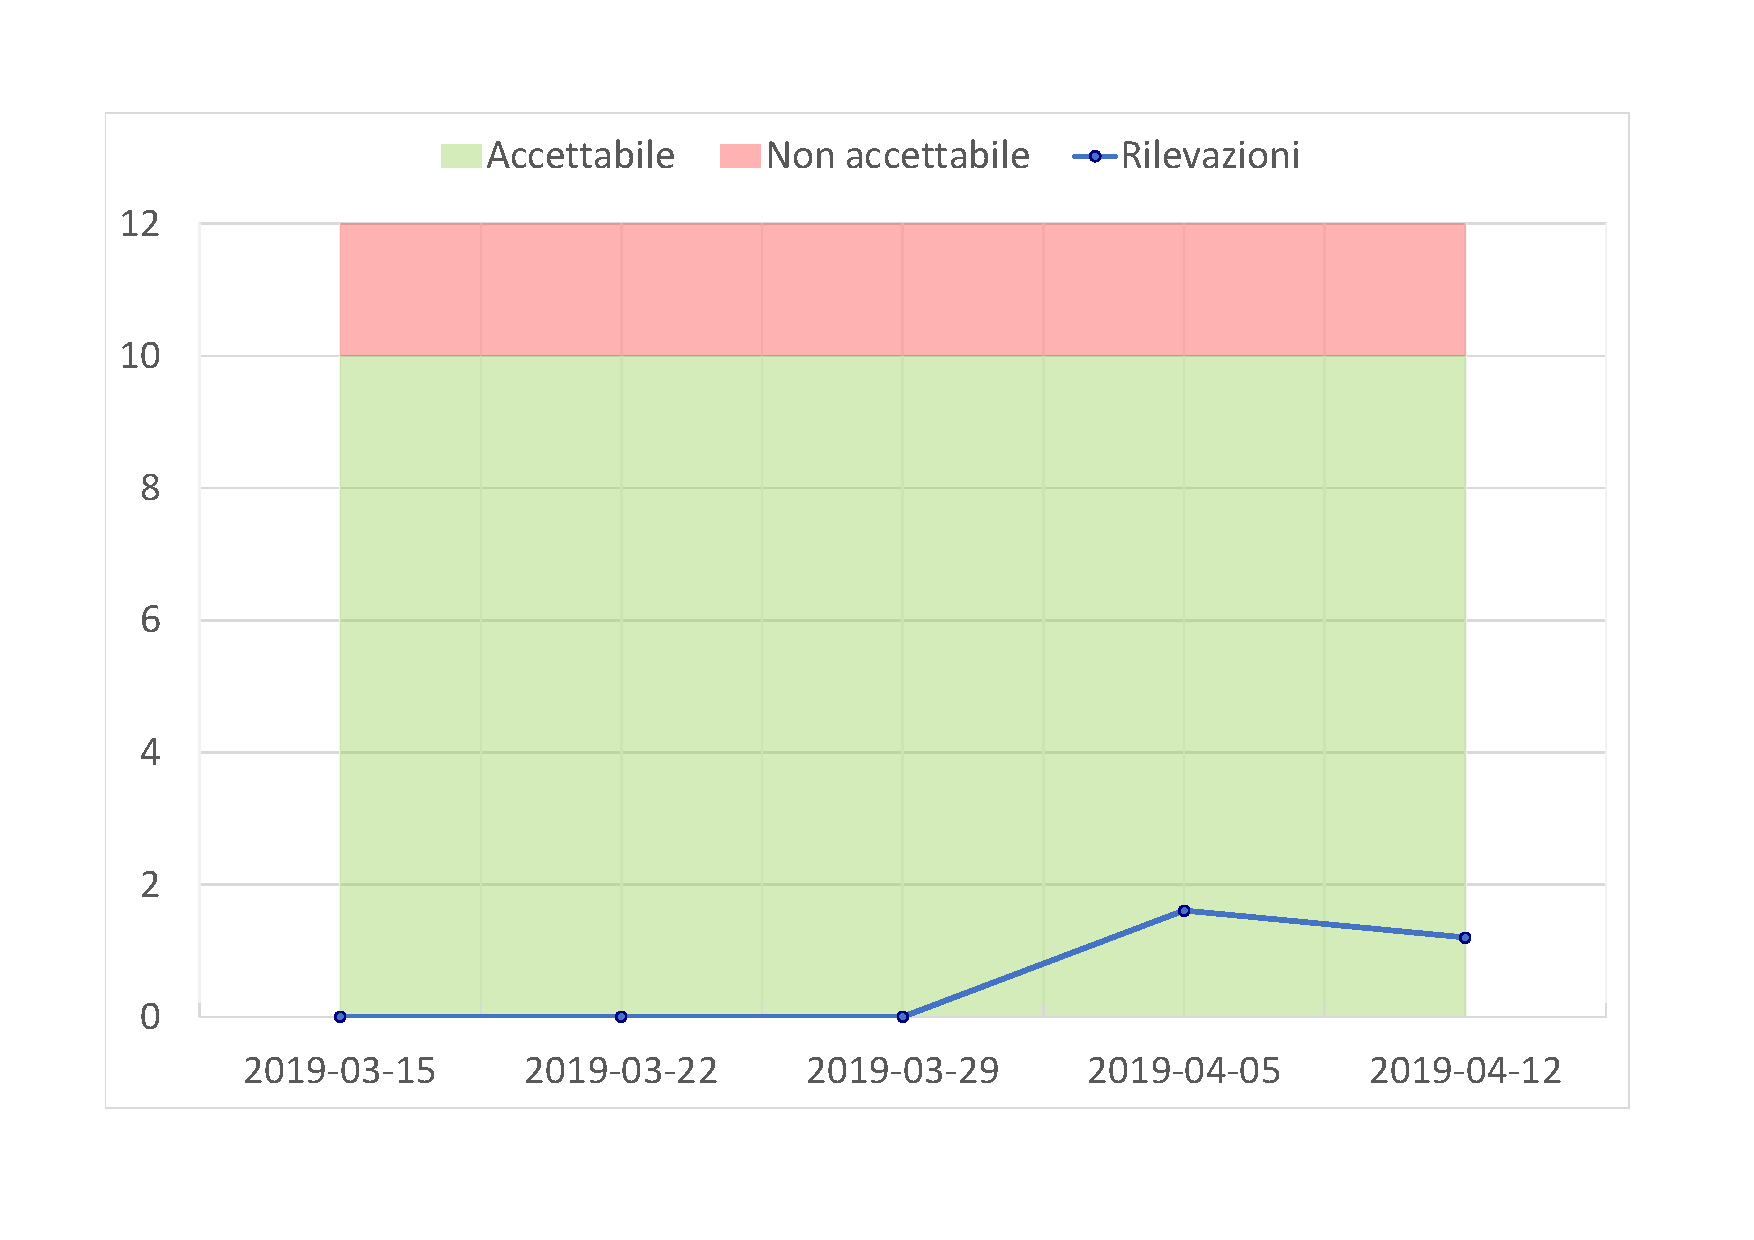
\includegraphics[scale=0.6]{images/resoconto/MPS5Chart.pdf}
	\caption{Serie storica rilevazioni numero di metodi per classe}	
\end{figure}


\paragraph{Implementazione dei requisiti obbligatori - MPS6}
\subparagraph{Codifica al 2019-04-05}
In questo periodo dell'attività di codifica, sono stati soddisfatti 26 requisiti obbligatori, ovvero il 56,52\% dei requisiti obbligatori totali.
Nonostante non raggiunga il livello di accettazione della
metrica, questo risultato è ritenuto sufficiente a questo punto del progetto poiché sono previsti altri incrementi alla codifica che porteranno al soddisfacimento di altri requisiti.

\subparagraph{Codifica al 2019-04-12}
In questo periodo dell'attività di codifica, sono stati soddisfatti 12 requisiti obbligatori, per un totale di 38, ovvero l'82,60\% dei requisiti obbligatori totali.
Nonostante non raggiunga il livello di accettazione della
metrica, questo risultato è ritenuto sufficiente a questo punto del progetto poiché sono previsti altri incrementi alla codifica che porteranno al soddisfacimento di altri requisiti.

\subparagraph{Codifica al 2019-04-19}
In questo periodo dell'attività di codifica, sono stati soddisfatti 12 requisiti obbligatori, per un totale di 40, ovvero l'86.95\% dei requisiti obbligatori totali.
Nonostante non raggiunga il livello di accettazione della
metrica, questo risultato è ritenuto sufficiente a questo punto del progetto poiché sono previsti altri incrementi alla codifica che porteranno al soddisfacimento di altri requisiti.

\subparagraph{Codifica al 2019-04-26}
In questo periodo dell'attività di codifica, sono stati soddisfatti 12 requisiti obbligatori, per un totale di 43, ovvero il 93.48\% dei requisiti obbligatori totali.
Nonostante non raggiunga il livello di accettazione della
metrica, questo risultato è ritenuto sufficiente a questo punto del progetto poiché sono previsti altri incrementi alla codifica che porteranno al soddisfacimento di altri requisiti.

\subparagraph{Codifica al 2019-05-03}
In questo periodo dell'attività di codifica, sono stati soddisfatti 12 requisiti obbligatori, per un totale di 46, ovvero il 100\% dei requisiti obbligatori totali.
A seguito di questo periodo di codifica la soglia di accettabilità della metrica è stata raggiunta.

\subparagraph{Codifica al 2019-05-10}
In questo periodo non si è verificata l'attività di codifica in quanto il prodotto è stato ritenuto concluso precedentemente.

\begin{figure}[H]
	\centering
	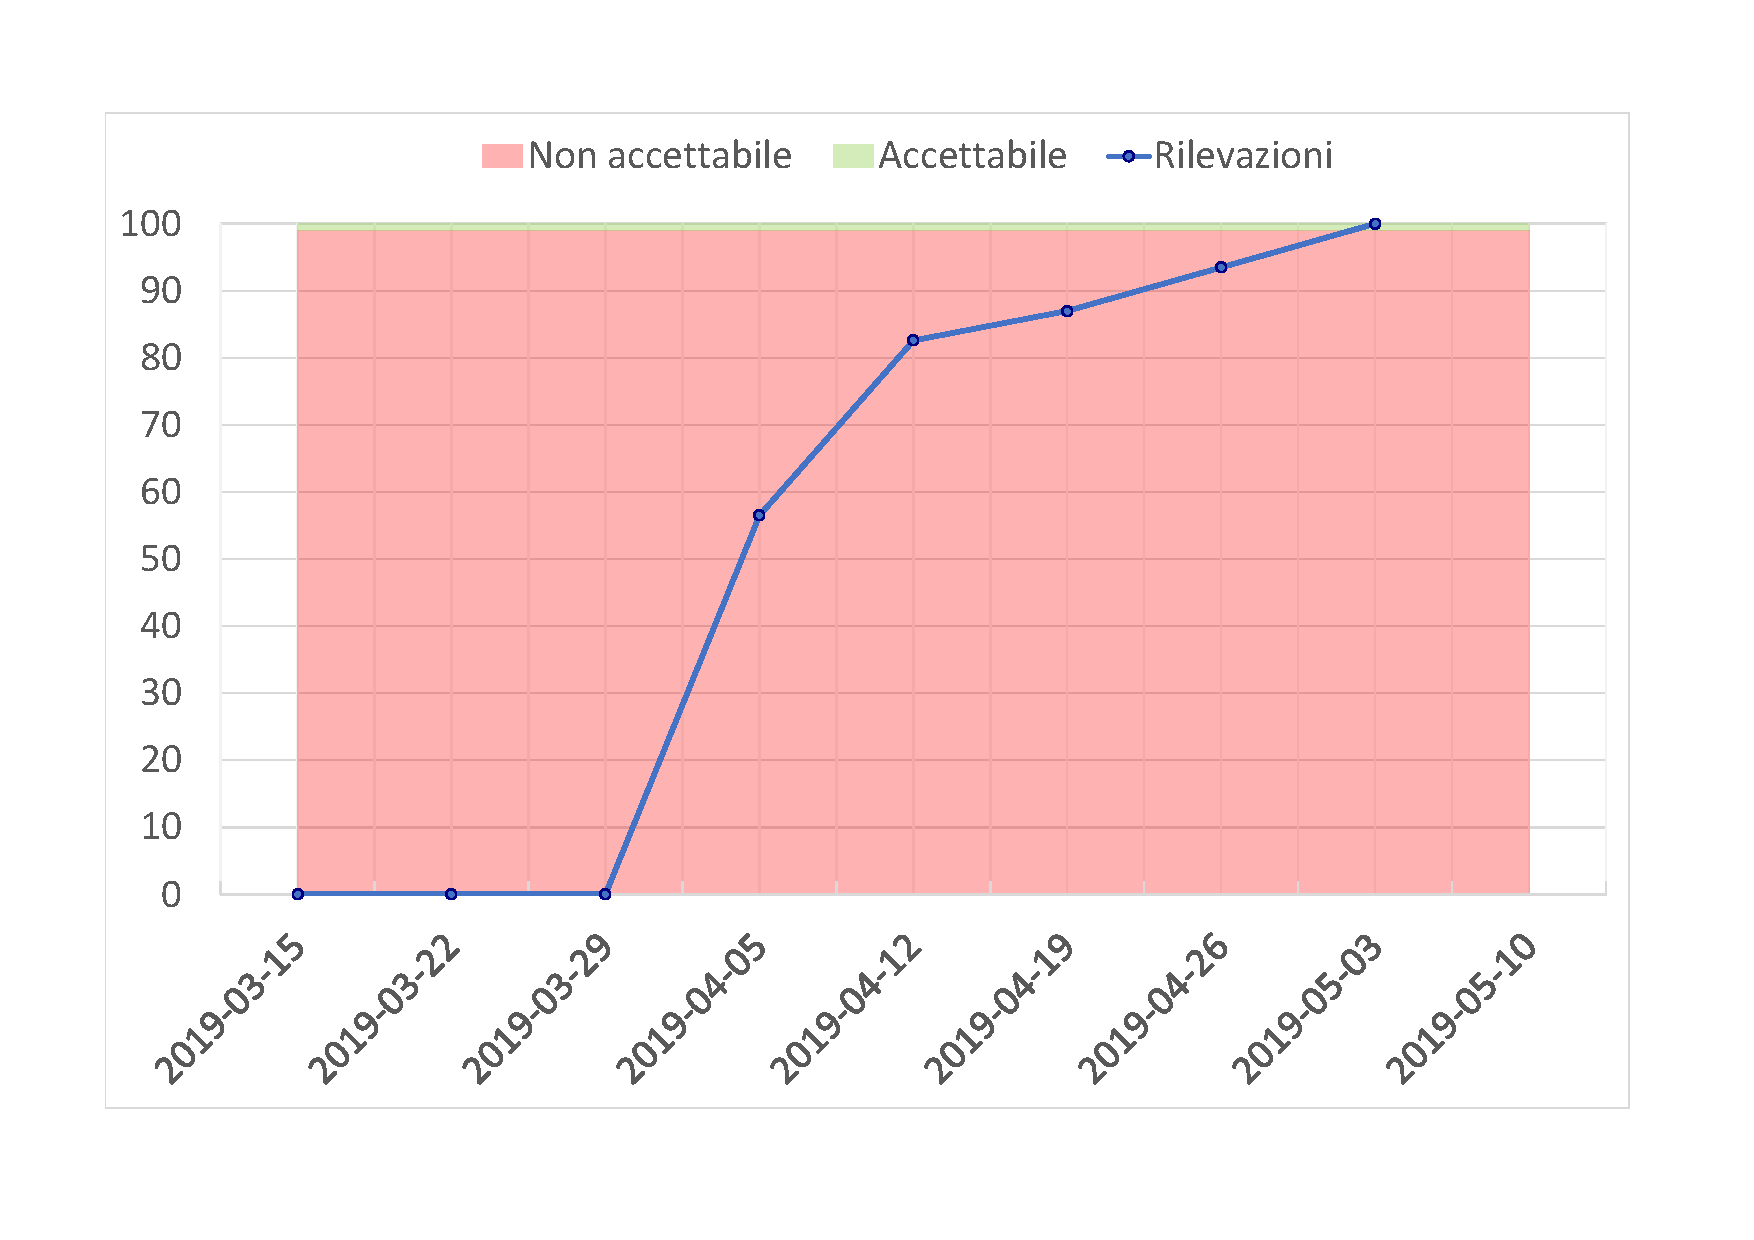
\includegraphics[scale=0.6]{images/resoconto/MPS6Chart.pdf}
	\caption{Serie storica percentuale di requisiti obbligatori soddisfatti}	
\end{figure}

\paragraph{Implementazione dei requisiti desiderabili - MPS7}
\subparagraph{Codifica al 2019-04-05}
In questo periodo dell'attività di codifica, sono stati soddisfatti 6 requisiti desiderabili, ovvero il 13,63\% dei requisiti desiderabili totali.
Nonostante non raggiunga il livello di accettazione della
metrica, questo risultato è ritenuto sufficiente a questo punto del progetto poiché sono previsti altri incrementi alla codifica che porteranno al soddisfacimento di altri requisiti.

\subparagraph{Codifica al 2019-04-12}
In questo periodo dell'attività di codifica, sono stati soddisfatti 4 requisiti desiderabili, per un totale di 10, ovvero il 22,72\% dei requisiti desiderabili totali.
Nonostante non raggiunga il livello di accettazione della
metrica, questo risultato è ritenuto sufficiente a questo punto del progetto poiché sono previsti altri incrementi alla codifica che porteranno al soddisfacimento di altri requisiti.

\subparagraph{Codifica al 2019-04-19}
In questo periodo dell'attività di codifica, sono stati soddisfatti 5 requisiti desiderabili, per un totale di 15, ovvero il 30,61\% dei requisiti desiderabili totali.
A seguito di questo periodo di codifica la soglia di accettabilità della metrica è stata raggiunta.
Il gruppo si impegnerà ad incrementare ulteriormente la copertura di altri requisiti desiderabili.

\subparagraph{Codifica al 2019-04-26}
In questo periodo dell'attività di codifica, sono stati soddisfatti 4 requisiti desiderabili, per un totale di 19, ovvero il 38,77\% dei requisiti desiderabili totali.

\subparagraph{Codifica al 2019-05-03}
In questo periodo dell'attività di codifica, sono stati soddisfatti 6 requisiti desiderabili, per un totale di 25, ovvero il 51,02\% dei requisiti desiderabili totali.

\subparagraph{Codifica al 2019-05-10}
In questo periodo non si è verificata l'attività di codifica in quanto il prodotto è stato ritenuto concluso precedentemente.

\begin{figure}[H]
	\centering
	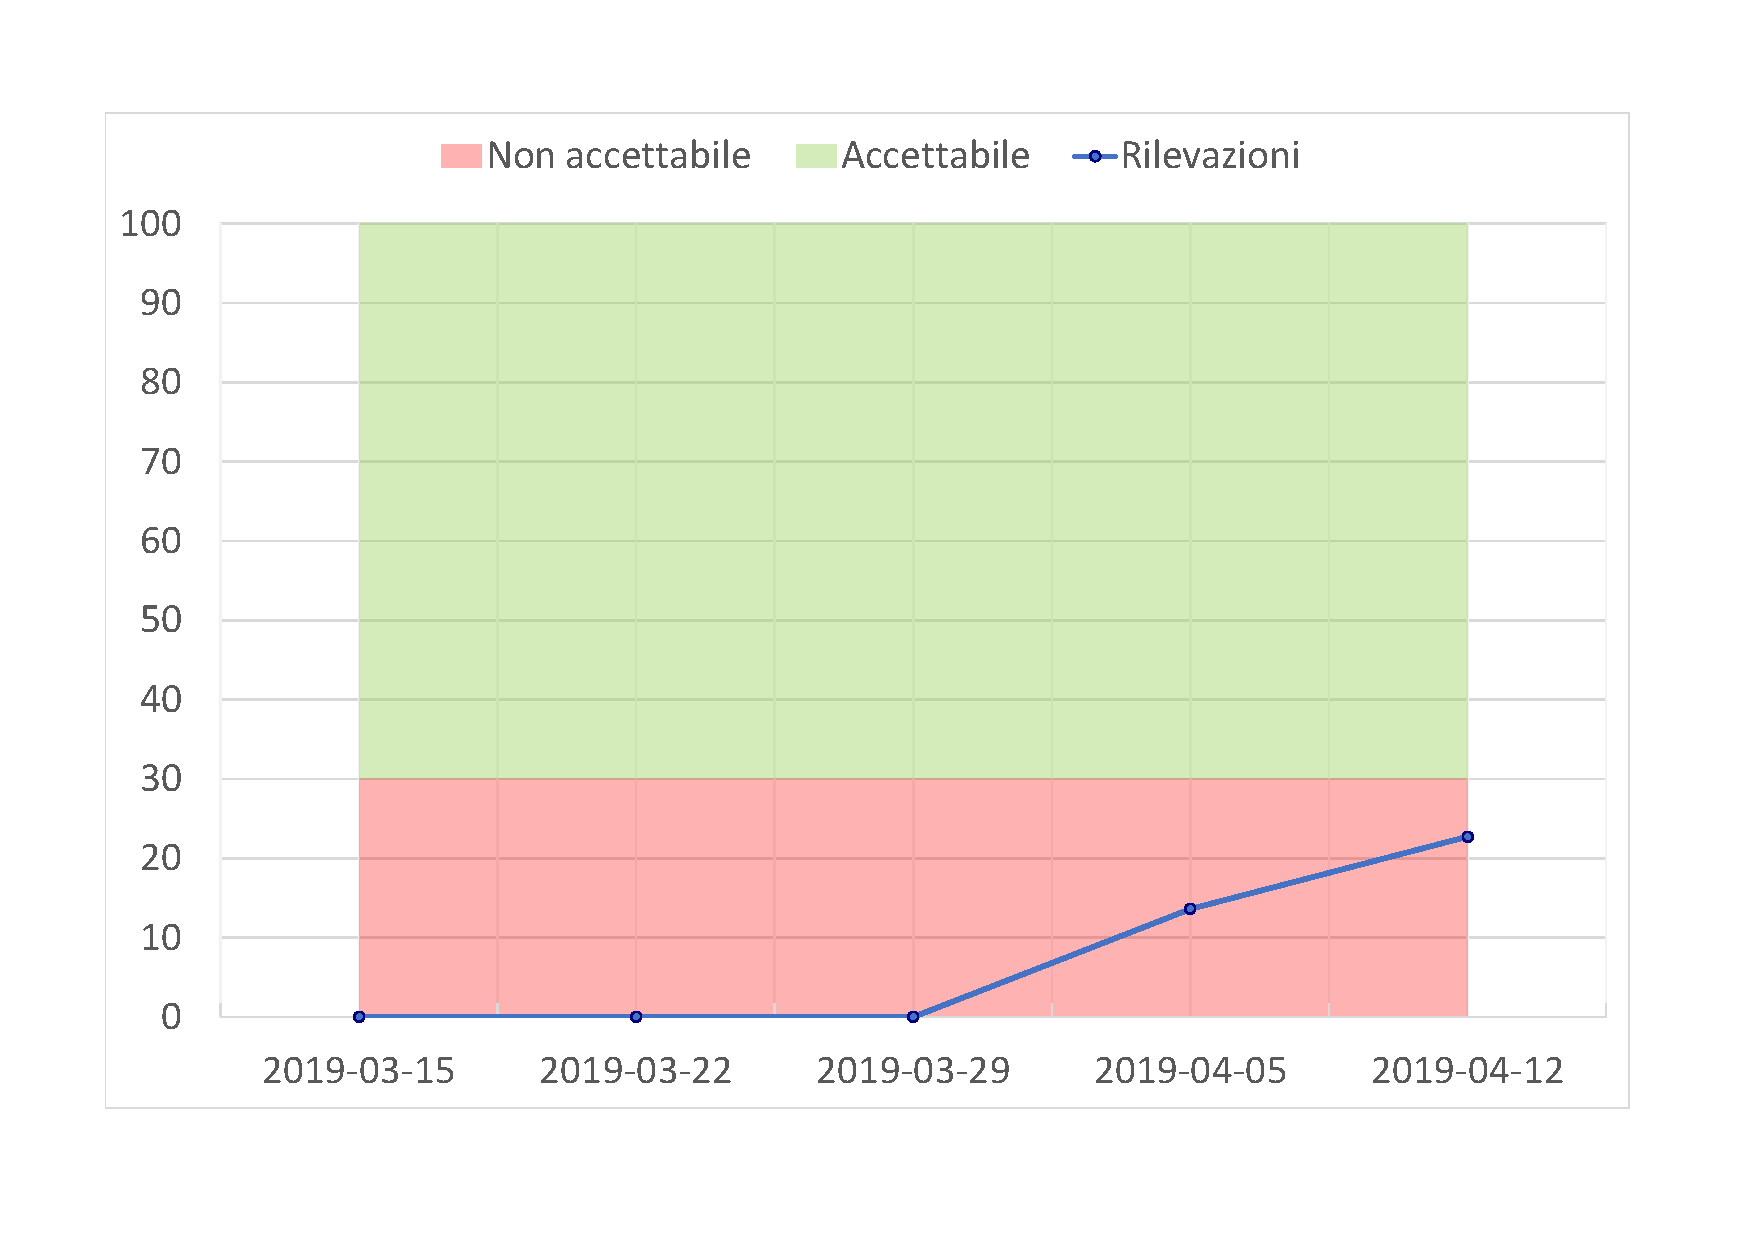
\includegraphics[scale=0.6]{images/resoconto/MPS7Chart.pdf}
	\caption{Serie storica percentuale di requisiti desiderabili soddisfatti}	
\end{figure}

\paragraph{Copertura dei test sul codice - MPS8}
\subparagraph{Codifica al 2019-04-05}
In questo periodo dell'attività di codifica, sono stati implementati 21 test, coprendo circa il 92.47\% degli statements delle classi testate.

\subparagraph{Codifica al 2019-04-12}
In questo periodo dell'attività di codifica, sono stati implementati 21 test, con un totale di 42 test coprendo circa il 89.98\% degli statements delle classi testate.

\subparagraph{Codifica al 2019-04-19}

\subparagraph{Codifica al 2019-04-26}

\subparagraph{Codifica al 2019-05-03}

\subparagraph{Codifica al 2019-05-10}

\begin{figure}[H]
	\centering
	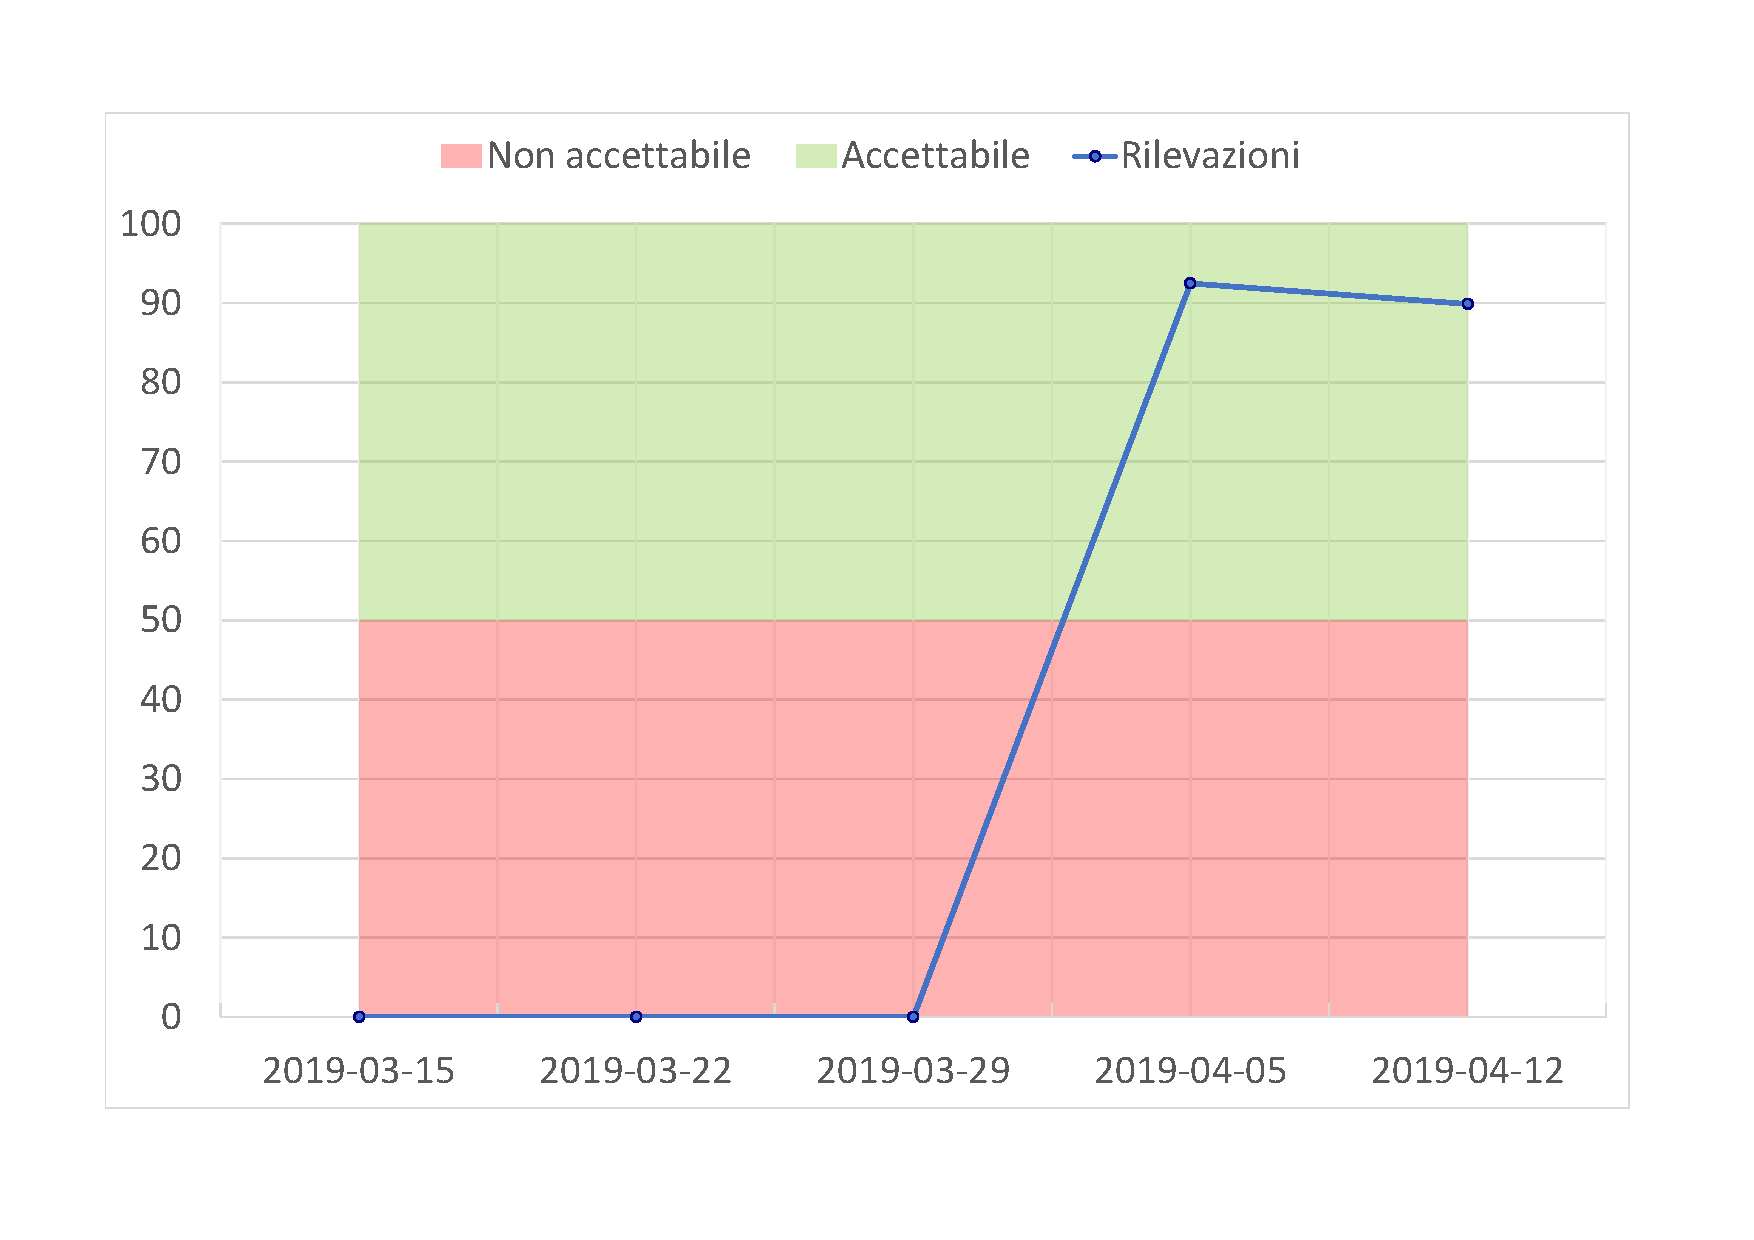
\includegraphics[scale=0.6]{images/resoconto/MPS8Chart.pdf}
	\caption{Serie storica rilevazioni copertura dei test sul codice}	
\end{figure}


\paragraph{Implementazione dei requisiti opzionali - MPS9}
\subparagraph{Codifica al 2019-04-05}
In questo periodo dell'attività di codifica, sono stati soddisfatti 0 requisiti opzionali. Il valore della metrica rimane a 0.

\subparagraph{Codifica al 2019-04-12}
In questo periodo dell'attività di codifica, sono stati soddisfatti 2 requisiti opzionali, ovvero il 6,25\% dei requisiti opzionali totali.
Nonostante non raggiunga il livello di accettazione della
metrica, questo risultato è ritenuto sufficiente a questo punto del progetto poiché sono previsti altri incrementi alla codifica che porteranno al soddisfacimento di altri requisiti.

\subparagraph{Codifica al 2019-04-19}
In questo periodo dell'attività di codifica, sono stati soddisfatti 2 requisiti opzionali, con un totale di 4 requisiti totali implementati, ovvero il 12.50\% dei requisiti opzionali totali.
A seguito di questo periodo di codifica la soglia di accettabilità della metrica è stata raggiunta.
Il gruppo si impegnerà ad incrementare ulteriormente la copertura di altri requisiti opzionali.

\subparagraph{Codifica al 2019-04-26}
In questo periodo dell'attività di codifica, sono stato soddisfatto 1 requisito opzionale, con un totale di 5 requisiti totali implementati, ovvero il 15.63\% dei requisiti opzionali totali.

\subparagraph{Codifica al 2019-05-03}
In questo periodo dell'attività di codifica, sono stato soddisfatto 1 requisito opzionale, con un totale di 6 requisiti totali implementati, ovvero il 18.75\% dei requisiti opzionali totali.

\subparagraph{Codifica al 2019-05-10}
In questo periodo non si è verificata l'attività di codifica in quanto il prodotto è stato ritenuto concluso precedentemente.

\begin{figure}[H]
	\centering
	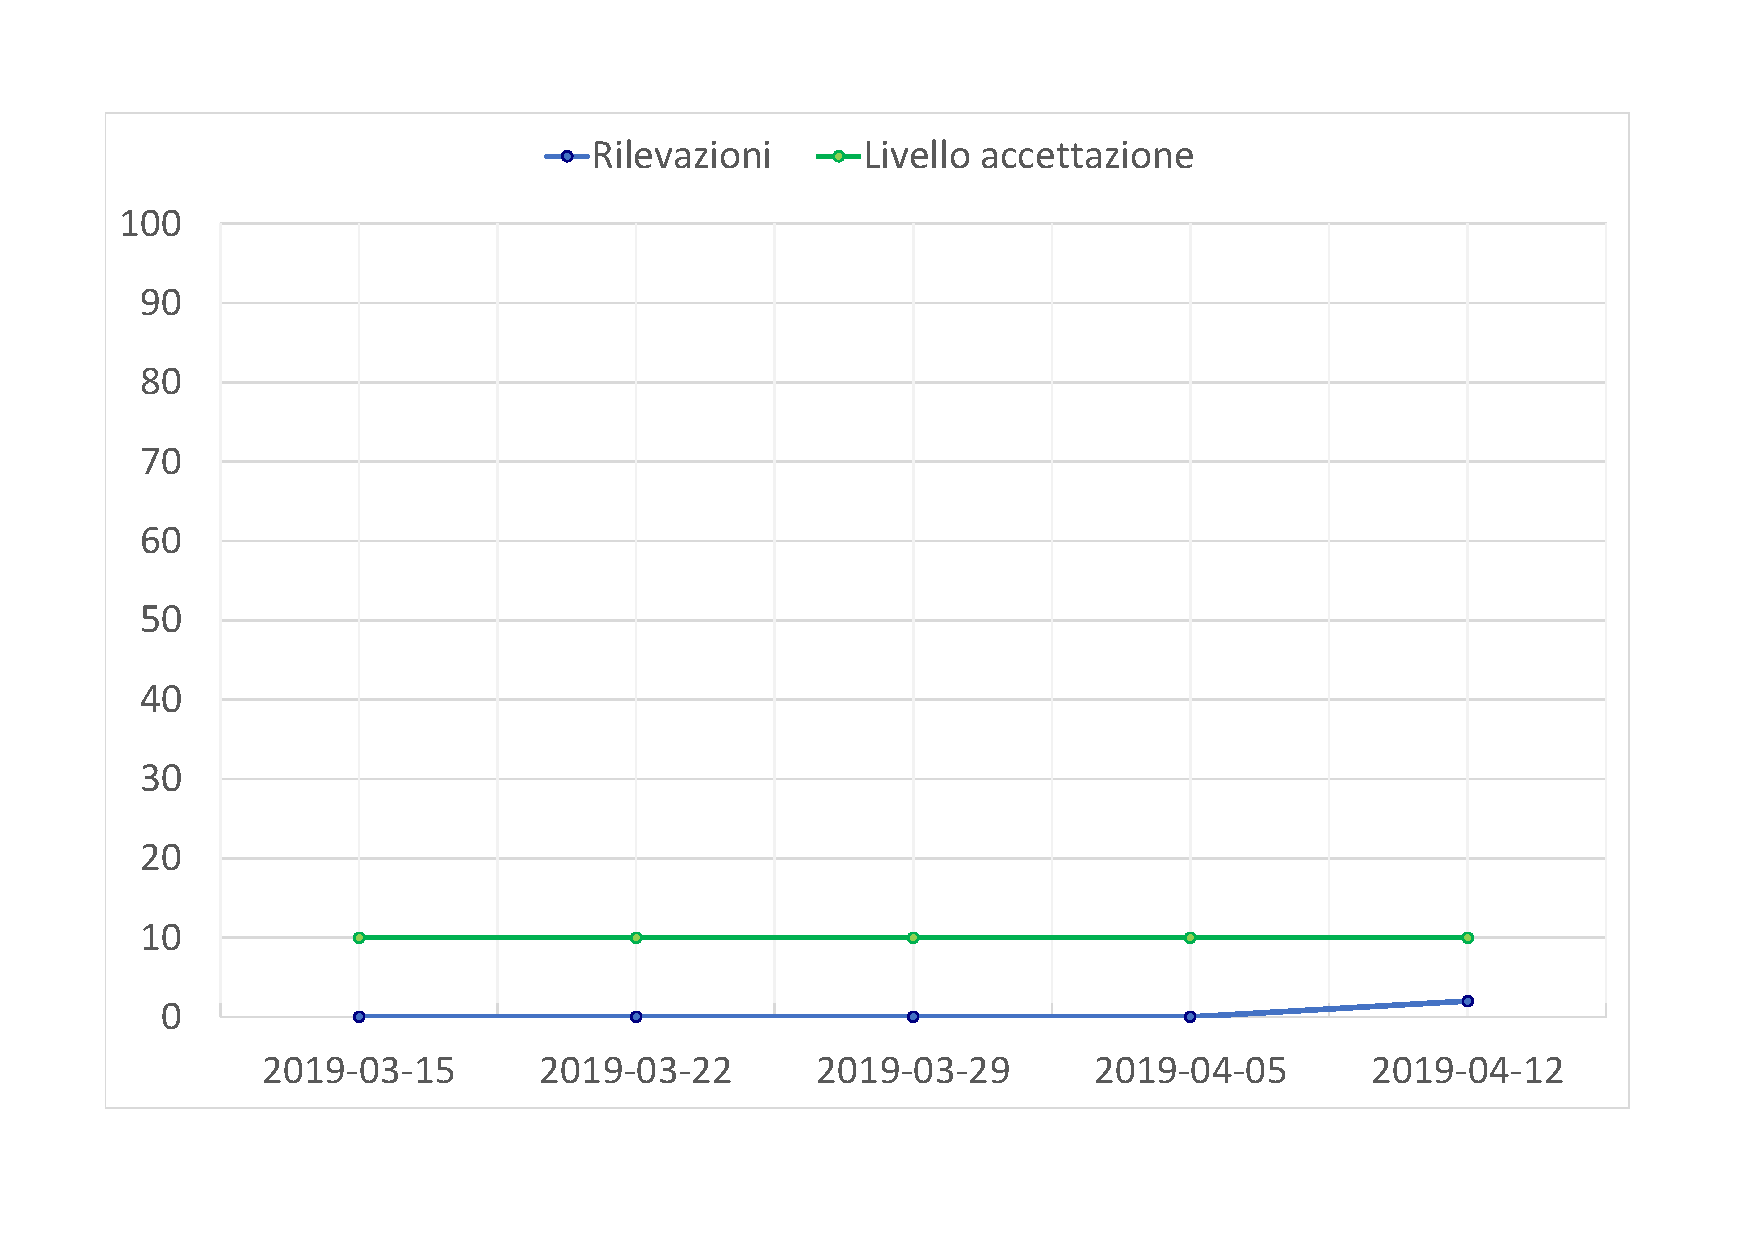
\includegraphics[scale=0.6]{images/resoconto/MPS9Chart.pdf}
	\caption{Serie storica percentuale di requisiti opzionali soddisfatti}	
\end{figure}

\paragraph{Numero di linee di codice di una procedura - MPS10}
\subparagraph{Codifica al 2019-04-05}
In questo periodo dell'attività di codifica, la media di linee di codice per procedura equivale a 20. Infatti sono stati implementati 75 metodi con un totale di circa 1500 linee di codice.

\subparagraph{Codifica al 2019-04-12}
In questo periodo dell'attività di codifica, la media di linee di codice per procedura equivale a 16.77. Infatti sono stati implementati 74 metodi con un totale di circa 1000 linee di codice, per un totale di 149 metodi e 2500 linee di codice.

\subparagraph{Codifica al 2019-04-19}
In questo periodo dell'attività di codifica, la media di linee di codice per procedura equivale a 16.50. Infatti sono stati implementati 9 metodi con un totale di circa 130 linee di codice, per un totale di 158 metodi e 2630 linee di codice.

\subparagraph{Codifica al 2019-04-26}
In questo periodo dell'attività di codifica, la media di linee di codice per procedura equivale a 16.35. Infatti sono stati implementati 9 metodi con un totale di circa 100 linee di codice, per un totale di 167 metodi e 2730 linee di codice.

\subparagraph{Codifica al 2019-05-03}
In questo periodo dell'attività di codifica, la media di linee di codice per procedura equivale a 16.31. Infatti sono stati implementati 5 metodi con un totale di circa 75 linee di codice, per un totale di 172 metodi e 2805 linee di codice.

\subparagraph{Codifica al 2019-05-10}
In questo periodo non si è verificata l'attività di codifica in quanto il prodotto è stato ritenuto concluso precedentemente.

\begin{figure}[H]
	\centering
	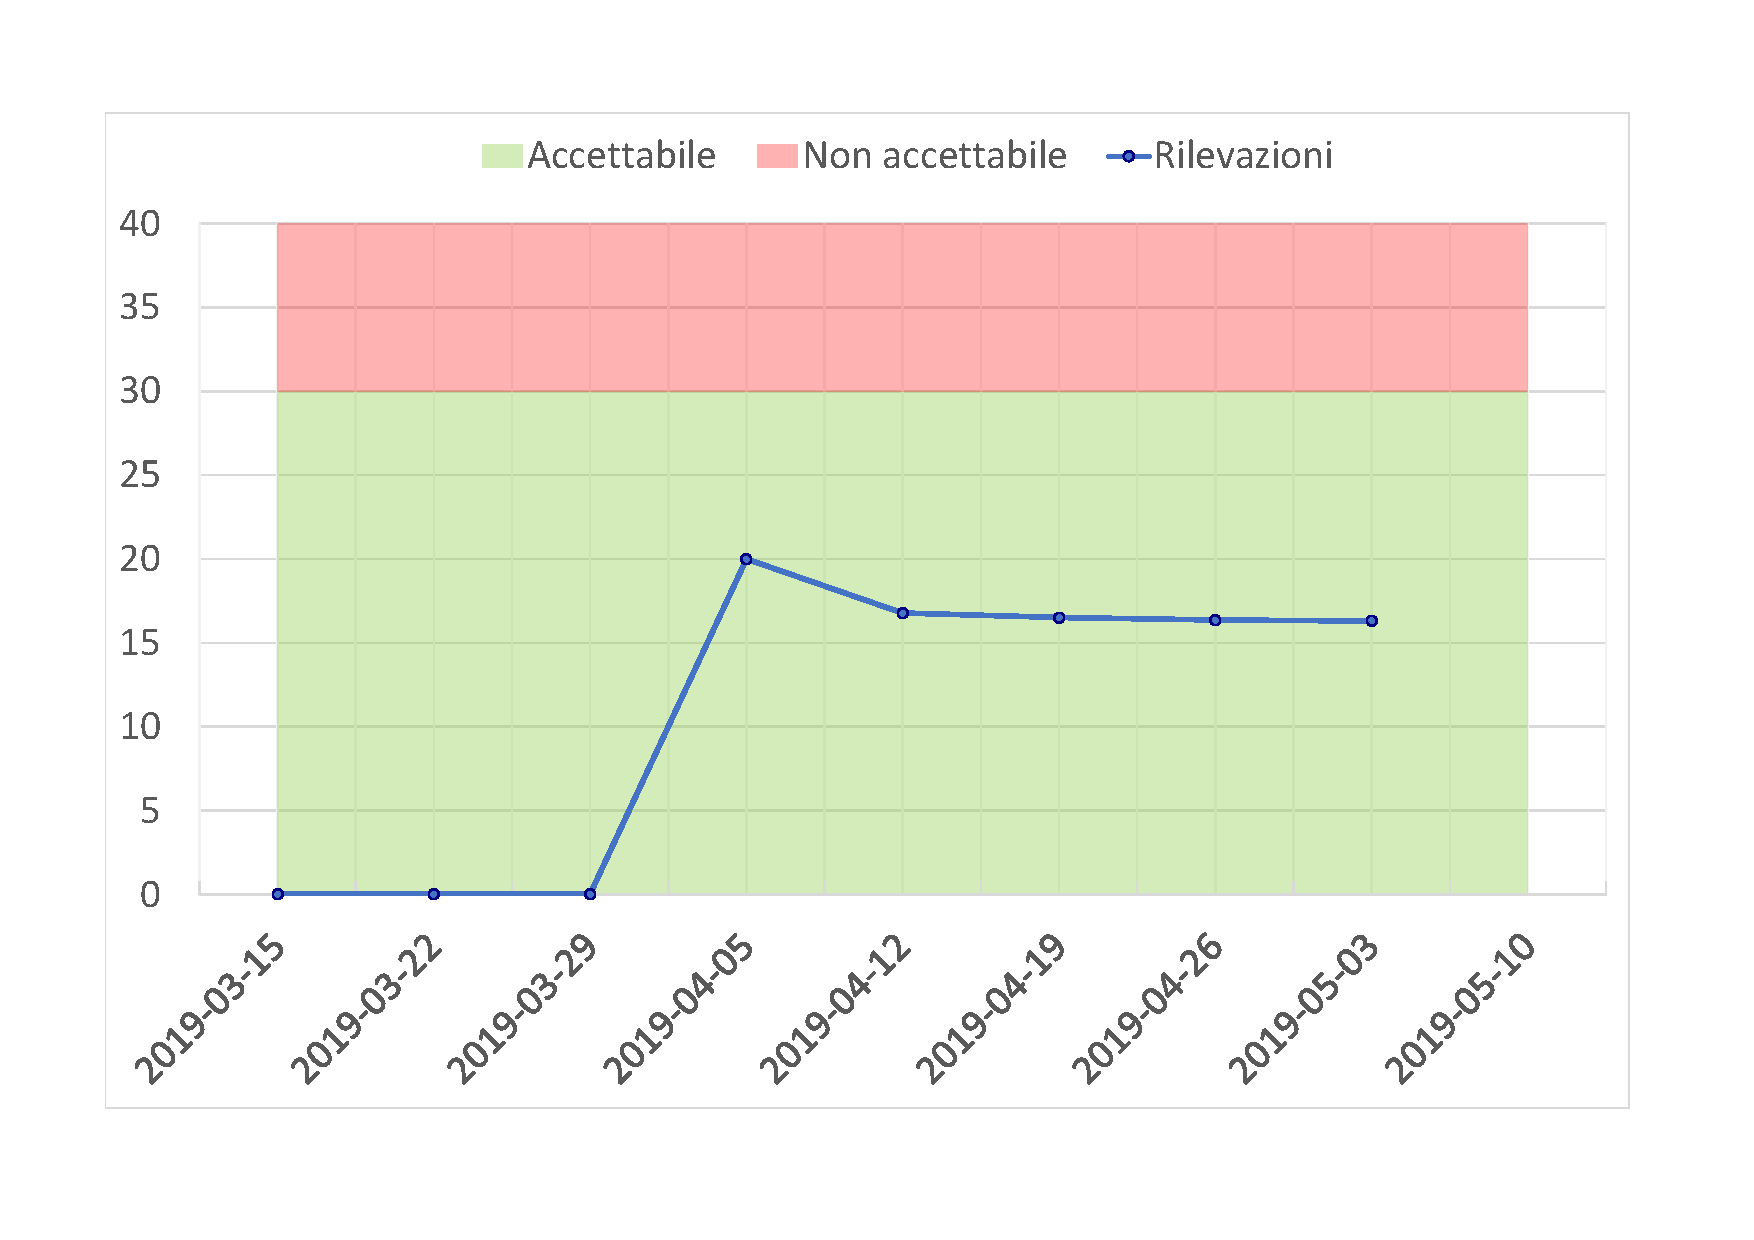
\includegraphics[scale=0.6]{images/resoconto/MPS10Chart.pdf}
	\caption{Serie storica linee di codice per procedura}	
\end{figure}

\subsection{Processi}
\subsubsection{Valori ISO/IEC 15504 - MPC1}

Riportiamo di seguito i grafici rappresentanti il livello raggiunto alla data di ogni revisione dai vari processi.


\begin{figure}[H]
	\centering
	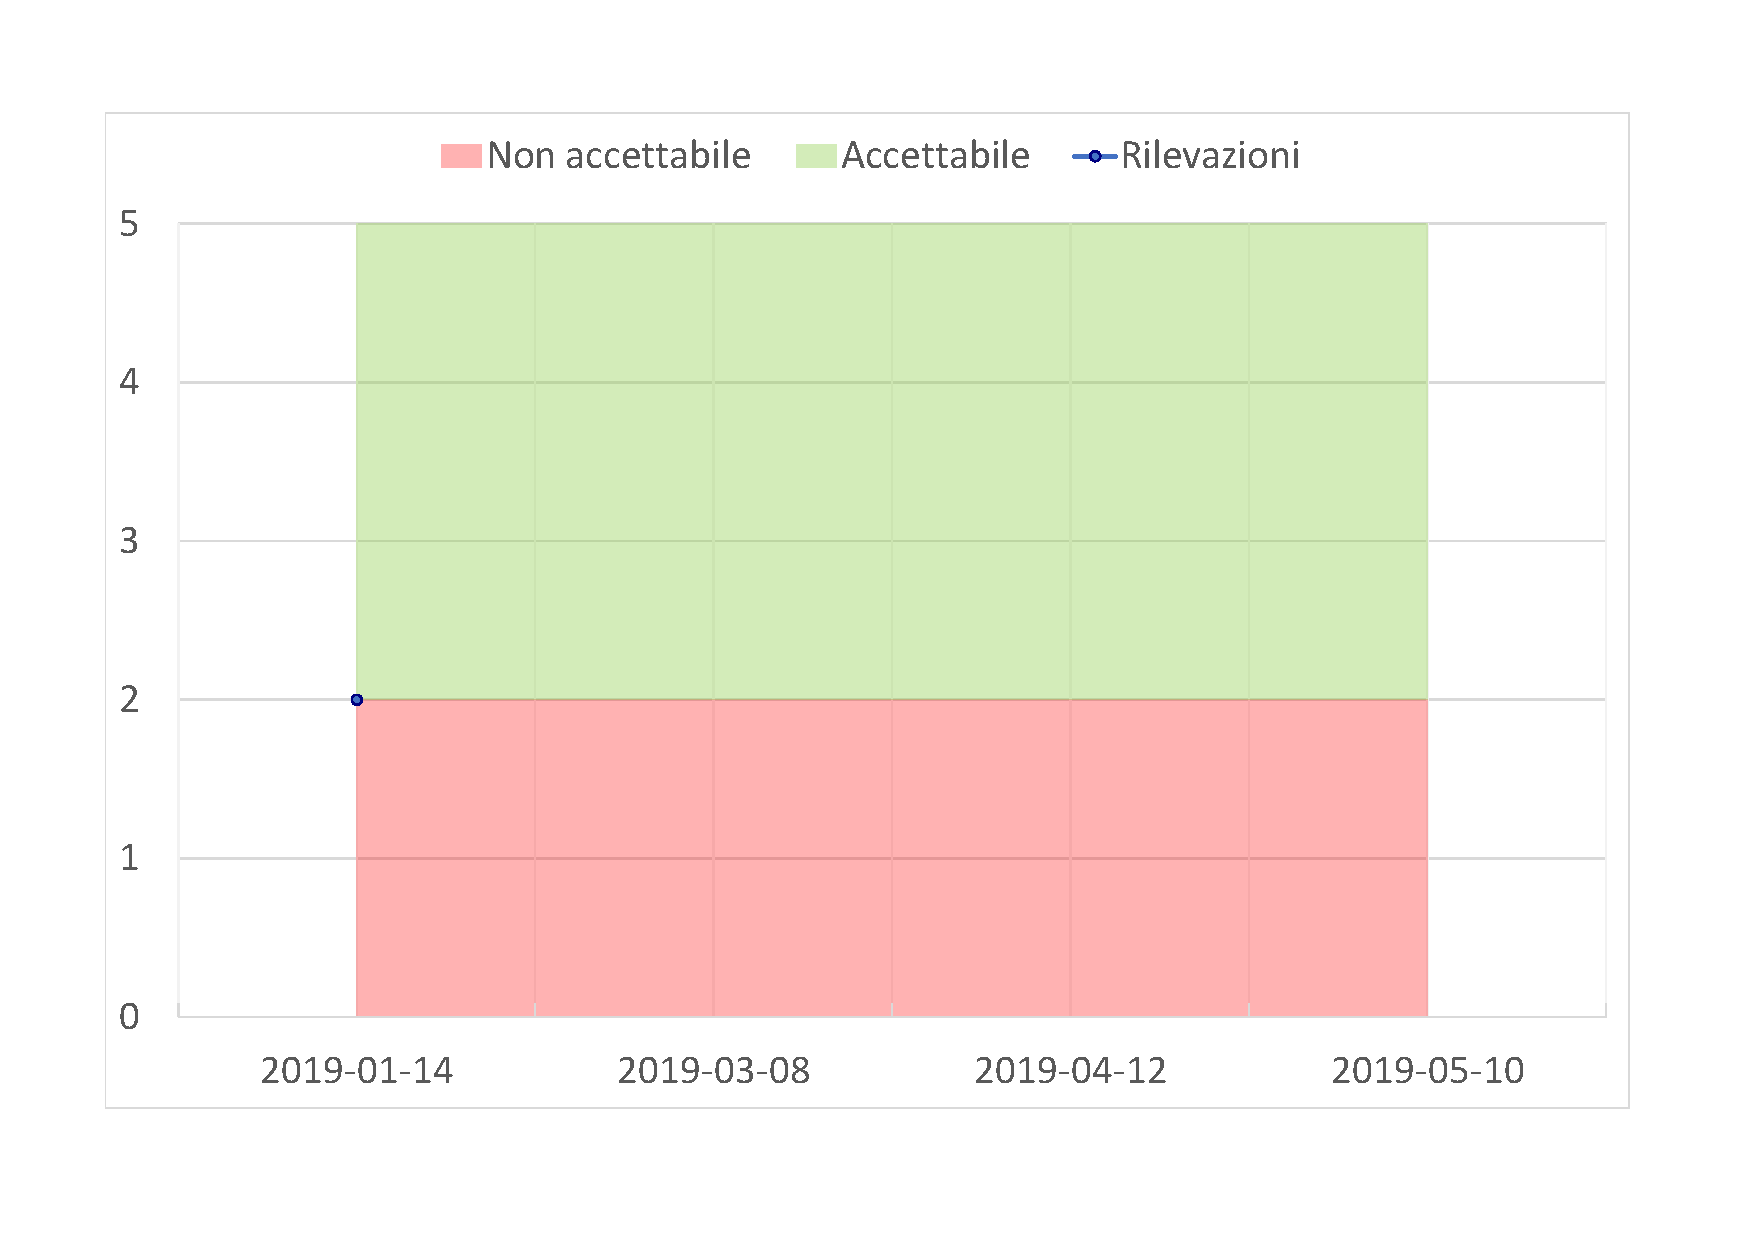
\includegraphics[scale=0.6]{images/resoconto/Studio.pdf}
	\caption{Valori ISO/IEC 15504 - Studio di fattibilità}	
\end{figure}


\begin{figure}[H]
	\centering
	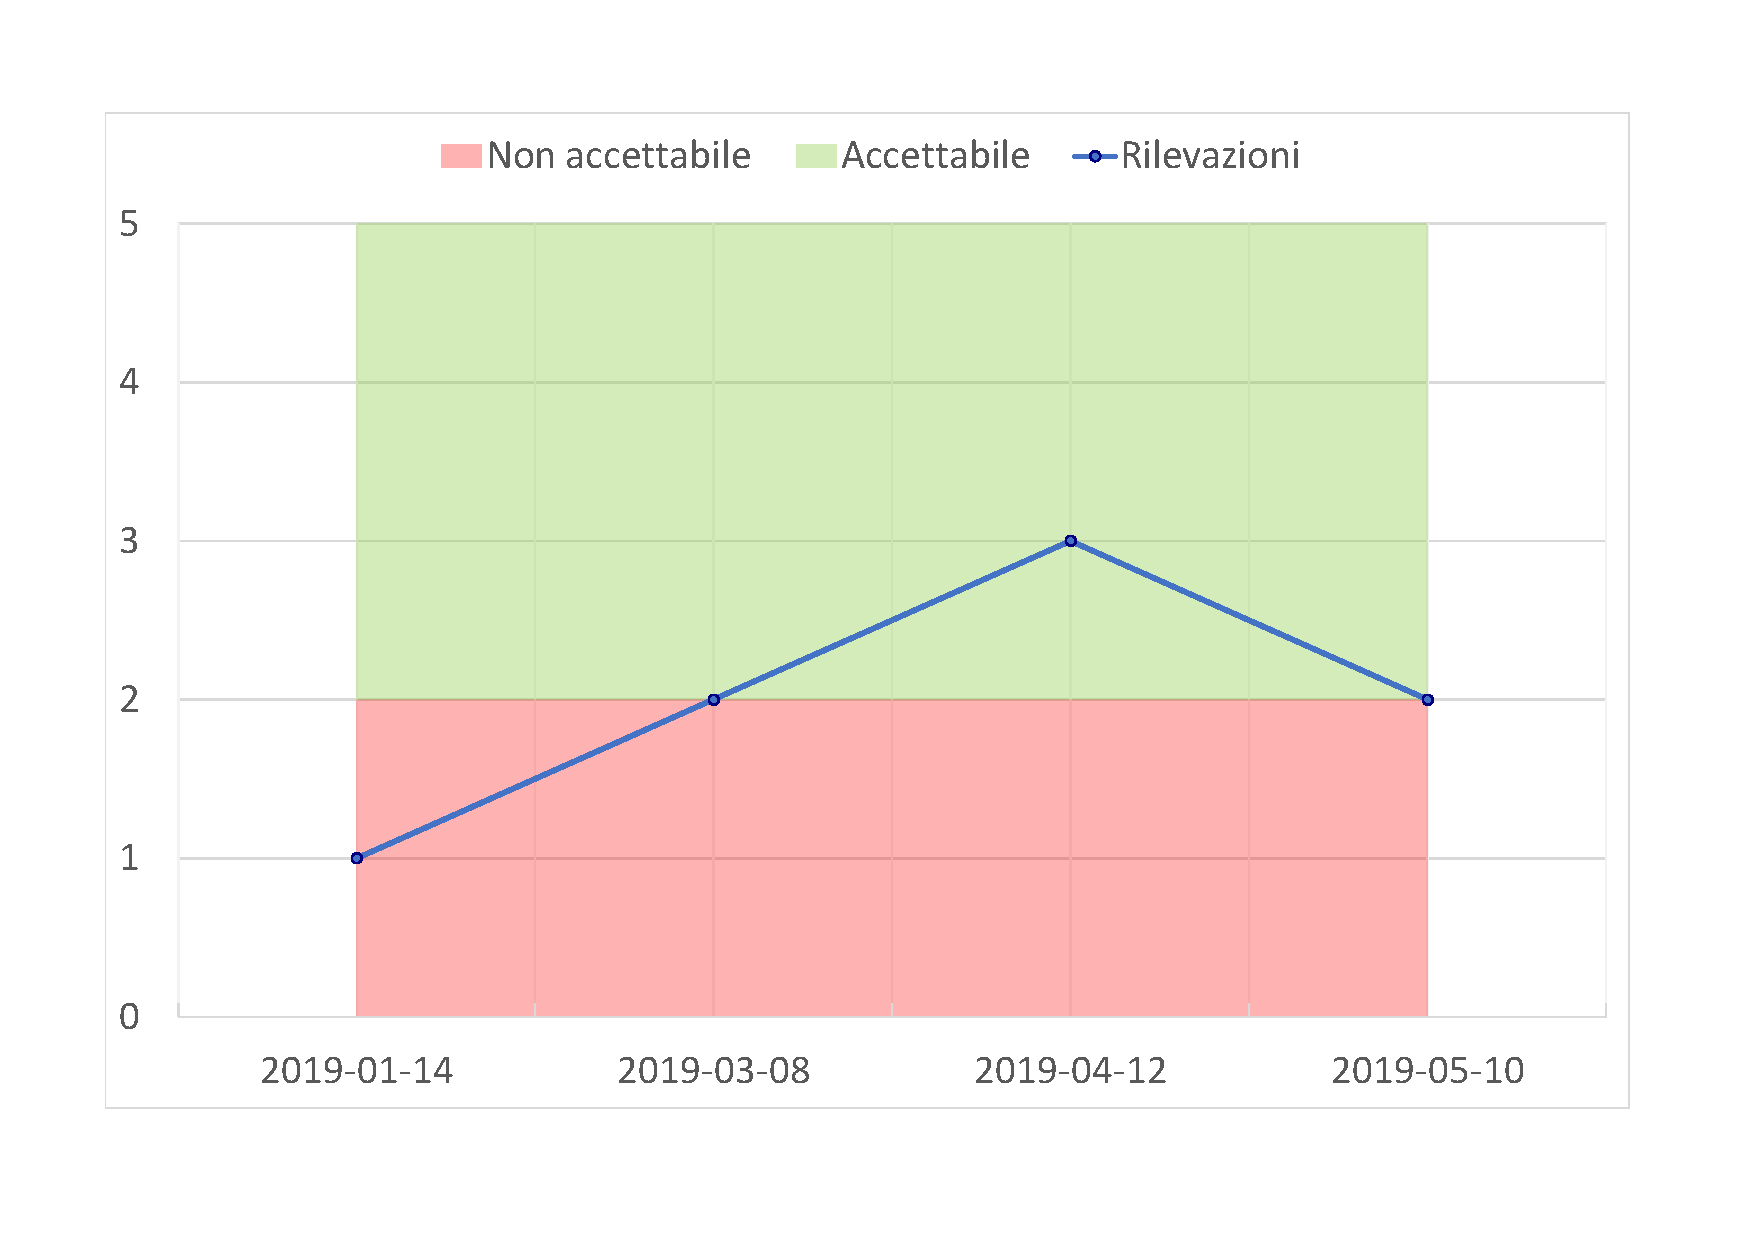
\includegraphics[scale=0.6]{images/resoconto/Analisi.pdf}
	\caption{Valori ISO/IEC 15504 - Analisi dei Requisiti}	
\end{figure}


\begin{figure}[H]
	\centering
	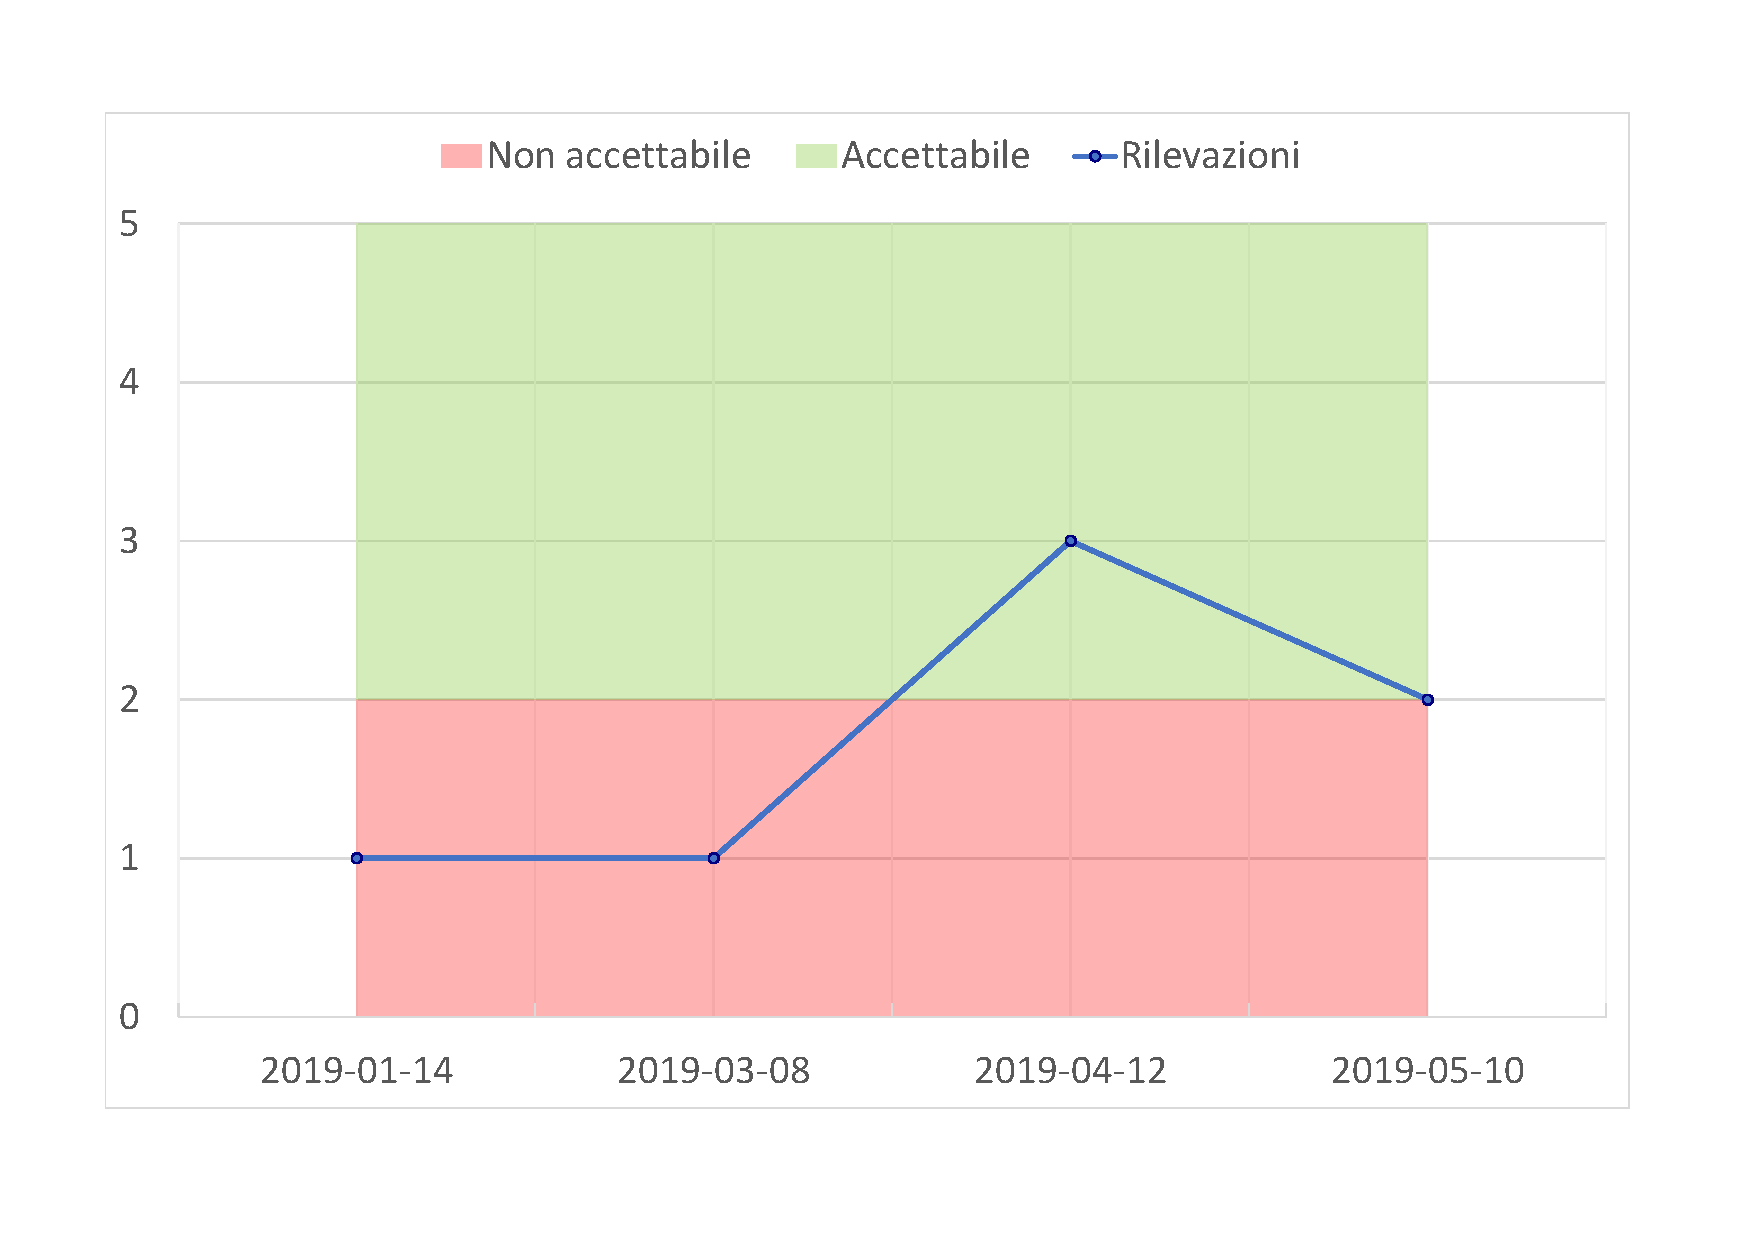
\includegraphics[scale=0.6]{images/resoconto/Normazione.pdf}
	\caption{Valori ISO/IEC 15504 - Normazione}	
\end{figure}


\begin{figure}[H]
	\centering
	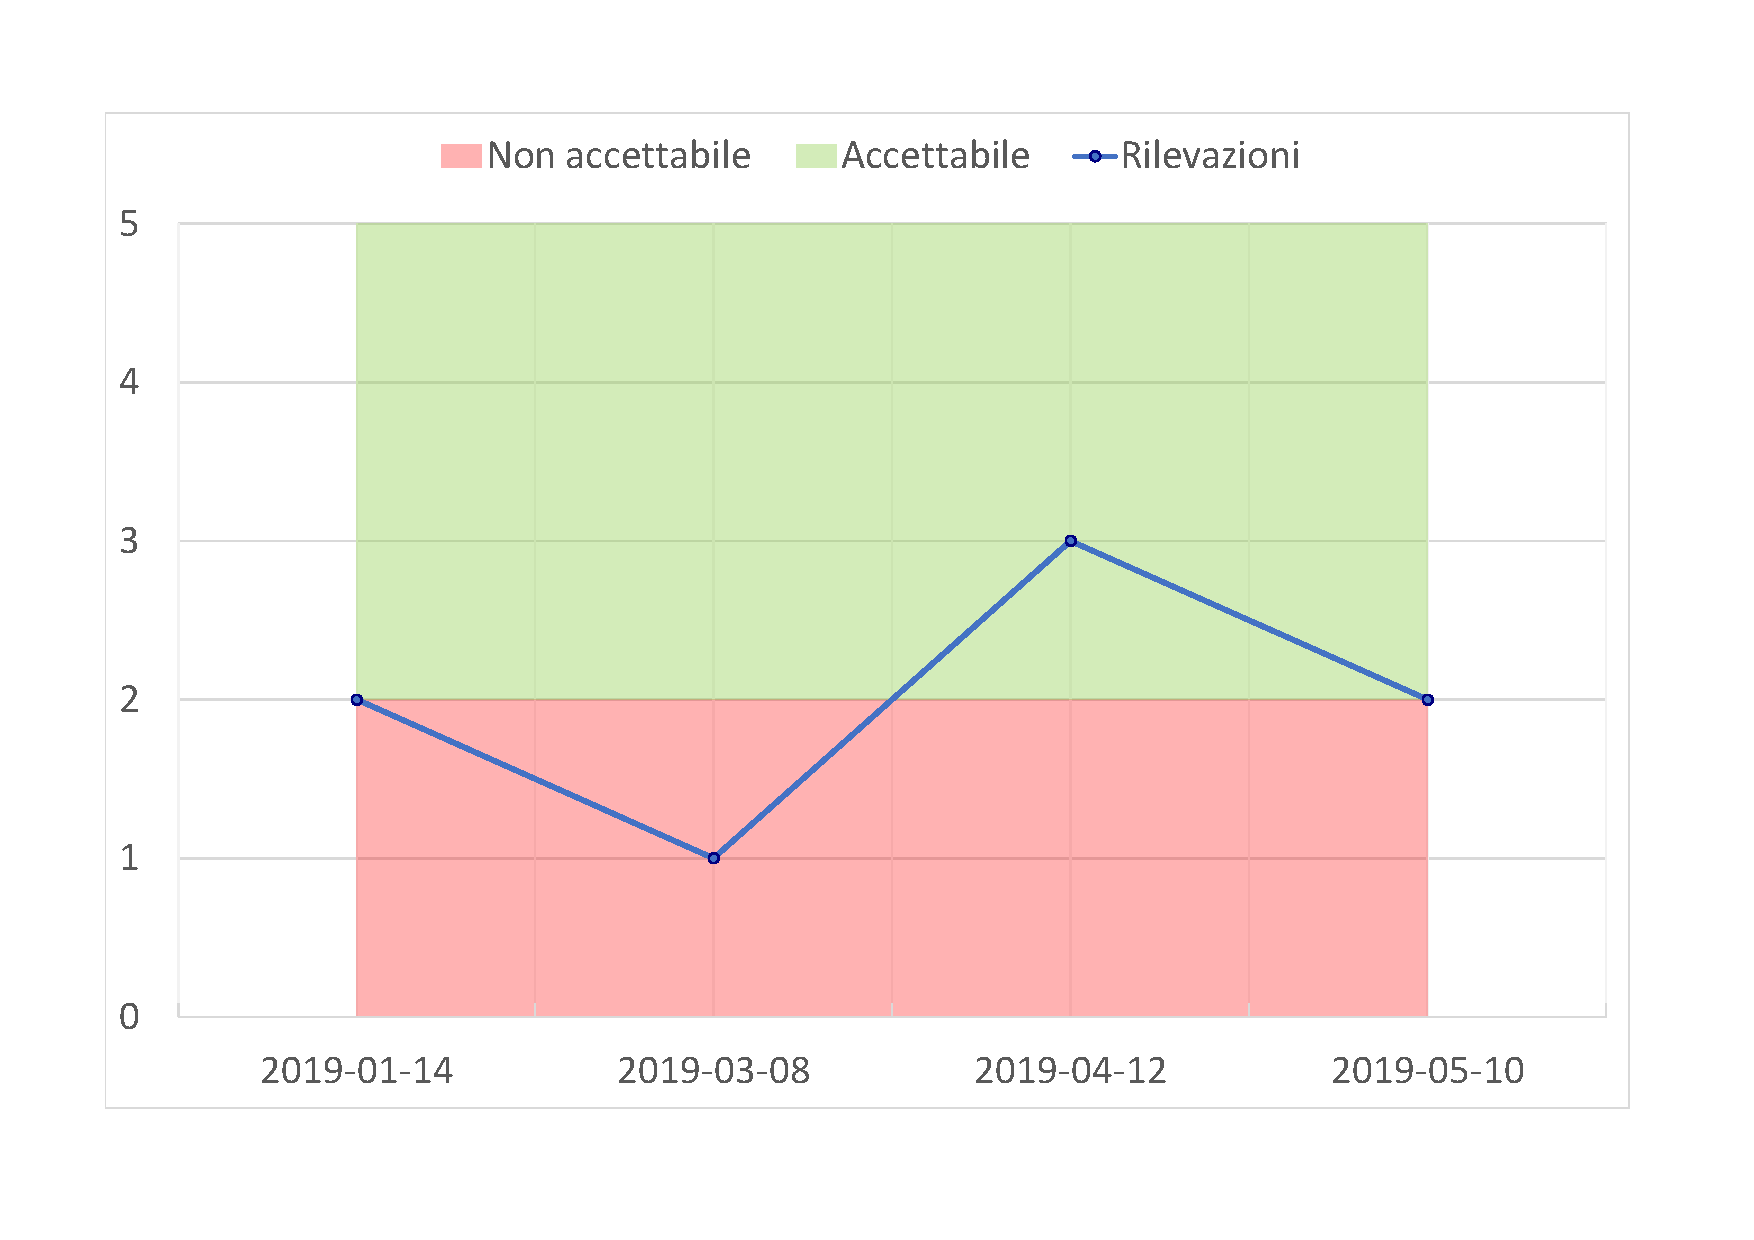
\includegraphics[scale=0.6]{images/resoconto/Pianificazione.pdf}
	\caption{Valori ISO/IEC 15504 - Pianificazione}	
\end{figure}


\begin{figure}[H]
	\centering
	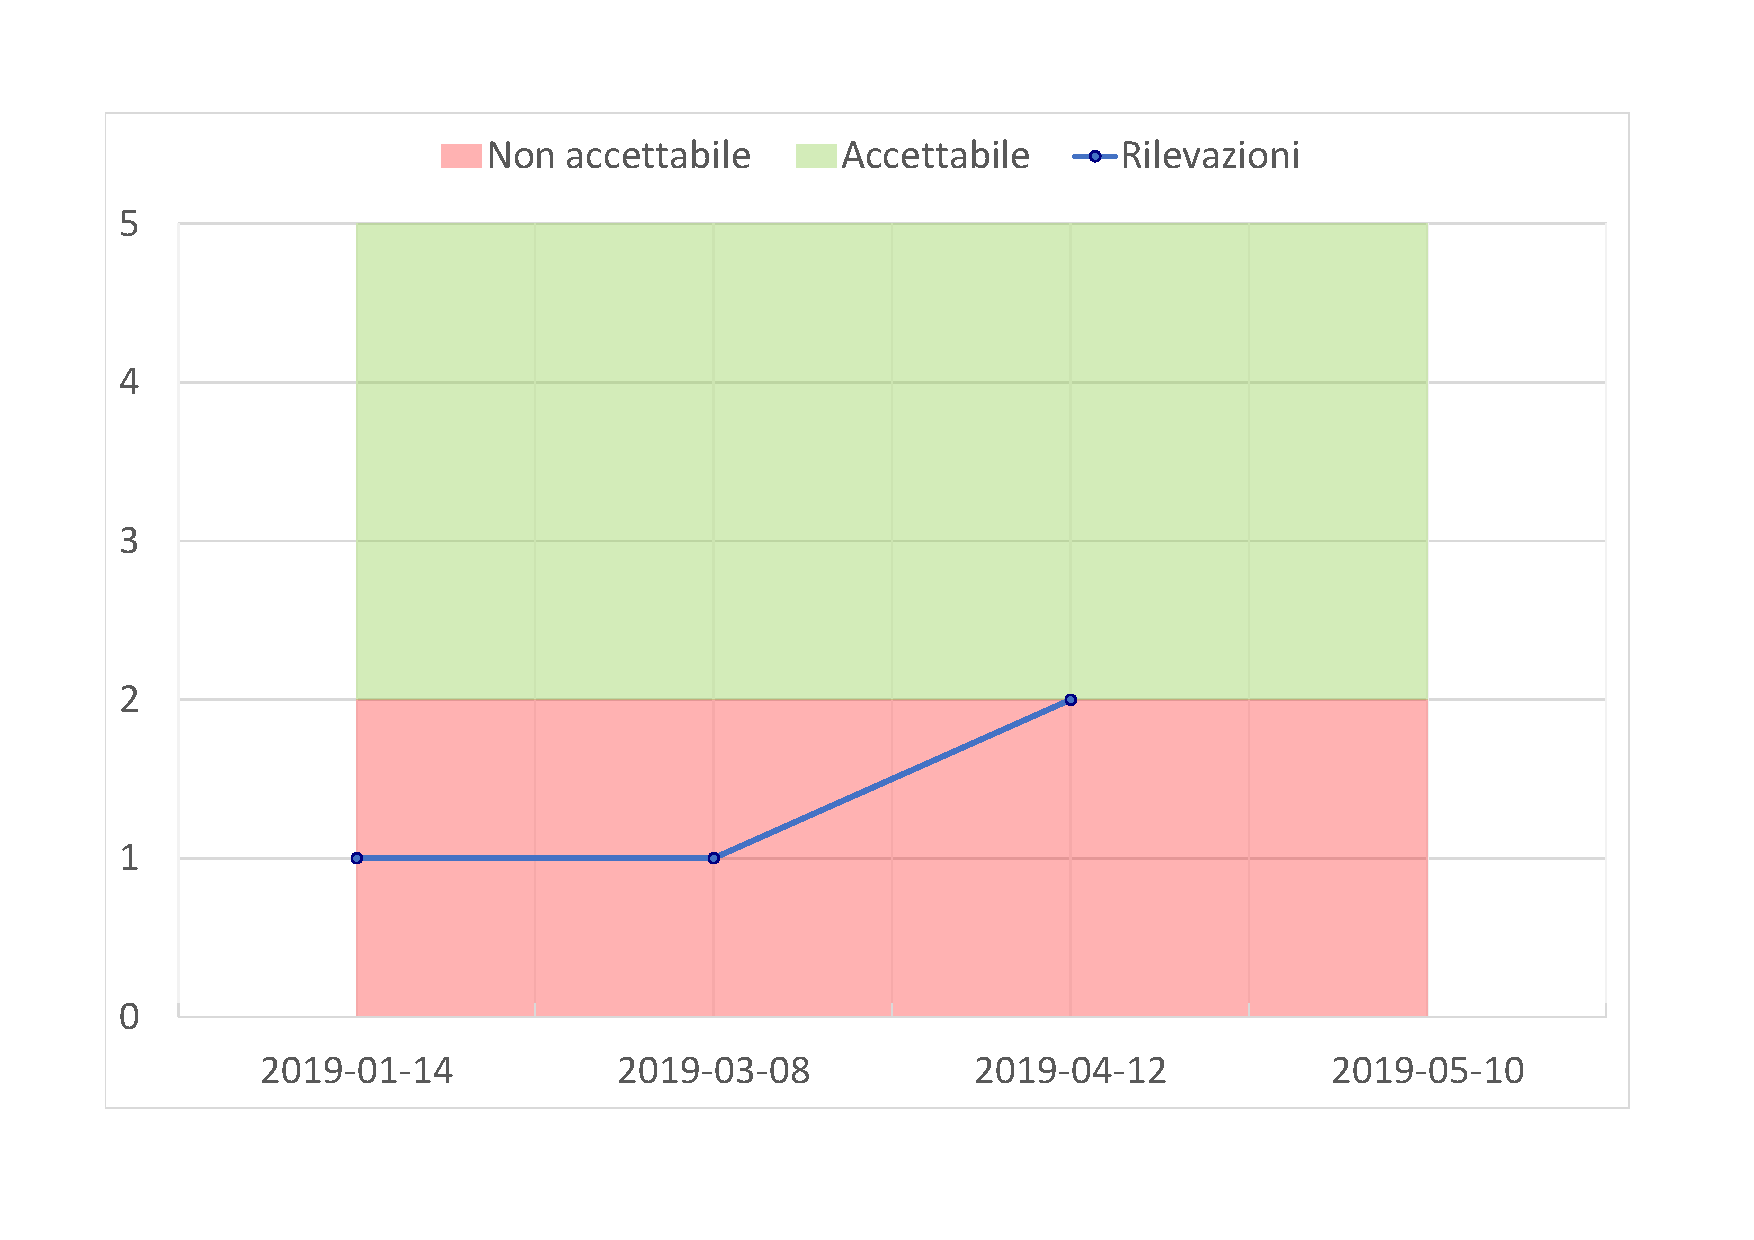
\includegraphics[scale=0.6]{images/resoconto/Progettazione.pdf}
	\caption{Valori ISO/IEC 15504 - Progettazione}	
\end{figure}


\begin{figure}[H]
	\centering
	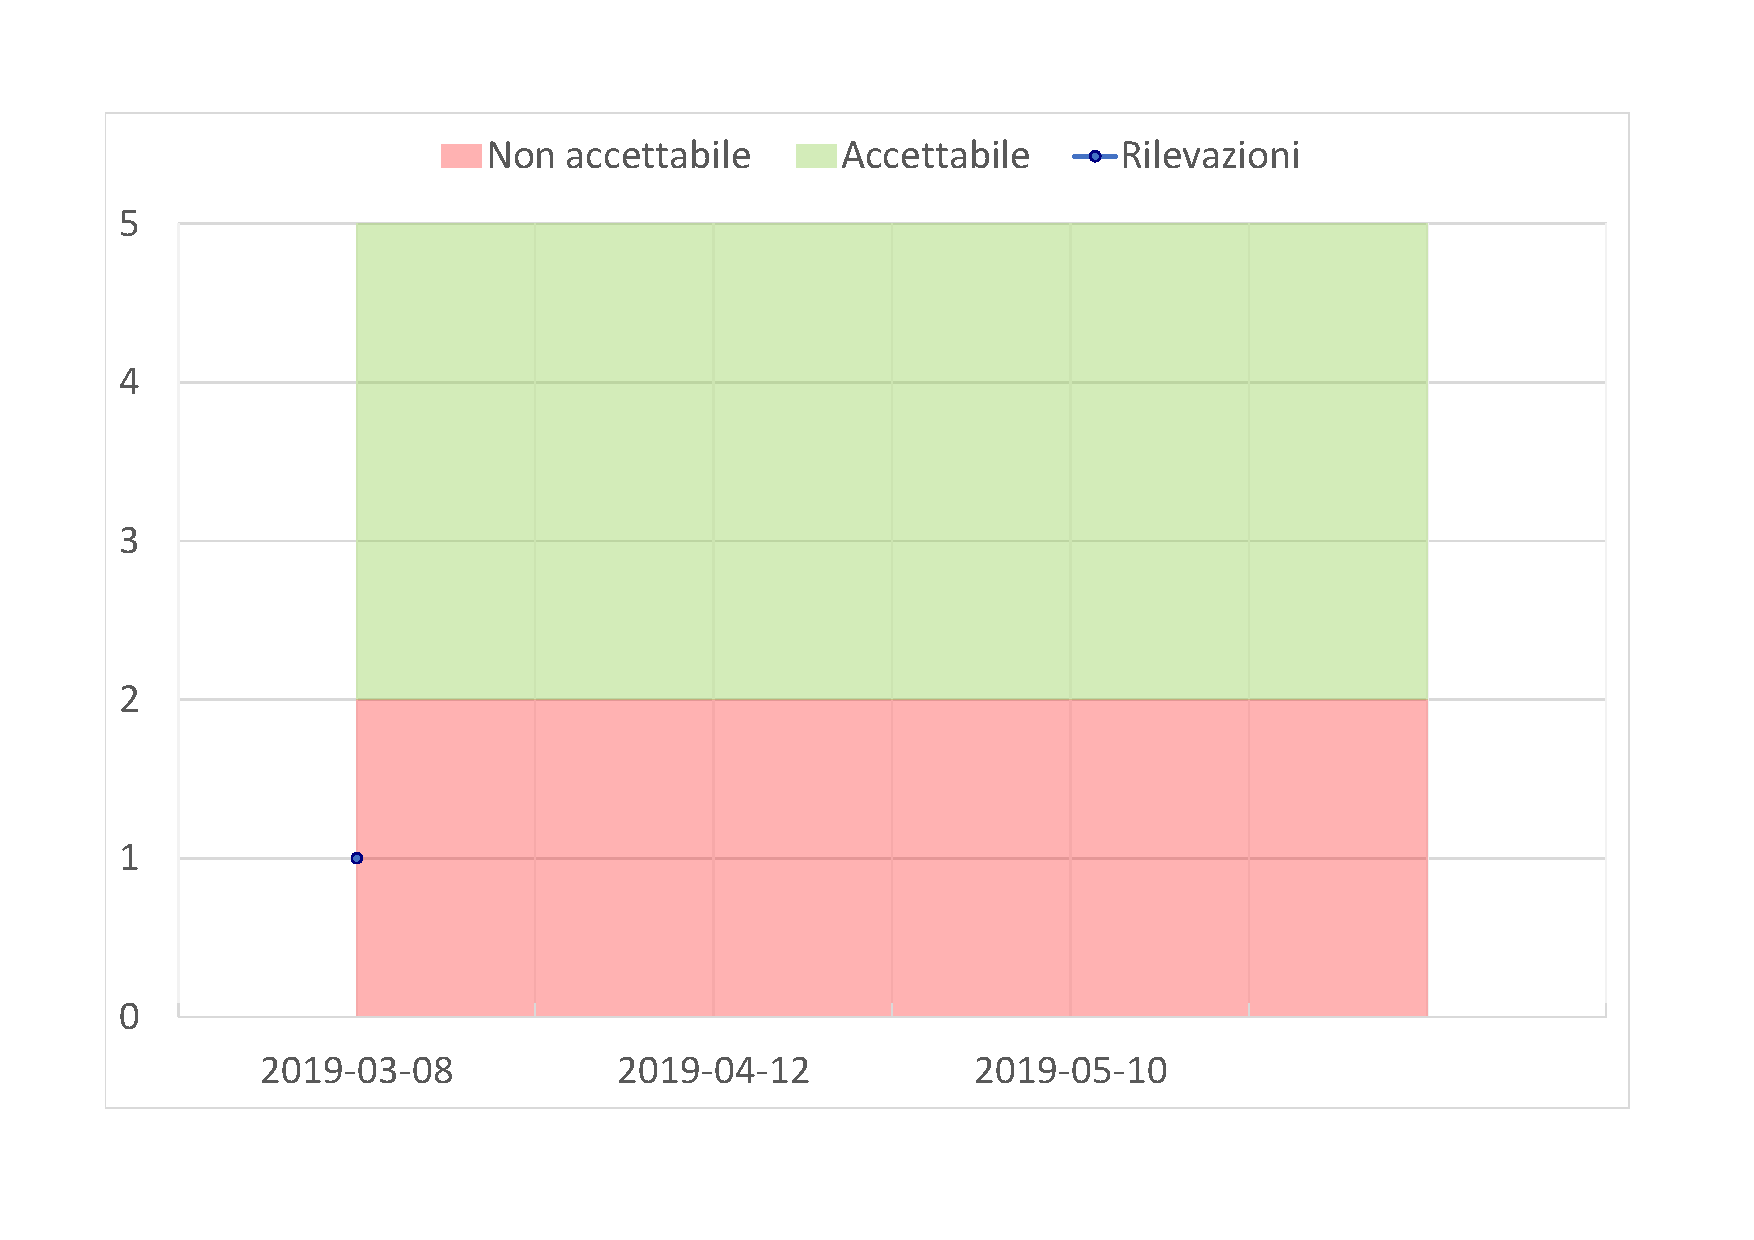
\includegraphics[scale=0.6]{images/resoconto/Ricerca.pdf}
	\caption{Valori ISO/IEC 15504 - Ricerca delle tecnologie}	
\end{figure}


\begin{figure}[H]
	\centering
	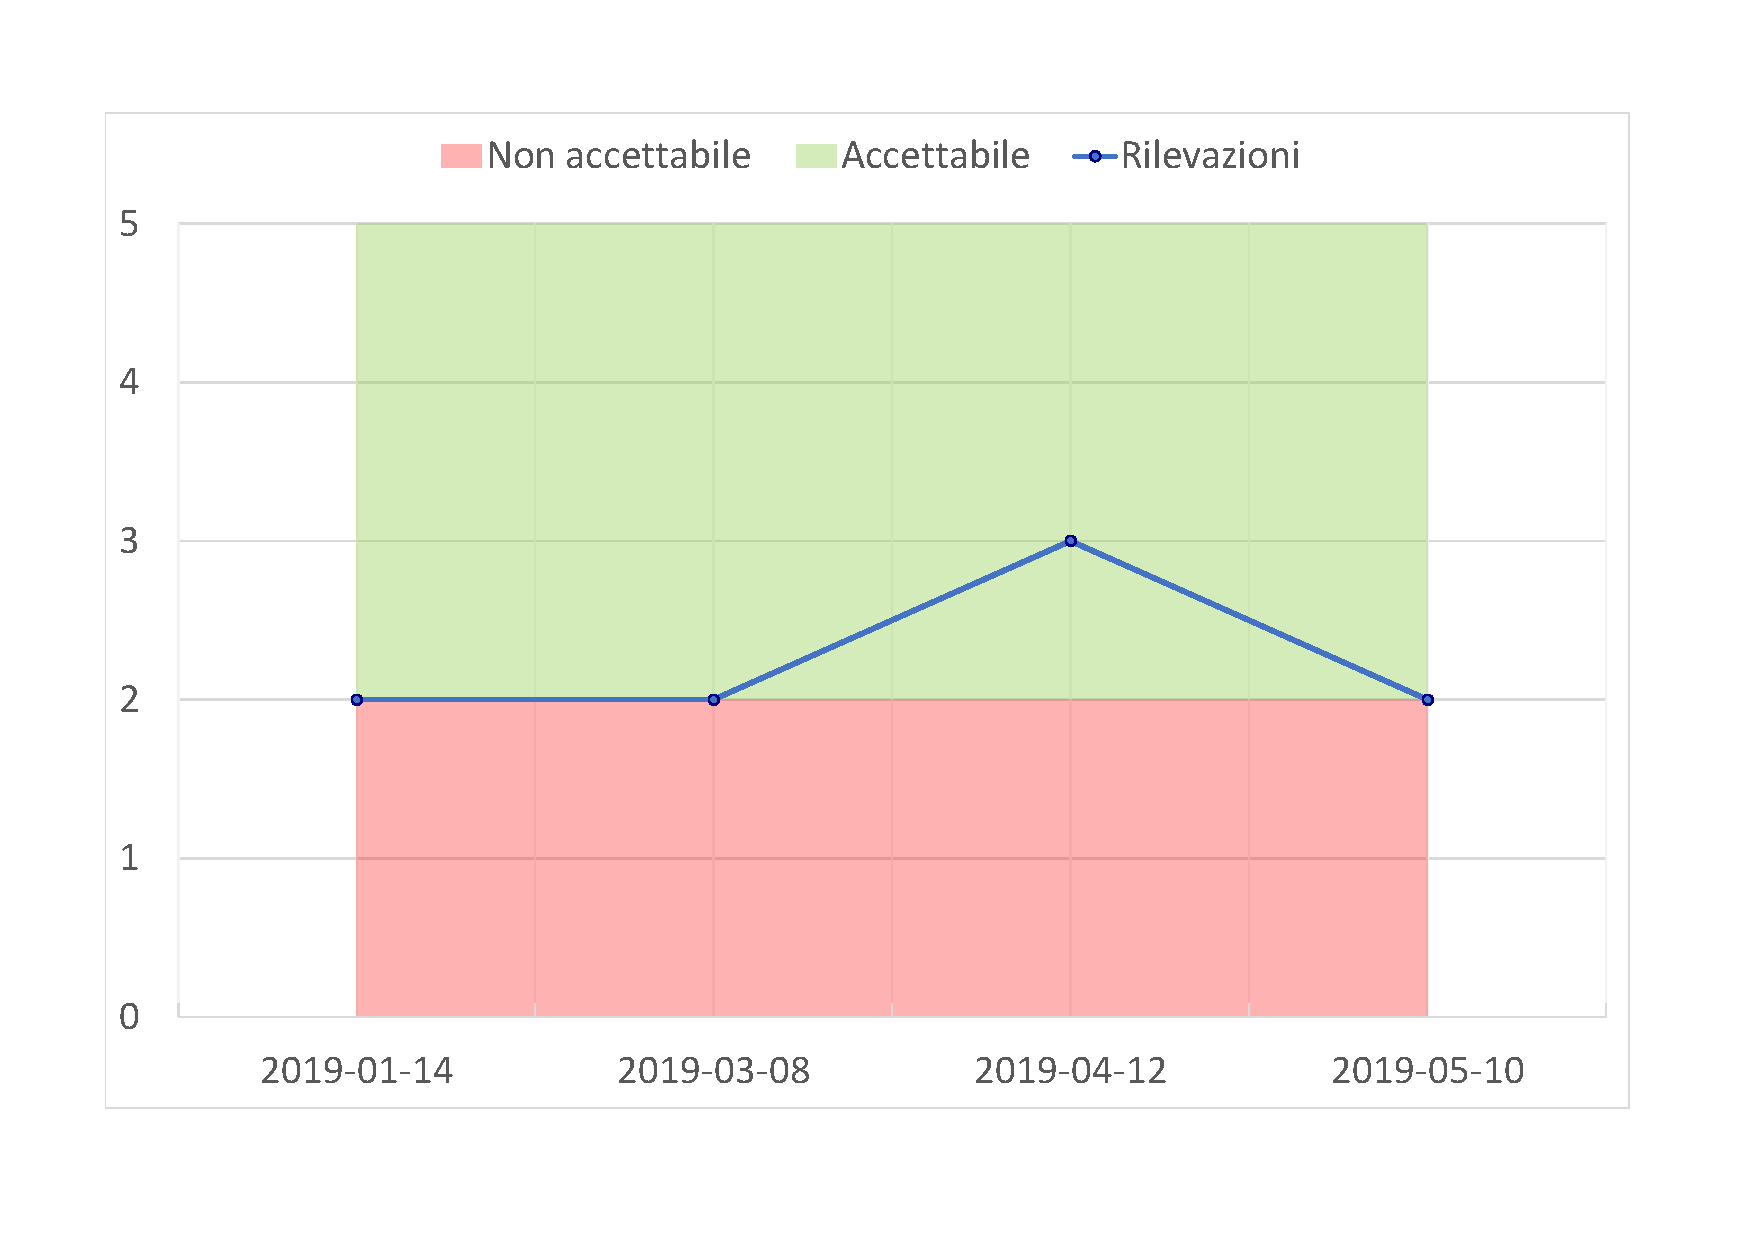
\includegraphics[scale=0.6]{images/resoconto/Documentazione.pdf}
	\caption{Valori ISO/IEC 15504 - Documentazione}	
\end{figure}


\begin{figure}[H]
	\centering
	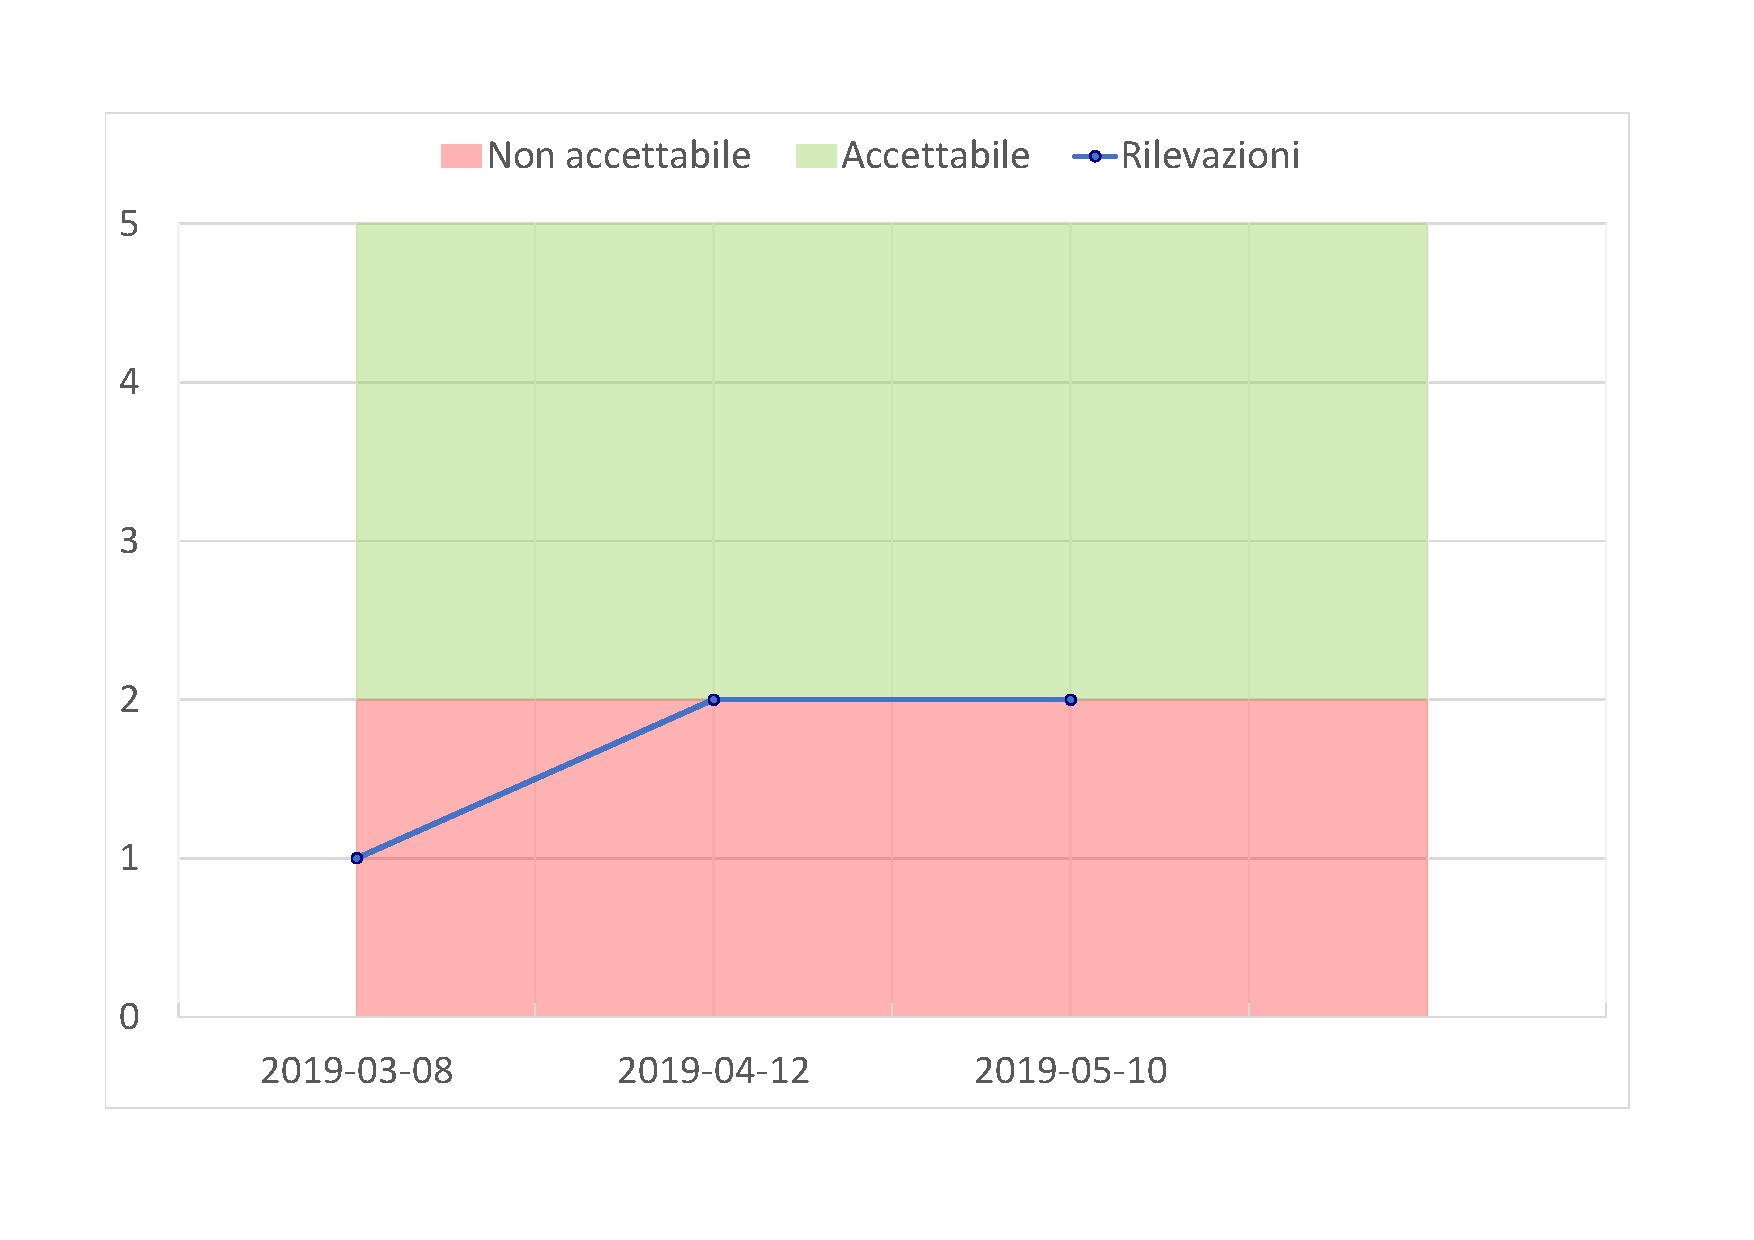
\includegraphics[scale=0.6]{images/resoconto/Codifica.pdf}
	\caption{Valori ISO/IEC 15504 - Codifica}	
\end{figure}
\newpage
\subsubsection{Valori indice RSI - MPC2\\}
Durante lo sviluppo del progetto abbiamo individuato periodicamente tutti i cambiamenti apportati ai requisiti del progetto. Questo ci ha permesso di determinare la stabilità dei requisiti nel tempo grazie all'utilizzo della metrica MPC2.
Riportiamo di seguito i calcoli e le varie rilevazioni effettuate.

\begin{longtable}{>{\centering\arraybackslash}m{3cm} >{\centering\arraybackslash}m{4cm} >{\centering\arraybackslash}m{5cm} >{\centering\arraybackslash}m{2cm}}
	\rowcolor{LightBlue}
	\textbf{\textcolor{white}{Data rilevazioni}}
	& \textbf{\textcolor{white}{Requirement Stability Index (RSI)}}
	& \textbf{\textcolor{white}{Esito}}\\
	
	2019-02-15 & \[1-\frac{0+5+4}{48}=0.81\] & Accettato\\
	\hline
	2019-02-20 & \[1-\frac{5+0+3}{43}=0.81\] & Accettato\\
	\hline
	2019-02-21 & \[1-\frac{8+0+3}{48}=0.77\] & Accettato\\
	\hline
	2019-02-22 & \[1-\frac{5+2+0}{56}=0.85\] & Accettato\\
	\hline
	2019-02-25 & \[1-\frac{11+0+0}{59}=0.81\] & Accettato\\
	\hline
	2019-02-27 & \[1-\frac{10+0+0}{70}=0.88\] & Accettato\\
	\hline
	2019-03-04 & \[1-\frac{12+0+0}{80}=0.86\] & Accettato\\
	\hline
	2019-03-05 & \[1-\frac{14+0+1}{92}=0.83\] & Accettato\\
	\hline\\
	\caption{Rilevazioni indice stabilità requisiti (RSI) - Revisione di progetto}
\end{longtable}

\begin{longtable}{>{\centering\arraybackslash}m{3cm} >{\centering\arraybackslash}m{4cm} >{\centering\arraybackslash}m{5cm} >{\centering\arraybackslash}m{2cm}}
	\rowcolor{LightBlue}
	\textbf{\textcolor{white}{Data rilevazioni}}
	& \textbf{\textcolor{white}{Requirement Stability Index (RSI)}}
	& \textbf{\textcolor{white}{Esito}}\\
	
	2019-03-18 & \[1-\frac{9+0+0}{106}=0.915\] & Accettato\\
	\hline
	2019-03-19 & \[1-\frac{13+0+2}{115}=0.869\] & Accettato\\
	\hline
	\caption{Rilevazioni indice stabilità requisiti (RSI) - Revisione di qualifica}
\end{longtable}

\begin{longtable}{>{\centering\arraybackslash}m{3cm} >{\centering\arraybackslash}m{4cm} >{\centering\arraybackslash}m{5cm} >{\centering\arraybackslash}m{2cm}}
	\rowcolor{LightBlue}
	\textbf{\textcolor{white}{Data rilevazioni}}
	& \textbf{\textcolor{white}{Requirement Stability Index (RSI)}}
	& \textbf{\textcolor{white}{Esito}}\\
	2019-04-30 & \[1-\frac{2+3+0}{128}=0.960\] & Accettato\\
	\hline
	2019-05-07 & \[1-\frac{0+2+0}{127}=0.984\] & Accettato\\
	\hline
	\caption{Rilevazioni indice stabilità requisiti (RSI) - Revisione di accettazione}
\end{longtable}

\begin{figure}[H]
	\centering
	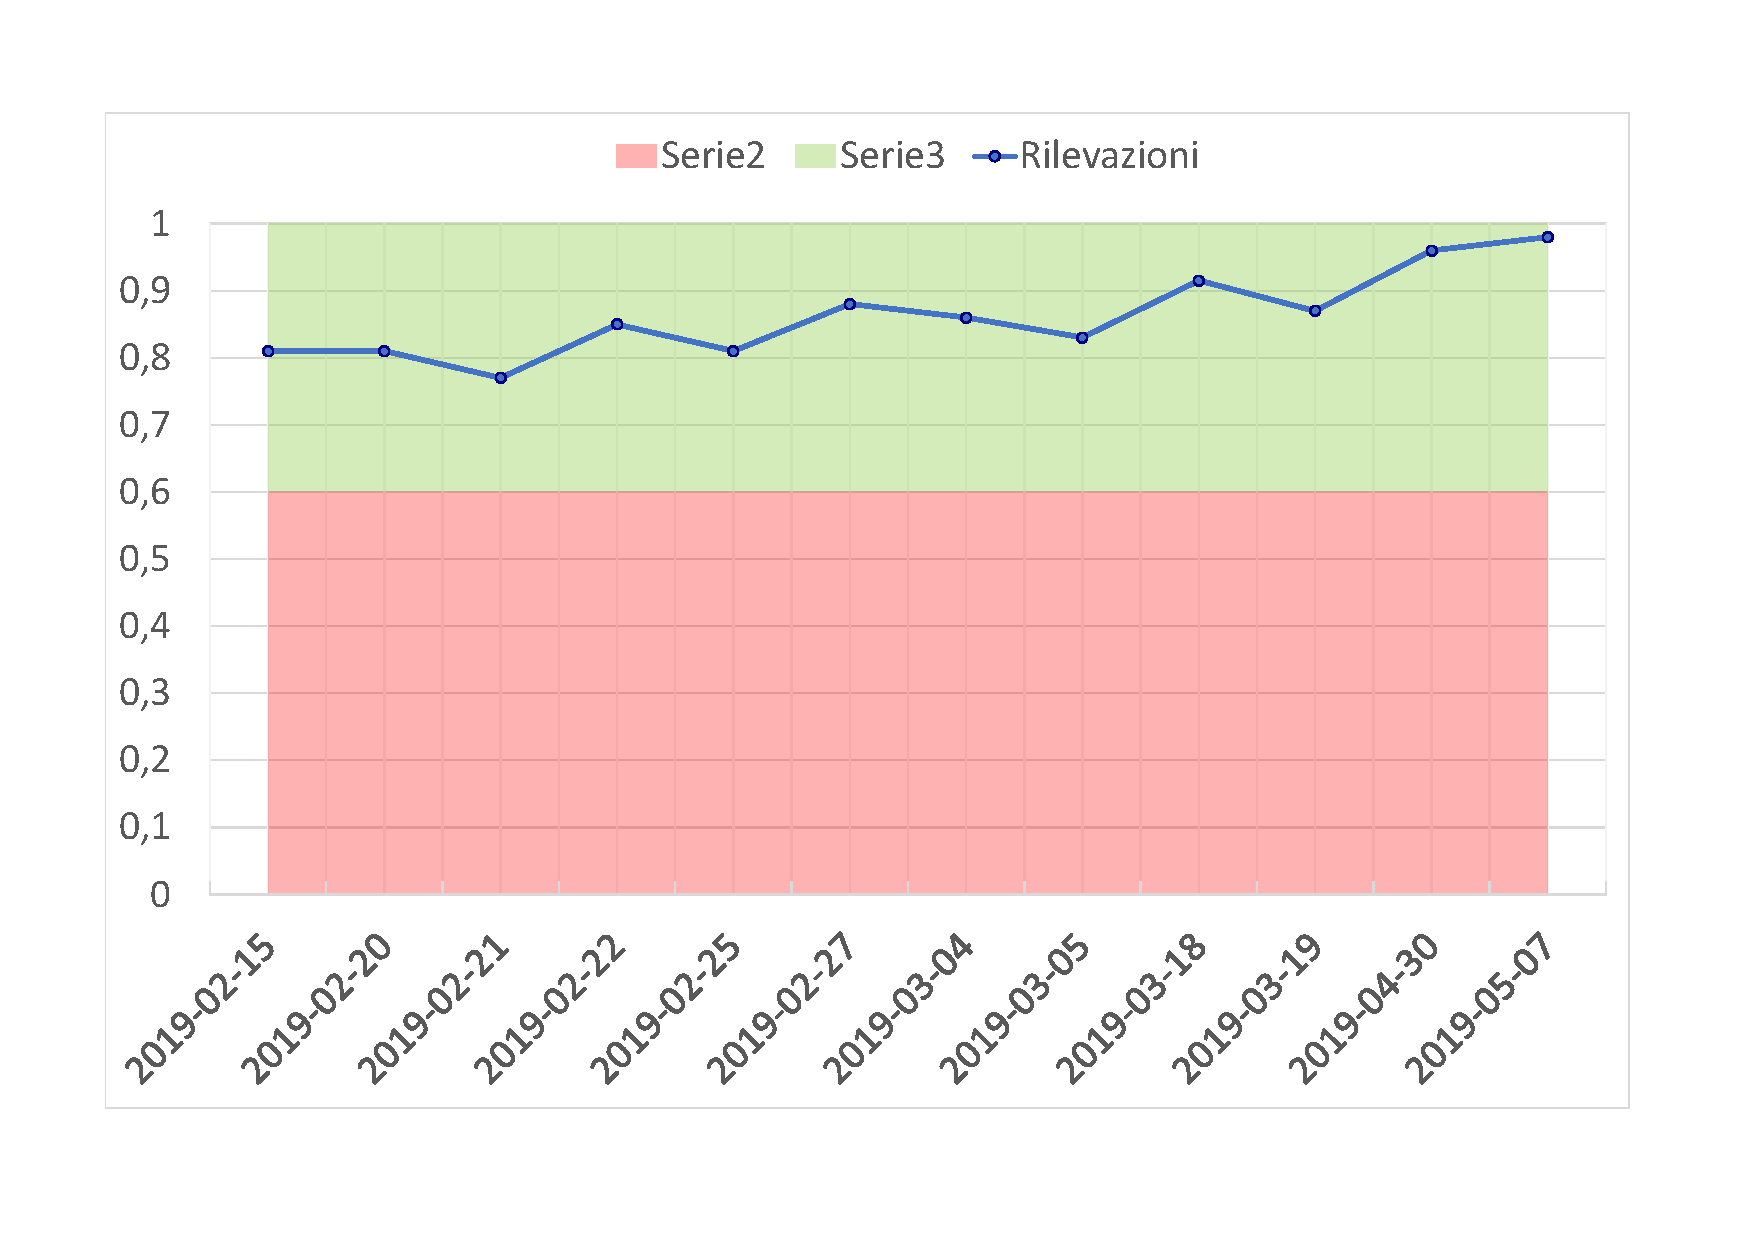
\includegraphics[scale=0.6]{images/resoconto/MPC2Chart.pdf}
	\caption{Serie storica rilevazioni stabilità requisiti}	
\end{figure}


\subsubsection{Violazione dello stile di codifica - MPC3}

\subparagraph{Codifica al 2019-04-05}
In questo periodo dell'attività di codifica, sono state commesse 20 violazioni dello stile di codifica, così distribuite:
 \begin{itemize}
 	\item \textbf{Utilizzo lingua inglese}: 13 violazioni.
 	\item \textbf{Utilizzo TSLint}: 0 violazioni.
 	\item \textbf{Lunghezza linee di codice}: 2 violazioni.
 	\item \textbf{Nomenclatura}: 0 violazioni.
 	\item \textbf{Commenti al codice}: 5 violazioni.
 \end{itemize}
Questi dati non sono accettabili, il gruppo si impegnerà a correggere le violazioni nel prossimo periodo di codifica.

\subparagraph{Codifica al 2019-04-12}
In questo periodo dell'attività di codifica, sono state commesse 7 violazioni dello stile di codifica, così distribuite:
 \begin{itemize}
 	\item \textbf{Utilizzo lingua inglese}: 0 violazioni.
 	\item \textbf{Utilizzo TSLint}: 0 violazioni.
 	\item \textbf{Lunghezza linee di codice}: 7 violazioni.
 	\item \textbf{Nomenclatura}: 0 violazioni.
 	\item \textbf{Commenti al codice}: 0 violazioni.
 \end{itemize}
Lo stile di codifica è migliorato rispetto alla precedente rilevazione. Tuttavia l'obbiettivo di avere un numero inferiore alle 10 violazioni è rispettato ma ancora migliorabile.

\subparagraph{Codifica al 2019-04-19}
In questo periodo dell'attività di codifica, sono state commesse 7 violazioni dello stile di codifica, così distribuite:
 \begin{itemize}
 	\item \textbf{Utilizzo lingua inglese}: 0 violazioni.
 	\item \textbf{Utilizzo TSLint}: 0 violazioni.
 	\item \textbf{Lunghezza linee di codice}: 3 violazioni.
 	\item \textbf{Nomenclatura}: 0 violazioni.
 	\item \textbf{Commenti al codice}: 0 violazioni.
 \end{itemize}
Lo stile di codifica è migliorato rispetto alla precedente rilevazione. Tuttavia l'obbiettivo di avere un numero inferiore alle 10 violazioni è rispettato ma ancora migliorabile.

\subparagraph{Codifica al 2019-04-26}
In questo periodo dell'attività di codifica, sono state commesse 7 violazioni dello stile di codifica, così distribuite:
 \begin{itemize}
 	\item \textbf{Utilizzo lingua inglese}: 0 violazioni.
 	\item \textbf{Utilizzo TSLint}: 0 violazioni.
 	\item \textbf{Lunghezza linee di codice}: 6 violazioni.
 	\item \textbf{Nomenclatura}: 0 violazioni.
 	\item \textbf{Commenti al codice}: 0 violazioni.
 \end{itemize}
Lo stile di codifica è migliorato rispetto alla precedente rilevazione. Tuttavia l'obbiettivo di avere un numero inferiore alle 10 violazioni è rispettato ma ancora migliorabile.

\subparagraph{Codifica al 2019-05-03}
In questo periodo dell'attività di codifica, sono state commesse 7 violazioni dello stile di codifica, così distribuite:
 \begin{itemize}
 	\item \textbf{Utilizzo lingua inglese}: 0 violazioni.
 	\item \textbf{Utilizzo TSLint}: 3 violazioni.
 	\item \textbf{Lunghezza linee di codice}: 5 violazioni.
 	\item \textbf{Nomenclatura}: 0 violazioni.
 	\item \textbf{Commenti al codice}: 0 violazioni.
 \end{itemize}
Lo stile di codifica è migliorato rispetto alla precedente rilevazione. Tuttavia l'obbiettivo di avere un numero inferiore alle 10 violazioni è rispettato.

\subparagraph{Codifica al 2019-05-10}
In questo periodo non si è verificata l'attività di codifica in quanto il prodotto è stato ritenuto concluso precedentemente.

\begin{figure}[H]
	\centering
	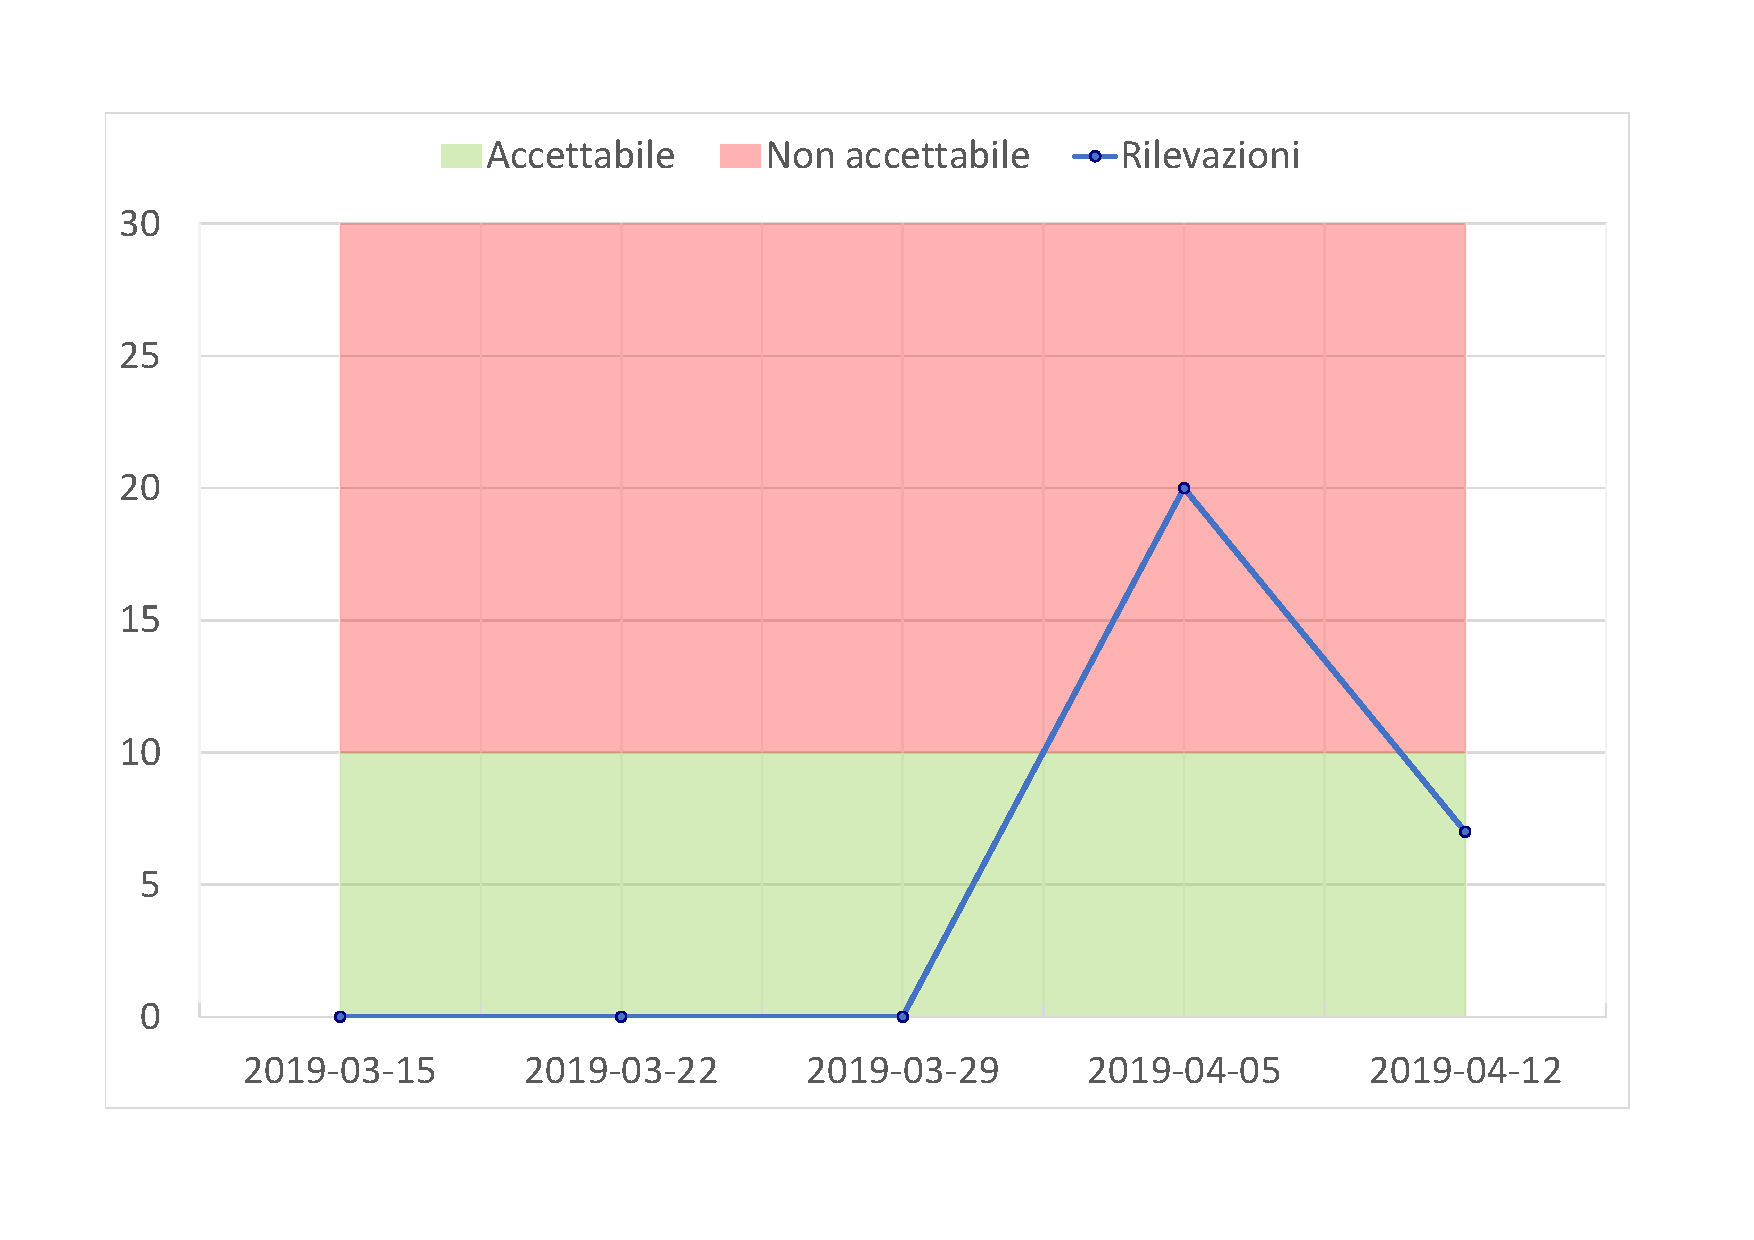
\includegraphics[scale=0.6]{images/resoconto/MPC3Chart.pdf}
	\caption{Serie storica numero di violazioni dello stile di codifica}	
\end{figure}

\subsubsection{Test di integrazione implementati - MPC4}
\subparagraph{Codifica al 2019-04-05}
In questo periodo dell'attività di codifica, è stato implementato 1 test di integrazione su un totale di 10 test di integrazione preventivati.
Nonostante non raggiunga il livello di accettazione della
metrica, questo risultato è ritenuto sufficiente a questo punto del progetto poiché sono previsti altri incrementi alla codifica che porteranno all'implementazione di altri test.

\subparagraph{Codifica al 2019-04-12}
In questo periodo dell'attività di codifica, sono stati implementati 3 test di integrazione per un totale di 4 coprendo il 40\% dei test di integrazione preventivati.
Nonostante non raggiunga il livello di accettazione della
metrica, questo risultato è ritenuto sufficiente a questo punto del progetto poiché sono previsti altri incrementi alla codifica che porteranno all'implementazione di altri test. 

\subparagraph{Codifica al 2019-04-19}
In questo periodo dell'attività di codifica, sono stati implementati 2 test di integrazione per un totale di 6 coprendo il 60\% dei test di integrazione preventivati.
Nonostante non raggiunga il livello di accettazione della
metrica, questo risultato è ritenuto sufficiente a questo punto del progetto poiché sono previsti altri incrementi alla codifica che porteranno all'implementazione di altri test. 

\subparagraph{Codifica al 2019-04-26}
In questo periodo dell'attività di codifica, sono stati implementati 2 test di integrazione per un totale di 8 coprendo il 80\% dei test di integrazione preventivati.
Nonostante non raggiunga il livello di accettazione della
metrica, questo risultato è ritenuto sufficiente a questo punto del progetto poiché sono previsti altri incrementi alla codifica che porteranno all'implementazione di altri test. 

\subparagraph{Codifica al 2019-05-03}
In questo periodo dell'attività di codifica, sono stati implementati 3 test di integrazione per un totale di 9 coprendo il 90\% dei test di integrazione preventivati.
A seguito di questo periodo di codifica la soglia di accettabilità della metrica è stata raggiunta.
Il gruppo si impegnerà ad implementare ulteriori test di integrazione.


\subparagraph{Codifica al 2019-05-10}
In questo periodo dell'attività di codifica, sono stati implementati 1 test di integrazione per un totale di 10 coprendo il 100\% dei test di integrazione preventivati.

sakdjhaskjdhskjdh
\\
\\
Riportiamo di seguito una tabella rappresentativa dello stato di avanzamento dei test. La tabella verrà aggiornata alla fine di ogni periodo dell'attività di codifica.

	\begin{longtable}{|>{\centering\arraybackslash}m{1.6cm}|>{\centering\arraybackslash}m{6.41cm}|>{\centering\arraybackslash}m{3.1cm}|}		
	\rowcolor{LightBlue}
	\textbf{\textcolor{white}{Test}}
	& \textbf{\textcolor{white}{Stato}}
	& \textbf{\textcolor{white}{Esito}}\\
	\hline
	TI1
	& Implementato & Superato
	\\ \hline
	\rowcolor{LightGray}
	TI2
	& Implementato & Superato
	\\ \hline
	TI3
	& Implementato & Superato
	\\ \hline
	\rowcolor{LightGray}
	TI4
	& Implementato & Superato
	\\ \hline
	TI5
	& Implementato & Superato
	\\ \hline
	\rowcolor{LightGray}
	TI6
	& Implementato & Superato
	\\ \hline	
	TI7
	& Implementato & Superato
	\\ \hline	
	\rowcolor{LightGray}
	TI8
	& Implementato & Superato
	\\ \hline	
	TI9
	& Implementato & Superato
	\\ \hline	
	\rowcolor{LightGray}
	TI10
	& Implementato & Superato
	\\ \hline	
	\caption{Test di integrazione - stato di avanzamento}
\end{longtable}

\begin{figure}[H]
	\centering
	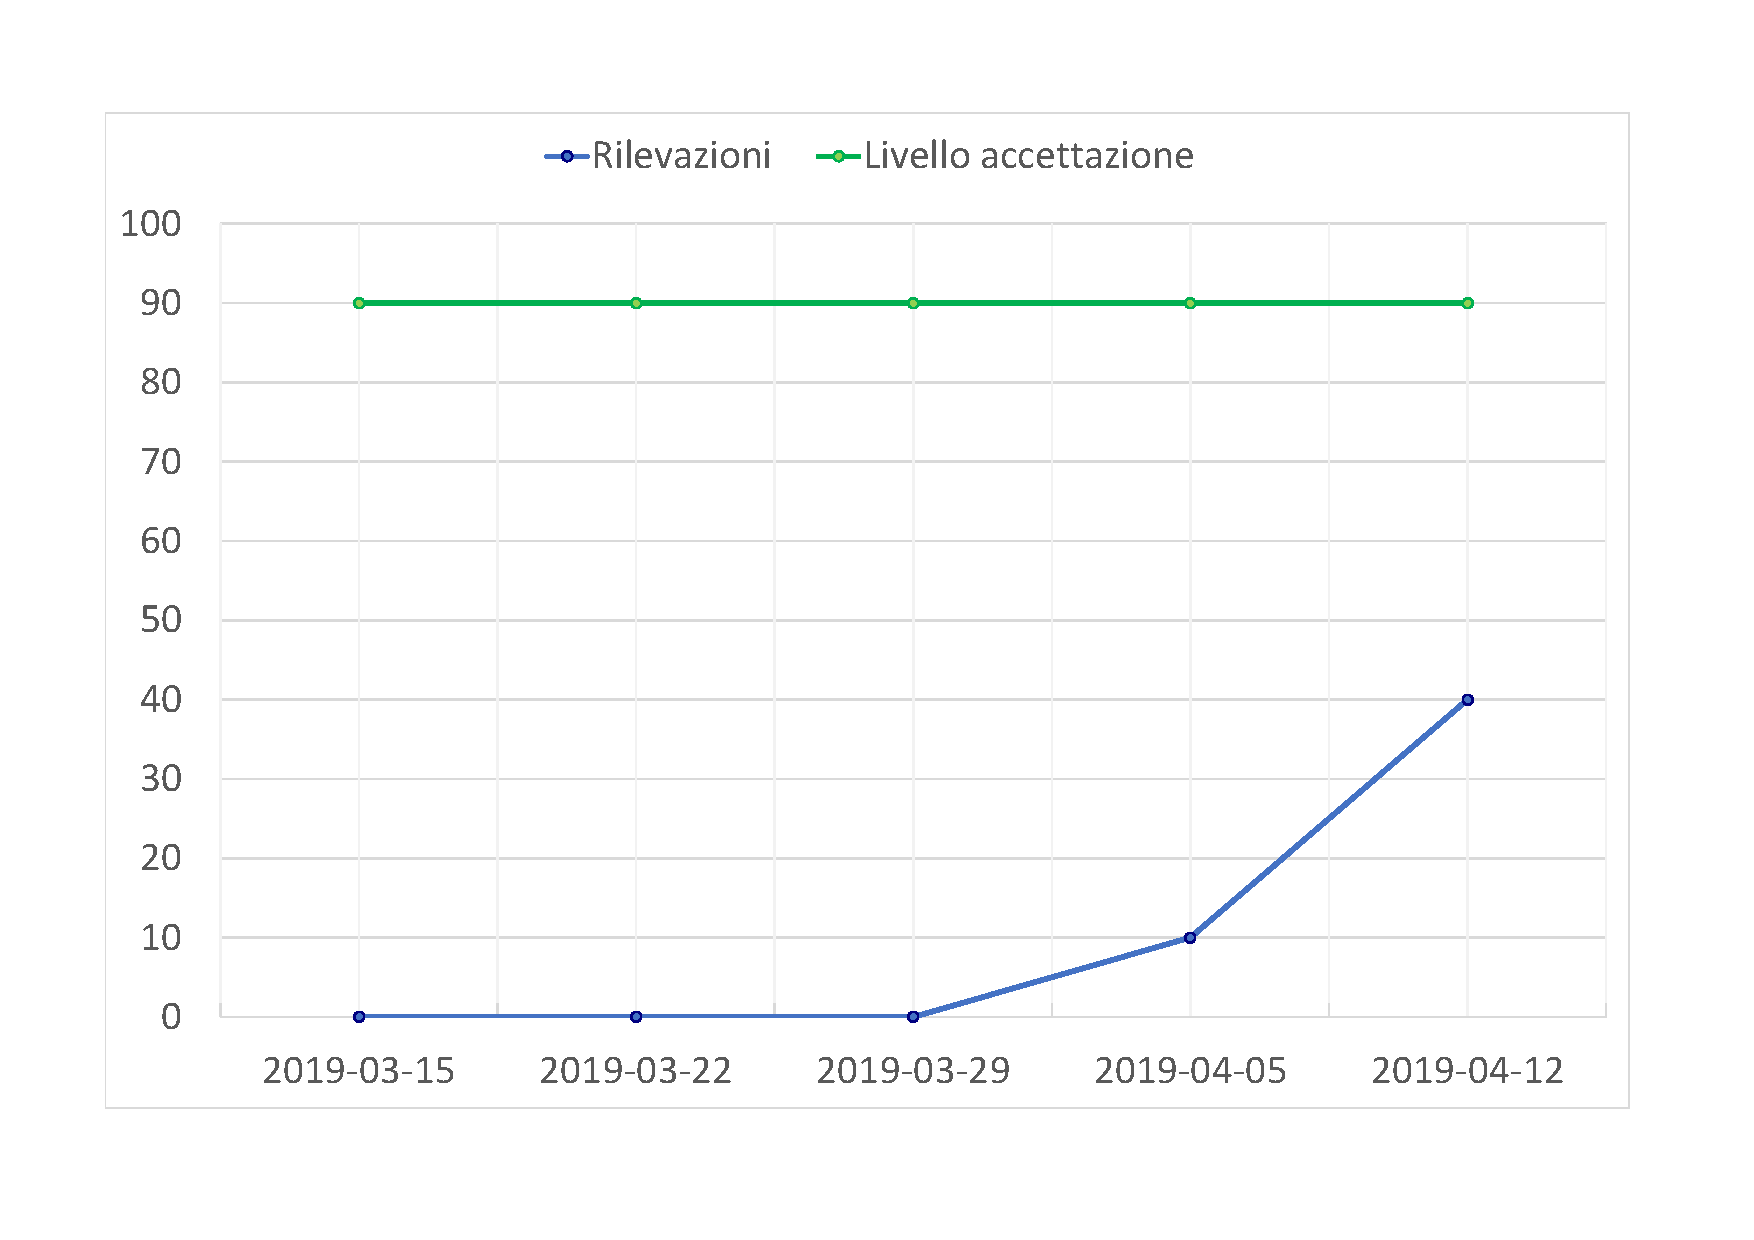
\includegraphics[scale=0.6]{images/resoconto/MPC4Chart.pdf}
	\caption{Serie storica linee di codice per procedura}	
\end{figure}

\subsubsection{Test di sistema implementati - MPC5}
\subparagraph{Codifica al 2019-04-19}


\subparagraph{Codifica al 2019-04-26}


\subparagraph{Codifica al 2019-05-03}


\subparagraph{Codifica al 2019-05-10}


\begin{longtable}{|>{\centering\arraybackslash}m{1.6cm}|>{\centering\arraybackslash}m{6.41cm}|>{\centering\arraybackslash}m{3.1cm}|}		
	\rowcolor{LightBlue}
	\textbf{\textcolor{white}{Test}}
	& \textbf{\textcolor{white}{Stato}}
	& \textbf{\textcolor{white}{Esito}}\\
	\hline
		\rowcolor{LightGray}
		TS-RO1
		& Implementato
		& Superato
		\\ \hline
		\rowcolor{white}
		TS-RO2
		& Implementato
		& Superato
		\\ \hline
		\rowcolor{LightGray}
		TS-RD1
		& Implementato
		& Superato
		\\ \hline
		\rowcolor{white}
		TS-RD2
		& Non implementato
		& Non superato 
		\\ \hline
		\rowcolor{LightGray}
		TS-RO3
		& Implementato
		& Superato
		\\ \hline
		\rowcolor{white}
		TS-RO4		
		& Implementato
		& Superato
		\\ \hline
		\rowcolor{LightGray}
		TS-RP1		
		& Non implementato
		& Non superato	
		\\ \hline
		\rowcolor{LightGray}
		TS-RP2		
		& Non implementato
		& Non superato	
		\\ \hline
		\rowcolor{white}
		TS-RP3		
		& Implementato
		& Superato
		\\ \hline
		\rowcolor{LightGray}
		TS-RD3		
		& Implementato
		& Superato
		\\ \hline
		\rowcolor{white}
		TS-RP4		
		& Implementato
		& Superato
		\\ \hline
		\rowcolor{LightGray}
		TS-RP5		
		& Implementato
		& Superato
		\\ \hline
		\rowcolor{white}
		TS-RO5		
		& Implementato
		& Superato
		\\ \hline
		\rowcolor{LightGray}
		TS-RO6		
		& Implementato
		& Superato
		\\ \hline
		\rowcolor{white}
		TS-RD4		
		& Implementato
		& Superato
		\\ \hline
		\rowcolor{LightGray}
		TS-RP6		
		& Non implementato
		& Non superato
		\\ \hline
		\rowcolor{white}
		TS-RP7		
		& Non implementato
		& Non superato
		\\ \hline
		\rowcolor{LightGray}
		TS-RO7		v
		\\ \hline
		\rowcolor{white}
		TS-RO8		
		& Implementato
		& Superato
		\\ \hline
		\rowcolor{LightGray}
		TS-RO9		
		& Implementato
		& Superato
		\\ \hline
		\rowcolor{white}
		TS-RD5		v
		\\ \hline
		\rowcolor{LightGray}
		TS-RD6		
		& Implementato
		& Superato
		\\ \hline
		\rowcolor{white}
		TS-RD7
		& Implementato
		& Superato
		\\ \hline
		\rowcolor{LightGray}
		TS-RD8		
		& Non implementato
		& Non superato
		\\ \hline 
		\rowcolor{white}
		TS-RP8		
		& Implementato
		& Superato		
		\\ \hline
		\rowcolor{LightGray}
		TS-RP9		
		& Implementato
		& Superato
		\\ \hline
		\rowcolor{white}
		TS-RO10
		& Implementato
		& Superato
		\\ \hline
		\rowcolor{LightGray}
		TS-RP10		
		& Non implementato
		& Non superato
		\\ \hline
		\rowcolor{white}
		TS-RP11		
		& Implementato
		& Superato
		\\ \hline
		\rowcolor{LightGray}
		TS-RP12		
		& Non implementato
		& Non superato
		\\ \hline	
		
		\rowcolor{white}
		TS-RO11	
		& Implementato
		& Superato
		\\ \hline
		\rowcolor{LightGray}
		TS-RO12	
		& Implementato
		& Superato
		\\ \hline
		\rowcolor{white}
		TS-RO13
		& Implementato
		& Superato
		\\ \hline
		\rowcolor{LightGray}
		TS-RO14
		& Implementato
		& Superato
		\\ \hline
		\rowcolor{white}
		TS-RP13
		& Non implementato
		& Non superato
		\\ \hline
		\rowcolor{LightGray}
		TS-RO15
		& Implementato
		& Superato
		\\ \hline
		\rowcolor{white}
		TS-RO16	
		& Implementato
		& Superato
		\\ \hline
		\rowcolor{LightGray}
		TS-RD9
		& Implementato
		& Superato
		\\ \hline
		\rowcolor{LightGray}
		TS-RO17
		& Implementato
		& Superato
		\\ \hline
		
		\caption{Test di sistema - stato di avanzamento}
\end{longtable}



%TODO
\subsubsection{Test di unità implementati - MPC6}
\subparagraph{Codifica al 2019-04-05}
In questo periodo dell'attività di codifica, è stato implementato 20 test di unità su un totale di 134 test di unità preventivati.
Nonostante non raggiunga il livello di accettazione della
metrica, questo risultato è ritenuto sufficiente a questo punto del progetto poiché sono previsti altri incrementi alla codifica che porteranno all'implementazione di altri test.

\subparagraph{Codifica al 2019-04-12}
In questo periodo dell'attività di codifica, sono stati implementati 18 test di unità per un totale di 38 coprendo il \% dei test di integrazione preventivati.
Nonostante non raggiunga il livello di accettazione della
metrica, questo risultato è ritenuto sufficiente a questo punto del progetto poiché sono previsti altri incrementi alla codifica che porteranno all'implementazione di altri test.

\subparagraph{Codifica al 2019-04-19}
In questo periodo dell'attività di codifica, sono stati implementati 30 test di unità per un totale di 68 coprendo il \% dei test di integrazione preventivati.
Nonostante non raggiunga il livello di accettazione della
metrica, questo risultato è ritenuto sufficiente a questo punto del progetto poiché sono previsti altri incrementi alla codifica che porteranno all'implementazione di altri test.

\subparagraph{Codifica al 2019-04-26}
In questo periodo dell'attività di codifica, sono stati implementati 38 test di unità per un totale di 106 coprendo il \% dei test di integrazione preventivati.
Nonostante non raggiunga il livello di accettazione della
metrica, questo risultato è ritenuto sufficiente a questo punto del progetto poiché sono previsti altri incrementi alla codifica che porteranno all'implementazione di altri test.

\subparagraph{Codifica al 2019-05-03}
In questo periodo dell'attività di codifica, sono stati implementati 28 test di unità per un totale di 134 coprendo il \% dei test di integrazione preventivati.
Nonostante non raggiunga il livello di accettazione della
metrica, questo risultato è ritenuto sufficiente a questo punto del progetto poiché sono previsti altri incrementi alla codifica che porteranno all'implementazione di altri test.

\subparagraph{Codifica al 2019-05-10}
In questo periodo dell'attività di codifica, sono stati implementati  test di unità per un totale di  coprendo il \% dei test di integrazione preventivati.
Nonostante non raggiunga il livello di accettazione della
metrica, questo risultato è ritenuto sufficiente a questo punto del progetto poiché sono previsti altri incrementi alla codifica che porteranno all'implementazione di altri test.
\\Riportiamo di seguito una tabella rappresentativa dello stato di avanzamento dei test. La tabella verrà aggiornata alla fine di ogni periodo dell'attività di codifica.

\begin{longtable}{|>{\centering\arraybackslash}m{1.6cm}|>{\centering\arraybackslash}m{6.41cm}|>{\centering\arraybackslash}m{3.1cm}| c |}		
	\rowcolor{LightBlue}
	\textbf{\textcolor{white}{Test}}
	& \textbf{\textcolor{white}{Stato}}
	& \textbf{\textcolor{white}{Esito}}\\
	\hline
	TU1 & Implementato & Superato \\ \hline
	TU2 & Implementato & Superato  \\ \hline
	TU3 & Implementato & Superato  \\ \hline
	TU4 & Implementato & Superato  \\ \hline
	TU5 & Implementato & Superato  \\ \hline
	TU6 & Implementato & Superato  \\ \hline
	TU7 & Implementato & Superato  \\ \hline
	TU8 & Implementato & Superato  \\ \hline
	TU9 & Implementato & Superato  \\ \hline
	TU10 & Implementato & Superato  \\ \hline
	TU11 & Implementato & Superato  \\ \hline		
	TU12 & Implementato & Superato  \\ \hline
	TU13 & Implementato & Superato  \\ \hline
	TU14 & Implementato & Superato \\ \hline
	TU15 & Implementato & Superato  \\ \hline
	TU16 & Implementato & Superato \\ \hline
	TU17 & Implementato & Superato \\ \hline
	TU18 & Implementato & Superato \\ \hline
	TU19 & Implementato & Superato \\ \hline
	TU20 & Implementato & Superato \\ \hline
	TU21 & Implementato & Superato \\ \hline
	TU22 & Implementato & Superato \\ \hline
	TU23 & Implementato & Superato \\ \hline
	TU24 & Implementato & Superato \\ \hline
	TU25 & Implementato & Superato \\ \hline		
	TU26 & Implementato & Superato \\ \hline
	TU27 & Implementato & Superato  \\ \hline
	TU28 & Implementato & Superato  \\ \hline
	TU29 & Implementato & Superato  \\ \hline
	TU30 & Implementato & Superato  \\ \hline
	TU31 & Implementato & Superato  \\ \hline
	TU32 & Implementato & Superato  \\ \hline
	TU33 & Implementato & Superato  \\ \hline
	TU34 & Implementato & Superato  \\ \hline
	TU35 & Implementato & Superato \\ \hline
	TU36 & Implementato & Superato \\ \hline
	TU37 & Implementato & Superato  \\ \hline
	TU38 & Implementato & Superato  \\ \hline
	TU39 & Implementato & Superato  \\ \hline
	TU40 & Implementato & Superato  \\ \hline
	TU41 & Implementato & Superato  \\ \hline
	TU42 & Implementato & Superato  \\ \hline
	TU43 & Implementato & Superato  \\ \hline
	TU44 & Implementato & Superato  \\ \hline
	TU45 & Implementato & Superato  \\ \hline
	TU46 & Implementato & Superato  \\ \hline
	TU47 & Implementato & Superato  \\ \hline
	TU48 & Implementato & Superato  \\ \hline
	TU49 & Implementato & Superato  \\ \hline
	TU50 & Implementato & Superato  \\ \hline
	TU51 & Implementato & Superato  \\ \hline
	TU52 & Implementato & Superato  \\ \hline
	TU53 & Implementato & Superato  \\ \hline
	TU54 & Implementato & Superato  \\ \hline
	TU55 & Implementato & Superato  \\ \hline
	TU56 & Implementato & Superato  \\ \hline
	TU57 & Implementato & Superato  \\ \hline
	TU58 & Implementato & Superato  \\ \hline
	TU59 & Implementato & Superato  \\ \hline
	TU60 & Implementato & Superato  \\ \hline
	TU61 & Implementato & Superato  \\ \hline
	TU62 & Implementato & Superato  \\ \hline
	TU63 & Implementato & Superato  \\ \hline
	TU64 & Implementato & Superato  \\ \hline
	TU65 & Implementato & Superato  \\ \hline
	TU66 & Implementato & Superato  \\ \hline
	TU67 & Implementato & Superato  \\ \hline
	TU68 & Implementato & Superato  \\ \hline
	TU69 & Implementato & Superato  \\ \hline
	TU70 & Implementato & Superato  \\ \hline
	TU71 & Implementato & Superato  \\ \hline
	TU72 & Implementato & Superato  \\ \hline
	TU73 & Implementato & Superato  \\ \hline
	TU74 & Implementato & Superato  \\ \hline
	TU75 & Implementato & Superato  \\ \hline
	TU76 & Implementato & Superato  \\ \hline
	TU77 & Implementato & Superato  \\ \hline
	TU78 & Implementato & Superato  \\ \hline
	TU79 & Implementato & Superato  \\ \hline
	TU80 & Implementato & Superato  \\ \hline
	TU81 & Implementato & Superato  \\ \hline
	TU82 & Implementato & Superato  \\ \hline
	TU83 & Implementato & Superato  \\ \hline
	TU84 & Implementato & Superato  \\ \hline
	TU85 & Implementato & Superato  \\ \hline
	TU86 & Implementato & Superato  \\ \hline
	TU87 & Implementato & Superato  \\ \hline
	TU88 & Implementato & Superato  \\ \hline
	TU89 & Implementato & Superato  \\ \hline
	TU90 & Implementato & Superato  \\ \hline
	TU91 & Implementato & Superato  \\ \hline
	TU92 & Implementato & Superato  \\ \hline
	TU93 & Implementato & Superato  \\ \hline
	TU94 & Implementato & Superato  \\ \hline
	TU95 & Implementato & Superato  \\ \hline
	TU96 & Implementato & Superato  \\ \hline
	TU97 & Implementato & Superato  \\ \hline
	TU98 & Implementato & Superato  \\ \hline
	TU99 & Implementato & Superato  \\ \hline
	TU100 & Implementato & Superato  \\ \hline
	TU101 & Implementato & Superato  \\ \hline
	TU102 & Implementato & Superato  \\ \hline
	TU103 & Implementato & Superato  \\ \hline
	TU104 & Implementato & Superato  \\ \hline
	TU105 & Implementato & Superato  \\ \hline
	TU106 & Implementato & Superato  \\ \hline
	TU107 & Implementato & Superato  \\ \hline
	TU108 & Implementato & Superato  \\ \hline
	TU109 & Implementato & Superato  \\ \hline
	TU110 & Implementato & Superato  \\ \hline
	TU111 & Implementato & Superato  \\ \hline
	TU112 & Implementato & Superato  \\ \hline
	TU113 & Implementato & Superato  \\ \hline
	TU114 & Implementato & Superato  \\ \hline
	TU115 & Implementato & Superato  \\ \hline
	TU116 & Implementato & Superato  \\ \hline
	TU117 & Implementato & Superato  \\ \hline
	TU118 & Implementato & Superato  \\ \hline
	TU119 & Implementato & Superato  \\ \hline
	TU120 & Implementato & Superato  \\ \hline
	TU121 & Implementato & Superato  \\ \hline
	TU122 & Implementato & Superato  \\ \hline
	TU123 & Implementato & Superato  \\ \hline
	TU124 & Implementato & Superato  \\ \hline
	TU125 & Implementato & Superato  \\ \hline
	TU126 & Implementato & Superato  \\ \hline
	TU127 & Implementato & Superato  \\ \hline
	TU128 & Implementato & Superato  \\ \hline
	TU129 & Implementato & Superato  \\ \hline
	TU130 & Implementato & Superato  \\ \hline
	TU131 & Implementato & Superato  \\ \hline
	TU132 & Implementato & Superato  \\ \hline
	TU133 & Implementato & Superato  \\ \hline
	TU134 & Implementato & Superato  \\ \hline
	\caption{Test di unità - stato di avanzamento}
\end{longtable}

\begin{figure}[H]
	\centering
	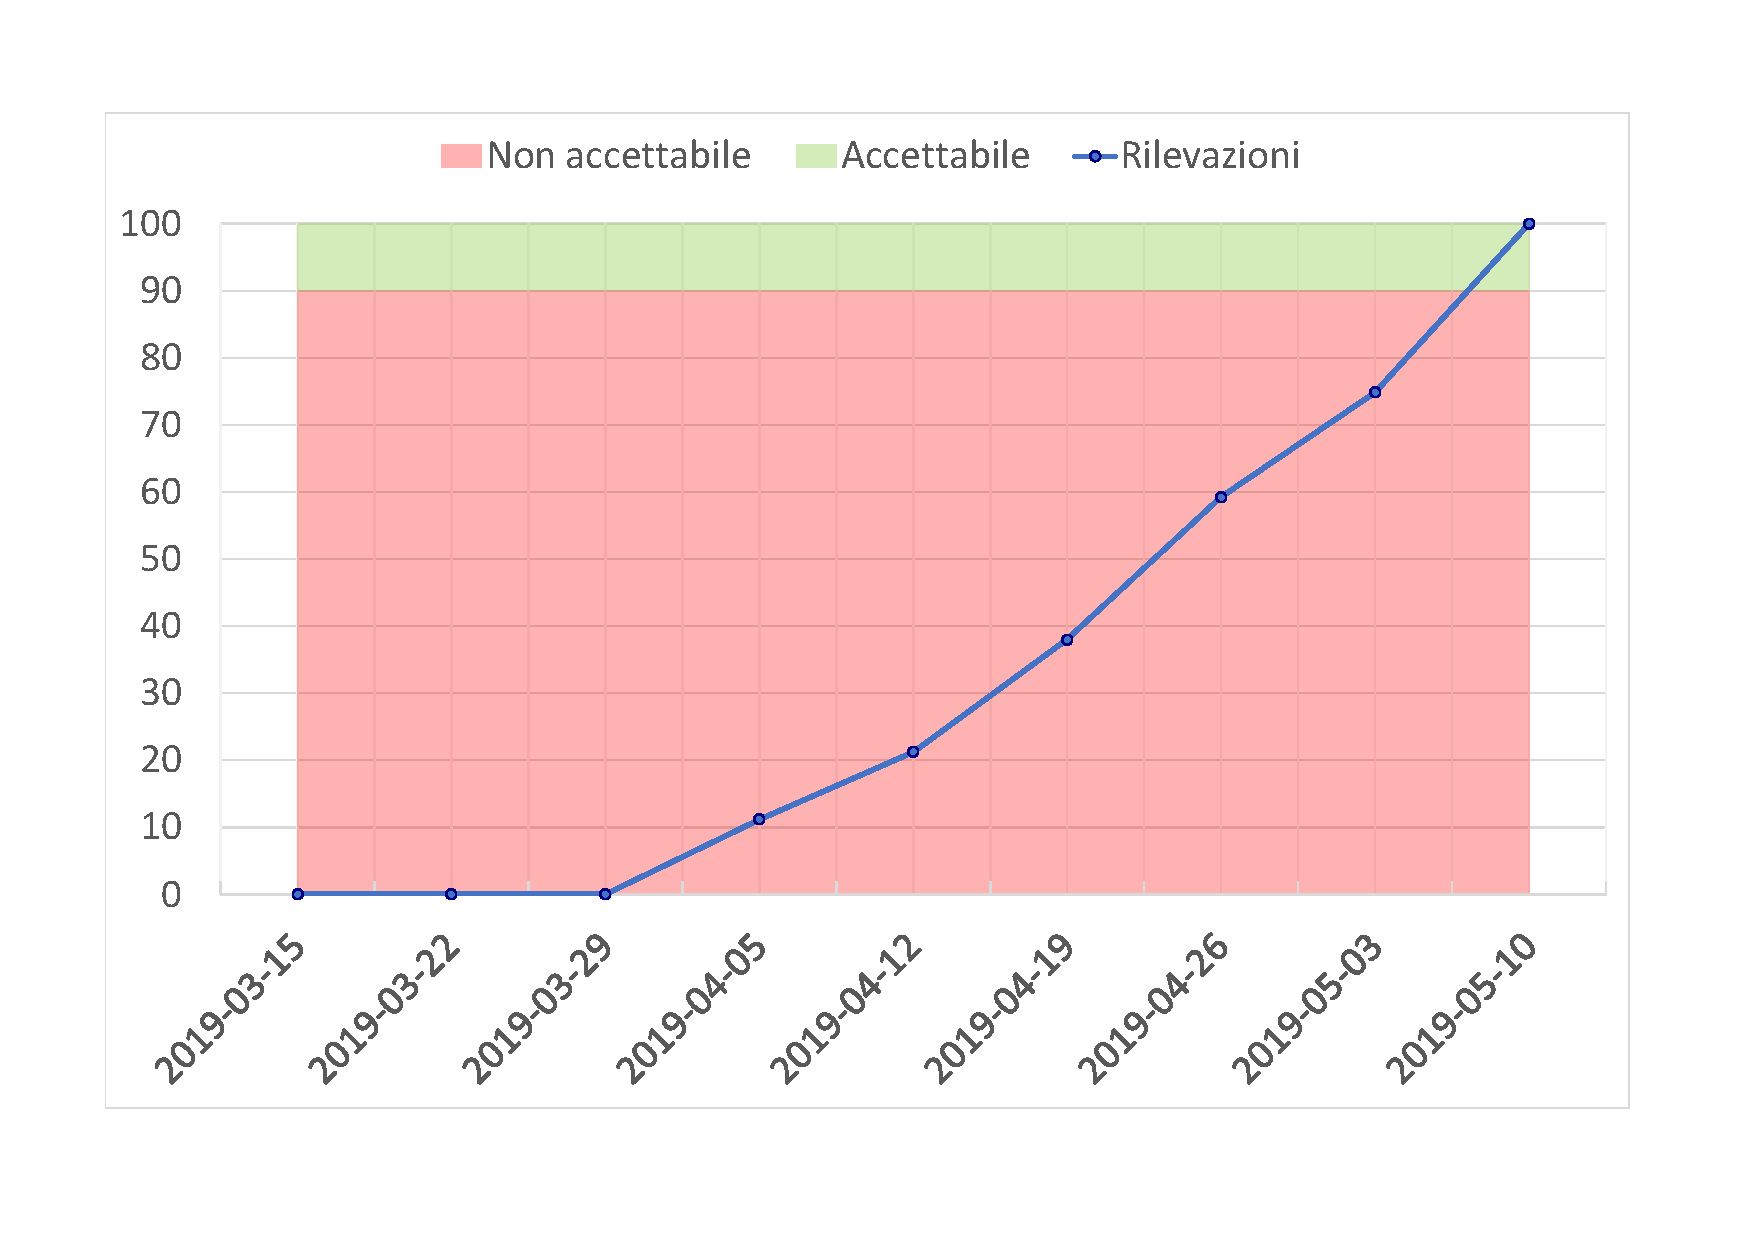
\includegraphics[scale=0.6]{images/resoconto/MPC6Chart.pdf}
	\caption{Serie storica test di unità implementati}	
\end{figure}

\subsubsection{Test di accettazione implementati - MPC7}
In questa fase non sono stati implementati test di accettazione.
Il gruppo si impegnerà all'implementazione degli stessi nella prossima fase.
\newpage
\subsection{Esito delle revisioni - RR}
Successivamente alla prima revisione formale, il gruppo ha apportato diverse modifiche ai documenti basandosi sulle osservazioni ricevute dai docenti. Le modifiche sono riassunte di seguito:
	\begin{itemize}
		\item \textbf{Norme di Progetto}: è stata aggiunta una sezione riportante le metriche di riferimento per processi e prodotti e la relativa normazione. 
		\item \textbf{Piano di Progetto}: le attività sono state ripianificate a partire dalla fase 2 ed è stato redatto un nuovo consuntivo.
		\item \textbf{Piano di Qualifica}: la struttura del documento è stata completamente rivista, i contenuti sono stati modificati secondo le indicazioni riportate nell'esito della prima revisione. Sono stati aggiunti diversi tipi di test e diverse appendici con argomenti vari; sono stati stabiliti degli obiettivi di qualità.
		\item \textbf{Analisi dei Requisiti}: sono stati aggiunti diversi nuovi casi d'uso, specializzando quelli già presenti e raddoppiandone il numero; sono stati modificati i diagrammi UML. \`E stata aggiunta una sezione introduttiva ed una descrizione degli attori implicati nel progetto. 
	\end{itemize}

\subsection{Esito delle revisioni - RP}	
Successivamente alla seconda revisione formale, il gruppo ha apportato diverse modifiche ai documenti basandosi sulle osservazioni ricevute dai docenti. Le modifiche sono riassunte di seguito:
	\begin{itemize}
		\item \textbf{Norme di Progetto}: sono state aggiunte diverse norme ed attività al processo di fornitura, revisionando contestualmente quelle già inserite. Sono state rimosse le soglie associate ad ogni metrica e la struttura del documento è stata in parte rivisitata.
		\item \textbf{Piano di Progetto}: le fasi 3 e 4 sono state ripianificate sulla base del periodo precedente; si è cercato di dare maggiore spessore all'incrementalità della logica di sviluppo adottata. 
		\item \textbf{Piano di Qualifica}: la struttura del documento è stata revisionata, sono stati redatti i test di unità e si è cercato di dare una struttura a cruscotto ai riscontri di verifica.
		\item \textbf{Analisi dei Requisiti}: i casi d'uso sono stati rivisti, aumentandone quanto possibile il livello di dettaglio; i codici dei casi d'uso e dei requisiti sono stati modificati e, di conseguenza, hanno subito modifiche anche i diagrammi UML.
	\end{itemize}

\subsection{Esito delle revisioni - RQ}	
Successivamente alla terza revisione formale, il gruppo ha apportato diverse modifiche ai documenti basandosi sulle osservazioni ricevute dai docenti. Le modifiche sono riassunte di seguito:
	\begin{itemize}
		\item \textbf{Norme di Progetto}: 
		\item \textbf{Piano di Progetto}: non sono state apportate modifiche rilevanti al documento
		\item \textbf{Piano di Qualifica}: sono stati aggiornati gli elenchi dei test applicati al sistema (di unità, integrazione, sistema e validazione) e la lista dei requisiti soddisfatti. 
		\item \textbf{Analisi dei Requisiti}: sono stati modificati i diagrammi UML per i casi UC-M1.3, UC-M3 e UC-I10.1, secondo le segnalazioni ricevute.
		\item \textbf{Manuale Utente}: sono stati riportati i requisiti hardware come segnalato ed il documento è stato completato.
		\item \textbf{Manuale Sviluppatore}: il documento è stato modificato secondo indicazioni ed i temi sono stati approfonditi in alcuni punti; il documento è stato poi completato.
	\end{itemize}
\newpage
\section{Copertura dei requisiti}
Viene riportata in seguito una tabella riassuntiva dei requisiti che non è da considerarsi definitiva, verrà infatti aggiornata in seguito ad ogni avanzamento significativo. \\
I requisiti sono indicati con il loro codice identificativo definito nel documento \textit{NormeDiProgetto\_v3.0.0} e la loro descrizione dettagliata è riportata nel documento \textit{AnalisiDeiRequisiti\_v3.0.0}.
\begin{longtable}{| p{2.5cm} | p{3cm} |}
	\rowcolor{LightBlue}
	\color{white}\bfseries Requisito & \color{white}\bfseries Stato \\
	ROF1 & Soddisfatto \\ \hline
	ROF2 & Soddisfatto \\ \hline
	ROF3 & Soddisfatto \\ \hline
	ROF4 & Soddisfatto \\ \hline
	ROF5 & Soddisfatto \\ \hline
	ROF6 & Soddisfatto \\ \hline
	ROF7 & Soddisfatto \\ \hline
	ROF8 & Soddisfatto \\ \hline
	ROF9 & Soddisfatto \\ \hline
	ROF10 & Soddisfatto \\ \hline
	ROF11 & Soddisfatto \\ \hline
	ROF12 & Soddisfatto \\ \hline
	ROF13 & Soddisfatto \\ \hline
	ROF14 & Soddisfatto \\ \hline
	ROF15 & Soddisfatto \\ \hline
	ROF16 & Soddisfatto \\ \hline
	ROF17 & Soddisfatto \\ \hline
	ROF18 & Soddisfatto \\ \hline
	ROF19 & Soddisfatto \\ \hline
	ROF20 & Soddisfatto \\ \hline
	ROF21 & Soddisfatto \\ \hline
	ROF22 & Soddisfatto \\ \hline
	ROF23 & Soddisfatto \\ \hline
	ROF24 & Soddisfatto \\ \hline
	ROF25 & Soddisfatto \\ \hline
	ROF26 & Soddisfatto \\ \hline
	ROF27 & Soddisfatto \\ \hline
	ROF28 & Soddisfatto \\ \hline
	ROF29 & Soddisfatto \\ \hline
	ROF30 & Soddisfatto \\ \hline
	ROF31 & Soddisfatto \\ \hline
	ROF32 & Soddisfatto \\ \hline
	ROF33 & Soddisfatto \\ \hline
	ROF34 & Soddisfatto \\ \hline
	ROF35 & Soddisfatto \\ \hline
	ROF36 & Soddisfatto \\ \hline
	ROF37 & Soddisfatto \\ \hline
	ROF38 & Soddisfatto \\ \hline
	ROF39 & Soddisfatto \\ \hline
	RDF1 & Soddisfatto \\ \hline
	RDF2 & Soddisfatto \\ \hline
	RDF3 & Soddisfatto \\ \hline
	RDF4 & Soddisfatto \\ \hline
	RDF5 & Soddisfatto \\ \hline
	RDF6 & Soddisfatto \\ \hline
	RDF7 & Soddisfatto \\ \hline
	RDF8 & Soddisfatto \\ \hline
	RDF9 & Soddisfatto \\ \hline
	RDF10 & Non soddisfatto \\ \hline
	RDF11 & Non soddisfatto \\ \hline
	RDF12 & Non soddisfatto \\ \hline
	RDF13 & Non soddisfatto \\ \hline
	RDF14 & Non soddisfatto \\ \hline
	RDF15 & Non soddisfatto \\ \hline
	RDF16 & Non soddisfatto \\ \hline
	RDF17 & Non soddisfatto \\ \hline
	RDF18 & Non soddisfatto \\ \hline
	RDF19 & Soddisfatto \\ \hline
	RDF20 & Non soddisfatto \\ \hline
	RDF21 & Non soddisfatto \\ \hline
	RDF22 & Soddisfatto\\ \hline
	RDF23 & Soddisfatto \\ \hline
	RDF24 & Soddisfatto \\ \hline
	RDF25 & Soddisfatto\\ \hline
	RDF26 & Non soddisfatto\\ \hline
	RDF27 & Non soddisfatto\\ \hline
	RDF28 & Soddisfatto \\ \hline
	RDF29 & Soddisfatto \\ \hline
	RDF30 & Soddisfatto \\ \hline
	RDF31 & Soddisfatto \\ \hline
	RDF32 & Soddisfatto \\ \hline
	RDF33 & Non soddisfatto\\ \hline
	RDF34 & Non soddisfatto \\ \hline
	RDF35 & Soddisfatto \\ \hline
	RDF36 & Non soddisfatto \\ \hline
	RDF37 & Non soddisfatto \\ \hline
	RDF38 & Soddisfatto \\ \hline
	RDF39 & Non soddisfatto \\ \hline
	RDF40 & Non soddisfatto \\ \hline
	RDF41 & Non soddisfatto \\ \hline
	RDF42 & Non soddisfatto \\ \hline
	RDF43 & Non soddisfatto \\ \hline
	RPF1 & Non soddisfatto \\ \hline
	RPF2 & Non soddisfatto \\ \hline
	RPF3 & Non soddisfatto \\ \hline
	RPF4 & Non soddisfatto \\ \hline
	RPF5 & Non soddisfatto \\ \hline
	RPF6 & Non soddisfatto \\ \hline
	RPF7 & Non soddisfatto \\ \hline
	RPF8 & Non soddisfatto \\ \hline
	RPF9 & Non soddisfatto \\ \hline
	RPF10 & Non soddisfatto \\ \hline
	RPF11 & Non soddisfatto \\ \hline
	RPF12 & Non soddisfatto \\ \hline
	RPF13 & Soddisfatto \\ \hline
	RPF14 & Non soddisfatto \\ \hline
	RPF15 & Soddisfatto \\ \hline
	RPF16 & Soddisfatto \\ \hline
	RPF17 & Non soddisfatto \\ \hline
	RPF18 & Non soddisfatto \\ \hline
	RPF19 & Non soddisfatto \\ \hline
	RPF20 & Soddisfatto \\ \hline
	RPF21 & Non soddisfatto \\ \hline
	RPF22 & Soddisfatto \\ \hline
	RPF23 & Non soddisfatto \\ \hline
	RPF24 & Non soddisfatto \\ \hline
	RPF25 & Non soddisfatto \\ \hline
	RPF26 & Non soddisfatto \\ \hline
	RPF27 & Soddisfatto \\ \hline
	RPF28 & Non soddisfatto \\ \hline
	RPF29 & Non soddisfatto \\ \hline
	RPF30 & Non soddisfatto \\ \hline
	ROV1 & Soddisfatto \\ \hline
	ROV2 & Soddisfatto \\ \hline
	ROV3 & Soddisfatto \\ \hline
	ROV4 & Soddisfatto \\ \hline
	RDV1 & Soddisfatto \\ \hline
	RPV1 & Non soddisfatto \\ \hline
	ROQ1 & Soddisfatto \\ \hline
	ROQ2 & Soddisfatto \\ \hline
	ROQ3 & Soddisfatto \\ \hline
	RDQ1 & Soddisfatto \\ \hline
	RDQ2 & Non soddisfatto \\ \hline
	RDQ3 & Soddisfatto \\ \hline
	RDQ4 & Non soddisfatto \\ \hline
	RDQ5 & Soddisfatto \\ \hline
	RPQ1 & Non soddisfatto \\ \hline
	\caption{Riassunto copertura requisiti}
\end{longtable}


	

	
\end{document}
